%%
%% This is file `sample-manuscript.tex',
%% generated with the docstrip utility.
%%
%% The original source files were:
%%
%% samples.dtx  (with options: `all,proceedings,bibtex,manuscript')
%% 
%% IMPORTANT NOTICE:
%% 
%% For the copyright see the source file.
%% 
%% Any modified versions of this file must be renamed
%% with new filenames distinct from sample-manuscript.tex.
%% 
%% For distribution of the original source see the terms
%% for copying and modification in the file samples.dtx.
%% 
%% This generated file may be distributed as long as the
%% original source files, as listed above, are part of the
%% same distribution. (The sources need not necessarily be
%% in the same archive or directory.)
%%
%%
%% Commands for TeXCount
%TC:macro \cite [option:text,text]
%TC:macro \citep [option:text,text]
%TC:macro \citet [option:text,text]
%TC:envir table 0 1
%TC:envir table* 0 1
%TC:envir tabular [ignore] word
%TC:envir displaymath 0 word
%TC:envir math 0 word
%TC:envir comment 0 0
%%
%%
%% The first command in your LaTeX source must be the \documentclass
%% command.
%%
%% For submission and review of your manuscript please change the
%% command to \documentclass[manuscript, screen, review]{acmart}.
%%
%% When submitting camera ready or to TAPS, please change the command
%% to \documentclass[sigconf]{acmart} or whichever template is required
%% for your publication.
%%
%%
\documentclass[manuscript,screen,review]{acmart}

\usepackage{caption}
\usepackage[utf8]{inputenc}
\usepackage[capitalize, noabbrev]{cleveref}
\usepackage{xcolor}
\usepackage{enumitem}

\usepackage{pgfplots}
\usepackage{listings}

\lstdefinestyle{prompt}{
  basicstyle=\small,
  breaklines=true,
  breakindent=0pt,
  frame=single,
  escapeinside={\%*}{*)},  % if you want to add LaTeX within your code
}

\lstset{
  basicstyle=\small, % or \footnotesize, \scriptsize, etc.
  % other settings
}

\newcommand{\highlight}[1]{\textcolor{blue}{\textbf{#1}}}

% commands for the findings box
\newcommand{\findingsbox}[1]{%
  \vspace{8pt}%
  \noindent%
  \setlength{\fboxsep}{-0.25pt}% 
  \setlength{\fboxrule}{0pt}%
  \fbox{%
  \setlength{\fboxrule}{0.25pt}%
    \fcolorbox{gray!90}{gray!10}{%
      \parbox{\dimexpr\columnwidth-2\fboxsep-2\fboxrule}{%
        {\color{gray!90}\vrule width 6pt}%
        \hspace{10pt}%
        \parbox{\dimexpr\columnwidth-4\fboxsep-4\fboxrule-29pt}{%
          \color{black}% 
          \vspace{8pt}% 
          #1%
          \vspace{8pt}%
        }%
      }%
    }%
  }%
}   


%%
%% \BibTeX command to typeset BibTeX logo in the docs
\AtBeginDocument{%
  \providecommand\BibTeX{{%
    Bib\TeX}}}

%% Rights management information.  This information is sent to you
%% when you complete the rights form.  These commands have SAMPLE
%% values in them; it is your responsibility as an author to replace
%% the commands and values with those provided to you when you
%% complete the rights form.
\setcopyright{acmlicensed}
\copyrightyear{2024}
\acmYear{2024}
\acmDOI{XXXXXXX.XXXXXXX}

%% These commands are for a PROCEEDINGS abstract or paper.
\acmConference[Koli Calling '24]{24th Koli Calling International Conference on Computing Education Research}{November 14--17,
  2024}{Koli, Finland}
%%
%%  Uncomment \acmBooktitle if the title of the proceedings is different
%%  from ``Proceedings of ...''!
%%
%%\acmBooktitle{Woodstock '18: ACM Symposium on Neural Gaze Detection,
%%  June 03--05, 2018, Woodstock, NY}
% \acmISBN{978-1-4503-XXXX-X/18/06}


%%
%% Submission ID.
%% Use this when submitting an article to a sponsored event. You'll
%% receive a unique submission ID from the organizers
%% of the event, and this ID should be used as the parameter to this command.
%%\acmSubmissionID{123-A56-BU3}

%%
%% For managing citations, it is recommended to use bibliography
%% files in BibTeX format.
%%
%% You can then either use BibTeX with the ACM-Reference-Format style,
%% or BibLaTeX with the acmnumeric or acmauthoryear sytles, that include
%% support for advanced citation of software artefact from the
%% biblatex-software package, also separately available on CTAN.
%%
%% Look at the sample-*-biblatex.tex files for templates showcasing
%% the biblatex styles.
%%

%%
%% The majority of ACM publications use numbered citations and
%% references.  The command \citestyle{authoryear} switches to the
%% "author year" style.
%%
%% If you are preparing content for an event
%% sponsored by ACM SIGGRAPH, you must use the "author year" style of
%% citations and references.
%% Uncommenting
%% the next command will enable that style.
%%\citestyle{acmauthoryear}


%%
%% end of the preamble, start of the body of the document source.
\begin{document}

%%
%% The "title" command has an optional parameter,
%% allowing the author to define a "short title" to be used in page headers.
% \title{Automated Feedback Loops: Enhancing Student Motivation and Performance in Programming Courses}
\title{Direct Automated Feedback Delivery for Student Submissions based on LLMs}

%%
%% The "author" command and its associated commands are used to define
%% the authors and their affiliations.
%% Of note is the shared affiliation of the first two authors, and the
%% "authornote" and "authornotemark" commands
%% used to denote shared contribution to the research.


\author{Maximilian Sölch}
\email{maximilian.soelch@tum.de}
\orcid{0009-0004-1509-7842} 
\affiliation{%
	\institution{Technical University of Munich}
	\city{Munich}
	\country{Germany}
}

\author{Felix T.J. Dietrich}
\email{felixtj.dietrich@tum.de}
\orcid{0009-0007-5826-2061} 
\affiliation{%
	\institution{Technical University of Munich}
	\city{Munich}
	\country{Germany}
}

\author{Stephan Krusche}
\email{krusche@tum.de}
\orcid{0000-0002-4552-644X}
\affiliation{%
	\institution{Technical University of Munich}
	\city{Munich}
	\country{Germany}
}

%%
%% By default, the full list of authors will be used in the page
%% headers. Often, this list is too long, and will overlap
%% other information printed in the page headers. This command allows
%% the author to define a more concise list
%% of authors' names for this purpose.
\renewcommand{\shortauthors}{Sölch et al.}

%%
%% The abstract is a short summary of the work to be presented in the
%% article.
\begin{abstract}

Timely and individualized feedback is crucial for students' learning progress and motivation.
However, providing such feedback is a major challenge in education, especially as the number of students has steadily increased in recent years.
This growth has made it difficult for teachers to provide individualized feedback to each student, resulting in a time-consuming, repetitive and often manual task that contributes to a high workload.

This paper presents Direct Automated Feedback (DAFeeD), a large language model (LLM)-based approach for automated formative feedback on student submissions in various exercise domains.
The defined feedback process enables interactive learning by allowing students to submit their solutions multiple times and request feedback repeatedly before the submission deadline.
By incorporating task-specific information into the prompt, DAFeeD provides iterative customized feedback, facilitating continuous student improvement.

To empirically evaluate the feedback process, we implemented it in an open-source reference implementation that is integrated into the LMS learning platform.
We conducted a controlled study in which students used the feedback process in a programming task in a supervised environment and completed a survey.
%TODO: nächsten Zwei sätze sind zu schwach, mehr auf Vorteile eingehen
The results show that students perceive the feedback process as relevant and beneficial to their learning.
Students indicated that they feel more comfortable and willing to request automated feedback than they would with human tutors because it is more convenient and immediate.
This shows that DAFeeD has the potential to significantly improve the feedback process in educational institutions and increase students' learning efficiency and performance.

\end{abstract}

%%
%% The code below is generated by the tool at http://dl.acm.org/ccs.cfm.
%% Please copy and paste the code instead of the example below.
%%
\begin{CCSXML}
  <ccs2012>
     <concept>
         <concept_id>10003456.10003457.10003527.10003540</concept_id>
         <concept_desc>Social and professional topics~Student assessment</concept_desc>
         <concept_significance>500</concept_significance>
         </concept>
     <concept>
         <concept_id>10010405.10010489</concept_id>
         <concept_desc>Applied computing~Education</concept_desc>
         <concept_significance>500</concept_significance>
         </concept>
   </ccs2012>
\end{CCSXML}
  
\ccsdesc[500]{Social and professional topics~Student assessment}
\ccsdesc[500]{Applied computing~Education}

%%
%% Keywords. The author(s) should pick words that accurately describe
%% the work being presented. Separate the keywords with commas.
\keywords{Software Engineering, Education, Formative Feedback, Interactive Learning}

% \received{20 February 2007}
% \received[revised]{12 March 2009} 
% \received[accepted]{5 June 2009}

%%
%% This command processes the author and affiliation and title
%% information and builds the first part of the formatted document.
\maketitle

\section{Introduction} % 1 page

% problem
% time consuming, not scalable, not always available
% hinders learning progress and motivation

% todo: reference for this! \cite{jonsson:2013:FacilitatingProductiveUse} \cite{shute:2008:FocusFormativeFeedback}
In the current educational landscape, providing timely and effective feedback to students remains a significant challenge.
Traditionally, students must wait for course tutors or professors to review their submissions and provide feedback.
This process can be time-consuming, often requiring students to arrange meetings and wait for available time slots, which are not always convenient or immediate.
Similar it is time-consuming and tedious for professors and tutors to provide asynchronous feedback via email or other communication channels \cite{henderson:2019:ChallengesFeedbackHigher}.
The inherent delays and scheduling difficulties make this approach not scalable, especially in courses with a large number of students.

Additionally, providing individualized feedback and enabling students to enhance their knowledge through formative assessments are crucial components of effective learning \cite{irons:2007:EnhancingLearningFormative,higgins:2002:ConscientiousConsumerReconsidering}.
However, the limited availability of tutors and professors means that not all students receive the individualized attention they need to improve their understanding and skills.
This situation underscores the necessity for a more efficient and scalable feedback system that can provide continuous support and formative feedback to students without the constraints of traditional methods \cite{sondergaard:2004:EffectiveFeedbackSmall}.
Such a feedback system enables interactive learning for students, increasing their engagement in the course resulting in better final grades \cite{krusche:2017:InteractiveLearningIncreasing}.

% Objectives
In this paper, we present DAFeeD, an approach for generating automated feedback on student submissions using large language models (LLMs), to address these challenges.
The approach is independent of the exercise type and can be applied to various domains, such as programming, text, or modeling exercises.
We implemented the approach in an open-source reference implementation called Athena, connected to the learning platform Artemis \cite{krusche:2018:ArTEMiSAutomaticAssessmentf} through which students submit their solutions and receive feedback.
To validate the effectiveness and efficiency of the approach, we tested it in a controlled environment. 
% We collected quantitative and qualitative data to evaluate students' perceptions of the approach and the overall performance of the reference implementation.
% The results show that students perceive the feedback process as relevant and beneficial to their learning, indicating that the approach has the potential to significantly improve the feedback process in educational institutions and increase students' learning efficiency and performance.

With this paper, we want to answer the following research questions about direct automated feedback delivery:

\begin{enumerate}[label=\textbf{RQ\arabic*},ref=RQ\arabic*]
  \item \label{RQ1} How does the availability of direct automated feedback affect student engagement and motivation? 
  \item \label{RQ2} Do students feel more comfortable requesting automatic feedback than asking a human tutor or the course professor?
  \item \label{RQ3} How do students perceive the effectiveness of direct automated feedback?
  \item \label{RQ4} How do students perceive the usability and helpfulness of DAFeeD?
\end{enumerate}


%Outline
The subsequent sections of this paper are organized to provide a comprehensive understanding of the research. 
\cref{sec:related-work} provides an overview of related work. 
\cref{sec:approach:DAFeeD} details the concept and methodology of Direct Automated Feedback Delivery (DAFeeD).
\cref{sec:reference-implementation} describes the reference implementation of DAFeeD, called Athena, including a general overview, details on the used prompts, and the system architecture. 
\cref{sec:evaluation} presents the evaluation results, including the research questions, study design, and findings. 
Finally, \cref{sec:conclusion} concludes with a summary of findings and discusses future research directions to enhance automated feedback systems.

%\newpage
\section{Related Work} % 2 page
\label{sec:related-work}

% A Systematic Review of the Effects of Automatic Scoring and Automatic Feedback in Educational Settings
% \citet{hahn:2021:SystematicReviewEffects}
Automated feedback systems have gained significant attention in educational research due to their potential to scale online education and reduce the time between submission and feedback. \citet{hahn:2021:SystematicReviewEffects} conducted a systematic review on the effects of automatic scoring and feedback tools, emphasizing their crucial role in enhancing scalability, reducing bias, and increasing student engagement. Their insights highlight the broader implications of automated feedback systems in education, which is highly relevant to our study.


% A Systematic Literature Review of Automated Feedback Generation for Programming Exercises
% \citet{keuning:2018:SystematicLiteratureReview} 
%
% -> Extension for potential of LLMs:
% Exploring the Potential of Large Language Models to Generate Formative Programming Feedback
% \citet{kiesler:2023:ExploringPotentialLarge} 
In the domain of programming education, \citet{keuning:2018:SystematicLiteratureReview} reviewed 101 tools for automated feedback on programming exercises. They noted that most tools focus on error identification rather than providing actionable guidance or adapting to specific instructional needs. Extending this work, \citet{kiesler:2023:ExploringPotentialLarge} explored the effectiveness of large language models (LLMs) like ChatGPT in generating formative programming feedback, finding that while LLMs can produce useful feedback, they often include misleading information for novices. This emphasizes the need for careful design and evaluation of LLM-based feedback systems to ensure reliability and accuracy.


% How Novices Use LLM-based Code Generators to Solve CS1 Coding Tasks in a Self-Paced Learning Environment
% \citet{kazemitabaar:2024:HowNovicesUse}
%
% To trust or to think: Cognitive forcing functions can reduce overreliance on AI in AI-assisted decision-making.
% \citet{bucinca:2021:TrustThinkCognitive}
%
% Programming Is Hard - Or at Least It Used to Be: Educational Opportunities and Challenges of AI Code Generation
% \citet{becker:2023:ProgrammingHardLeast}
\citet{kazemitabaar:2024:HowNovicesUse} examined how novice programmers interact with LLM-based code generators in self-paced learning environments. They identified distinct usage patterns and their impact on learning outcomes, revealing that a ``Hybrid'' approach — combining manual coding with LLM assistance — was most beneficial for learners. This aligns with findings by \citet{bucinca:2021:TrustThinkCognitive}, who highlighted the dangers of over-reliance on AI and proposed cognitive forcing functions to encourage deeper engagement with AI outputs. Similarly, \citet{becker:2023:ProgrammingHardLeast} discussed both the opportunities and challenges of AI-driven code generation tools, emphasizing the need for educators to guide students in leveraging these technologies effectively without becoming dependent on them. These findings highlight the importance of balancing AI assistance with traditional learning methods, which is a key consideration in our DAFeeD system.


% Focus on Formative Feedback
% \citet{shute:2008:FocusFormativeFeedback} 
%
% What makes for effective feedback: staff and student perspectives
% \citet{dawson:2019:WhatMakesEffective}
The importance of timely and specific feedback is well-documented. \citet{shute:2008:FocusFormativeFeedback} provided a comprehensive review of formative feedback, highlighting its necessity for being nonevaluative, supportive, timely, and specific. \citet{dawson:2019:WhatMakesEffective} further explored perceptions of effective feedback, revealing that while educators focus on design aspects such as timing and modalities, students prioritize the quality and usability of feedback comments. This underscores the need for automated feedback systems to deliver not only timely but also detailed, specific, and personalized comments.


% Adaptive Immediate Feedback Can Improve Novice Programming Engagement and Intention to Persist in Computer Science
% \citet{marwan:2020:AdaptiveImmediateFeedback}
%
% A Comparison of Immediate and Scheduled Feedback in Introductory Programming Projects
% \citet{leinonen:2022:ComparisonImmediateScheduled}
Adaptive and immediate feedback mechanisms have been shown to significantly enhance student learning outcomes. \citet{marwan:2020:AdaptiveImmediateFeedback} demonstrated that adaptive and immediate feedback can improve student performance and motivation. Similarly, \citet{leinonen:2022:ComparisonImmediateScheduled} compared immediate and scheduled feedback, concluding that immediate feedback is more effective in promoting student engagement and timely corrections. These studies collectively stress the potential of automated feedback systems in providing timely, adaptive, and engaging feedback, crucial for continuous improvement and learning efficiency.


% Feedback-Generation for Programming Exercises With GPT-4:
% Imen Azaiz, Natalie Kiesler, and Sven Strickroth. 2024. Feedback-Generation for Programming Exercises With GPT-4. arXiv:2403.04449 [cs]
% Accepted at ITiCSE '24, first author is from LMU
The work by \citet{azaiz:2024:FeedbackGenerationProgrammingExercises} highlights the limitations of LLMs, advising against using GPT-4 Turbo for automatic feedback generation in programming education due to inconsistencies. In contrast, our research with DAFeeD evaluates an integrated direct automatic feedback delivery process within a Learning Management System (LMS), demonstrating its potential immediate benefits for students, especially when feedback is critically evaluated. We believe that increasingly powerful LLMs and advanced prompting strategies will enhance feedback quality over time, with appropriate guardrails to prevent revealing solutions.


% CodeHelp: Using Large Language Models with Guardrails for Scalable Support in Programming Classes
% \citet{liffiton:2024:CodeHelpUsingLarge}
The study by \citet{liffiton:2024:CodeHelpUsingLarge} introduces CodeHelp, an LLM-powered tool that provides real-time assistance to programming students. In a first-year computer science course with 52 students, CodeHelp collected data over 12 weeks, revealing that students valued its availability, immediacy, and support for error resolution and independent learning. CodeHelp requires students to manually enter code, error messages, and issue descriptions. In contrast, DAFeeD integrates into the LMS, automatically providing context and feedback on code repository changes without requiring student input. This seamless integration aims to increase student engagement and motivation by offering timely, individualized feedback automatically, and to improve perceptions of feedback effectiveness, usability, and helpfulness.


% Using GPT-4 to Provide Tiered, Formative Code Feedback
% \citet{nguyen:2024:UsingGPT4Providea}
Similarly, \citet{nguyen:2024:UsingGPT4Providea} demonstrate the feasibility of using GPT-4 for tiered, formative feedback on programming exercises in introductory courses, providing insights on conceptual understanding, syntax, and time complexity. Our DAFeeD approach is evaluated using a similar LLM, GPT-4 Turbo, and likewise focuses on providing formative feedback in introductory courses. However, while \citeauthor{nguyen:2024:UsingGPT4Providea} provide feedback on isolated code snippets using few-shot learning, DAFeeD delivers iterative feedback on entire repositories with multiple files using detailed prompts and context collection. Additionally, DAFeeD is integrated directly into an LMS, supporting multiple exercise domains, which allows students to iteratively improve their submissions before the deadline, aiming to enhance learning outcomes and engagement through interactive learning.


% AI Teaches the Art of Elegant Coding: Timely, Fair, and Helpful Style Feedback in a Global Course
% \citet{woodrow:2024:AITeachesArta}
\citet{woodrow:2024:AITeachesArt} explore the deployment and effectiveness of a real-time style feedback tool using LLMs, specifically GPT 3.5 Turbo, in a large-scale online CS1 course. Their findings indicate significant improvements in student engagement and coding style when feedback is immediate and integrated within the learning platform. \citeauthor{woodrow:2024:AITeachesArt} conducted a randomized control trial with over 8,000 students, demonstrating that real-time feedback was five times more likely to be viewed and incorporated by students compared to delayed feedback. This supports our approach with DAFeeD, emphasizing the importance of immediate, individualized feedback in enhancing student learning outcomes.

A broader perspective on the capabilities and challenges of LLMs is provided by \citet{wei:2022:EmergentAbilitiesLarge}, who discussed the emergent abilities of large language models that are not present in smaller models, highlighting the need for ongoing research to harness these capabilities effectively. \citet{huang:2023:SurveyHallucinationLargeb} addressed the issue of hallucinations in LLMs, offering an in-depth overview of detection methods and mitigation strategies crucial for developing reliable feedback systems. \citet{amatriain:2024:PromptDesignEngineering} detailed core concepts and advanced techniques in prompt engineering, such as Chain-of-Thought and Reflection, which can enhance the quality and relevance of automated feedback. Additionally, \citet{liu:2024:JailbreakingChatGPTPrompt} highlighted the importance of robust prompt design to prevent misuse, investigating vulnerabilities of LLMs to jailbreak prompts. \citet{zhao:2023:SurveyLargeLanguage} reviewed the evolution and recent advances of large language models, focusing on pre-training, adaptation tuning, utilization, and capacity evaluation, and highlighting the progress and ongoing challenges in the field. Lastly, \citet{yang:2024:HarnessingPowerLLMs} provided a comprehensive guide for practitioners working with LLMs, discussing the influence of pre-training data and challenges associated with different natural language processing tasks, offering insights for developing and deploying LLM-based feedback systems.

In summary, the related work collectively highlights the evolving landscape of automated feedback systems and the significant potential of LLMs to enhance educational outcomes through immediate, specific, and actionable feedback. Our primary contribution with DAFeeD lies in its seamless integration within the LMS, supporting a variety of exercise types. By LLMs, DAFeeD provides individualized formative feedback automatically, with a focus on the feedback delivery process rather than the current quality. We are confident that feedback quality will improve through more advanced prompting methods as LLM technology evolves. This approach enables students to iteratively improve their solutions and learn continuously without direct intervention from tutors or professors. Ultimately, DAFeeD aims to enhance student engagement, learning efficiency, and performance through timely, relevant, and personalized feedback, aligning with and advancing the findings of the reviewed studies.

% ================

% A review of automated feedback systems for learners: Classification framework, challenges, and opportunities.
% \citet{deeva:2021:ReviewAutomatedFeedback}
% Felix: Won't include (for now)

% Grounded copilot: How programmers interact with code-generating models.
% \citet{barke:2023:GroundedCopilotHow}
% Felix: Won't include (for now)

% Studying the effect of AI Code Generators on Supporting Novice Learners in Introductory Programming
% \citet{kazemitabaar:2023:StudyingEffectAIa
% Felix: Won't include (for now)

% Exploring the Responses of Large Language Models to Beginner Programmers’ Help Requests
% \citet{hellas:2023:ExploringResponsesLargea}
% Felix: Won't include (for now)

% Investigating the Potential of GPT-3 in Providing Feedback for Programming Assessments
% \citet{balse:2023:InvestigatingPotentialGPT3}
% Felix: Won't include (for now)

% Using Large Language Models to Enhance Programming Error Messages
% \citet{leinonen:2023:UsingLargeLanguagea}
% Felix: Won't include (for now)

% Next-Step Hint Generation for Introductory Programming Using Large Language Models
% \citet{roest:2024:NextStepHintGeneration}
% Felix: Won't include (for now)

% Design principles for generating and presenting automated formative feedback on code quality using software metrics
% \citet{vandenaker:2024:DesignPrinciplesGeneratingb}
% Felix: Won't include (for now)

% PyDex: Repairing Bugs in Introductory Python Assignments using LLMs
% \citet{zhang:2024:PyDexRepairingBugs}
% Felix: Won't include (for now)

% =====================

%\newpage
\section{Approach: Direct Automated Feedback Delivery (DAFeeD)} % 1 page
\label{sec:approach:DAFeeD}

DAFeeD employs large language models to deliver automated feedback on student submissions, designed to complement traditional teaching methods and provide additional support.
Figure \ref{fig:DAFeeD-workflow} illustrates the continuous feedback workflow that DAFeeD facilitates, enabling students to receive feedback at any time, thereby eliminating the need to wait for responses from human tutors or course professors.

\begin{figure}[htbp]
  \centering
  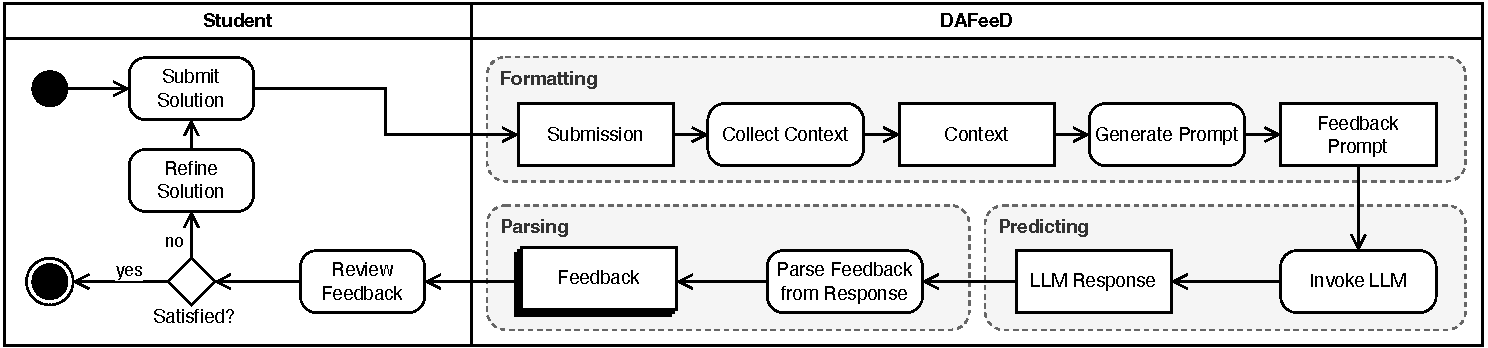
\includegraphics[width=\linewidth]{figures/DAFeeD-ActivityDiagram_alternative.pdf}
  \caption{UML activity diagram of the Direct Automated Feedback Delivery (DAFeeD) workflow for student submissions.}
  \label{fig:DAFeeD-workflow}
\end{figure}

The feedback process is designed to be exercise-independent, meaning that it can be applied to various exercise types, such as programming, text, or modeling exercises.
%todo: cite formative feedback
DAFeeD can provide formative feedback to the students, including feedback on issues or improvements, as well as positive feedback when the student completes the task correctly.
Once the student submits their solution, DAFeeD initiates a three-stage process to generate natural language feedback.

%todo: add learner profile (find reference) to generate individualized, personal feedback tailored to the student's learning progress and needs.
The first stage, called \textit{Formatting}, takes the student's submission and extracts the submission content, the problem statement, including learning objectives, and any possible grading instructions the instructor defines.
All of this gathered information represents the context.
During the prompt generation step, a predefined prompt template is filled with the prompt input data, resulting in the feedback prompt.
Depending on the exercise, adaptions need to be made to the prompt template to ensure that the feedback output of the LLM is tailored to the specific exercise type.
For programming exercises, the generated feedback needs to have metadata information about the file and line number of the code snippet to which the feedback refers.
For text exercises, the feedback needs to have metadata about the sentence or word range the feedback refers to.

In the second stage, called \textit{Predicting}, DAFeeD sends the feedback prompt to a large language model (LLM) and invokes it with the prompt. 
As a result, the LLM generates a response to that prompt including detailed feedback items for the student.

The final stage, \textit{Parsing}, takes the LLM response, which comes in the JSON format, and parses feedback items from it. 
In addition to the feedback text, the feedback object also contains reference information indicating the part of the submission it pertains to.
For programming exercises, this includes the file name and line number of the relevant code snippet to which the feedback refers.
For text exercises, the reference information includes only the sentence or word range the feedback refers to.

All of the feedback is then returned to the student for review.
If the student is satisfied with the feedback, the process concludes. 
Otherwise, the student can refine and resubmit their solution, initiating the DAFeeD process anew.

This iterative process is designed to motivate students to continuously learn and experiment with their solutions, resulting in improved performance.


\section{Reference Implementation: Athena} % 2 pages
\label{sec:reference-implementation}

We incorporated DAFeeD into a reference implementation named Athena, which is seamlessly integrated with the learning platform Artemis. 
Through Artemis, students can submit their solution and review the feedback.

When submitting their solutions on Artemis, students have the option to request direct automated feedback by clicking a newly added button.
This feedback request is then sent to Athena, provided the student has not reached their feedback request limit for the exercise.
Course instructors can customize the number of allowed feedback requests per exercise according to their preference.
A status visualization informs students about their feedback request state.
Once Athena generates the feedback and sends it back to Artemis, the student can review it in a modal window on Artemis, as depicted in Figure \ref{fig:Artemis-feedback-visualization}.


\begin{figure}[htbp]
  \centering
  \includegraphics[width=0.75\linewidth]{figures/athena-feedback-new_light_clarity-upscaler_annonymized.png}
  \caption{Visualization of the feedback interface in the LMS as seen by students.}
  \label{fig:Artemis-feedback-visualization}
\end{figure}


\subsection{Feedback Generation}

The prompt design is crucial for guiding the large language model (LLM) in generating effective and contextually relevant feedback. For this study, we utilized OpenAI's GPT-4 Turbo with a temperature setting of 0 to ensure deterministic and consistent feedback generation, reducing randomness and the potential for hallucinations. However, the system is configurable, allowing the use of other models and settings. In Figure \ref{fig:prompt-programming-exercise-generation}, we provide an example of a prompt used for generating feedback for programming exercises. 
This prompt incorporates specific instructions to ensure that the feedback is individualized to the student's submission while not revealing the solution.

The feedback generation process for programming exercises begins by identifying the differences between the student's submission repository and the provided template repository, the starting point. 
These differences are identified using a git diff, which highlights lines removed and added by the student. 
If the problem statement is too lengthy or complex, a separate LLM invocation is used to split the problem statement into relevant parts for each file. 
This ensures that the feedback is targeted and relevant to the specific context of the file being reviewed. 
Additionally, a summary of the student's solution across all files is generated using another LLM invocation. 
This summary provides a comprehensive overview of the submission, which is included in the prompt to offer context for the feedback.

In the provided prompt, several key components guide the LLM in creating useful feedback. The \textit{Problem Statement} section contextualizes the student's task and helps the LLM understand the exercise's objectives.
The \textit{Task Instructions} direct the LLM to provide non-graded, formative feedback focusing on educational aspects without offering direct solutions.
\textit{Style Guidelines} ensure the feedback is constructive, specific, balanced, clear, concise, actionable, educational, and contextual.
The \textit{File Path and Content} provide the specific file under review along with its content, aiding the LLM in pinpointing specific lines of code for feedback.
Additionally, \textit{Summary and Diffs} between the template and submission offer additional context, helping the LLM understand the student's changes and their overall approach.

The structure and content of this prompt are designed to emulate a human tutor's approach, ensuring that the feedback is both relevant and supportive of the student's learning process.
By providing such detailed instructions and contextual information, the LLM can generate feedback that is both meaningful and actionable for students.

% Prompt for generating feedback suggestions of programming exercises
\begin{figure}[!htbp]
  \begin{lstlisting}[style=prompt]
You are an AI tutor for programming exercises at a prestigious university.

# Problem statement
%*\highlight{\{problem\_statement\}}*)

# Task
Provide non-graded formative feedback on a student's programming submission as a human tutor would. The tutor is not familiar with the solution, so the feedback should focus solely on aspects from which the student can learn. This feedback must highlight incorrectly applied principles or inconsistencies without offering specific solutions or error corrections. Allow some flexibility for students to deviate from the problem statement, provided they complete all tasks. Ensure the feedback is balanced and comprehensive.

# Style
1. Constructive, 2. Specific, 3. Balanced, 4. Clear and Concise, 5. Actionable, 6. Educational, 7. Contextual

Feedback that contradicts the problem statement is strictly prohibited. Avoid mentioning aspects not explicitly covered in the template to submission diff, such as the exercise package name, as these are beyond the student's control.

In git diff, lines marked with '-' were removed and with '+' were added by the student.

The student will be reading your response, so use "you" instead of "them".

Path: %*\highlight{\{submission\_file\_path\}}*)

File (with line numbers <number>: <line>):
%*\highlight{\{submission\_file\_content\}}*)

Summary of other files in the solution:
%*\highlight{\{summary\}}*)

The template to submission diff (only as reference):
%*\highlight{\{template\_to\_submission\_diff\}}*)
  \end{lstlisting}
  \caption{Prompt template for generating feedback for programming exercises.}
  \label{fig:prompt-programming-exercise-generation}
\end{figure}

\subsection{Architecture}

Athena is deployed in production alongside the learning platform Artemis, which serves up to more than 2000 students per course.
Consequently, the reference implementation must satisfy additional non-functional requirements such as performance, scalability, maintainability, and usability.
To meet these requirements and to support feedback generation for multiple exercise types while allowing for future extensibility, we adopted a modular architecture, as illustrated in Figure \ref{fig:Athena-architecture}.

% Felix:
% - Components could be vertically slightly smaller 
\begin{figure}[htbp]
  \centering
  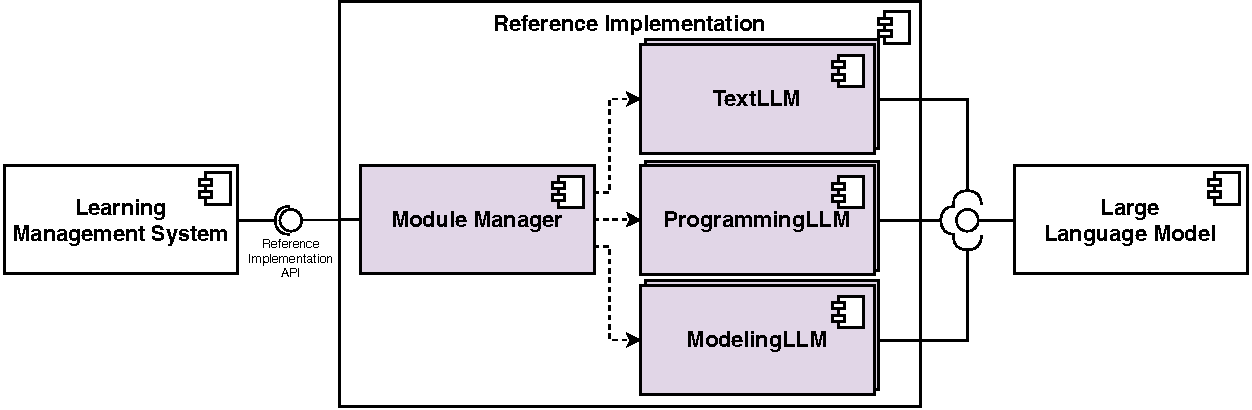
\includegraphics[width=0.8\linewidth]{figures/Athena-Architecture.pdf}
  \caption{UML component diagram of the top-level architecture of the reference implementation.}
  \label{fig:Athena-architecture}
\end{figure}

The \textit{Module Manager} handles all incoming requests, verifies authorization, and forwards them to the appropriate modules.
The \textit{ProgrammingLLM} module manages programming exercises and executes the three-stage DAFeeD process, which includes formatting, predicting, and parsing. 
Similarly, the \textit{TextLLM} module is optimized for text exercises and follows the same process.

Athena's system design is independent of any specific learning management system (LMS) as it provides a REST API, documented using the OpenAPI standard\footnote{\url{https://www.openapis.org}}.
This independence allows Athena to be integrated with various LMS platforms, such as Moodle\footnote{\url{https://moodle.org}}.

Athena currently connects to OpenAI models hosted in a private Azure cloud to ensure that student data is not used for training models, maintaining privacy.
Additionally, the system can be configured to use open-source models like Llama\footnote{\url{https://llama.meta.com}} or Mistral\footnote{\url{https://mistral.ai}}, either self-hosted or cloud-based.

To meet performance and scalability requirements, Athena and its modules are deployed within a Kubernetes cluster\footnote{\url{https://kubernetes.io}}.
Kubernetes, in conjunction with Athena's modular architecture, allows the system to scale each module independently.
For example, additional instances of the programming module can be instantiated when a new programming exercise is released.
Furthermore, Kubernetes provides out-of-the-box load balancing and self-healing capabilities, ensuring that if a module crashes, it is automatically restarted.


\section{Evaluation} % 5 pages
\label{sec:evaluation}

In this section, we outline the methodology employed to validate the effectiveness of the proposed DAFeeD approach including the reference implementation Athena.
The conducted evaluation represents the treatment validation stage of the design science methodology proposed by Wieringa \cite{wieringa:2014:DesignScienceMethodologya}.
In this stage, the proposed solution — DAFeeD — is evaluated in a controlled environment, and the collected data is utilized for the refinement and improvement of the solution.

We begin by describing the study design and the results.
Subsequently, we outline the limitations of the evaluation and discuss the implications of the findings.


% research questions moved to the introduction
% \subsection{Research Questions}

% With this study, we want to answer the following research questions about direct automated feedback delivery:

% \begin{enumerate}[label=\textbf{RQ\arabic*},ref=RQ\arabic*]
%   \item \label{RQ1} How does the availability of direct automated feedback affect student engagement and motivation? 
%   \item \label{RQ2} Do students feel more comfortable requesting automatic feedback than asking a human tutor or the course professor?
%   \item \label{RQ3} How do students perceive the effectiveness of direct automated feedback?
%   \item \label{RQ4} How do students perceive the usability and helpfulness of DAFeeD?
% \end{enumerate}

% \ref{RQ1} examines the influence of direct automated feedback on students' overall engagement with the course material and their motivation to complete exercises and improve their skills.
% We aim to determine if the immediacy and convenience of automated feedback enhance students' commitment to their coursework.
% \ref{RQ2} explores students' comfort levels with seeking feedback from an automated system compared to traditional sources such as human tutors or course professors. 
% We want to assess whether students prefer the anonymity and immediacy of automated feedback over potentially intimidating interactions with instructors.
% \ref{RQ3} seeks to understand students' views on the value and impact of the feedback provided by the DAFeeD system. 
% We are interested in whether students find the feedback to be relevant and beneficial to their learning process.
% \ref{RQ4} focuses on students' perceptions of the usability and helpfulness of the DAFeeD system. 
% We aim to evaluate how intuitive and user-friendly students find the system, as well as how effective they consider it in assisting their learning and improving their performance.

\subsection{Study Design}
We designed the ``Code Review'' Java programming exercise, a past introduction to software engineering homework assignment, to simulate a real-world scenario where students review and improve existing code. The exercise included tasks such as improving the \texttt{Student} and \texttt{Professor} classes by following good coding practices, refactoring duplicated code using the template method design pattern, catching edge cases in the \texttt{StudentRepository}, and implementing forgotten methods in the service package.

We invited 20 participants from current courses at the university via direct messages, including undergraduate and graduate students from various disciplines like computer science, information systems, and games engineering. Participants received a two-page instruction manual and tested the new feedback feature on the Artemis platform in a controlled university environment. The evaluation lasted around 45 minutes, focusing on understanding the feedback process rather than completing the exercise.

Participants followed a structured procedure, illustrated in Figure \ref{fig:Study-Design}. They started by preparing their IDE and accessing the exercise on Artemis. They then worked on the exercise, committed and pushed their code, and requested AI feedback iteratively. After reviewing and acting on the AI-provided feedback, they refined their solutions until they felt they had a good understanding of the feedback process.

\begin{figure}[htbp]
  \centering
  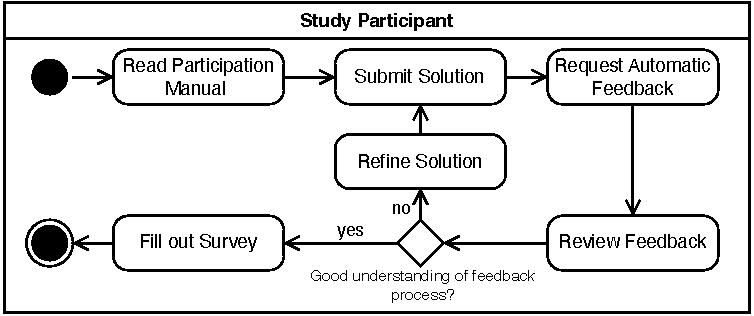
\includegraphics[width=0.6\linewidth]{figures/Study-Design.pdf}
  \caption{UML activity diagram illustrating the study procedure from a participant's perspective.}
  \label{fig:Study-Design}
\end{figure}

Following this hands-on experience, participants were asked to complete a survey hosted on the community version of the open-source survey tool LimeSurvey\footnote{\url{https://www.limesurvey.org}}.
This survey aimed to gather their opinions on direct automated feedback and collect feedback on their overall experience with the feature.
The study employed a mixed methods approach, combining quantitative and qualitative data collection methods.

All survey questions, except for the introductory demographic queries and the five final voluntary free-text responses (\ref{Q18} - \ref{Q22}), employed a 5-point Likert scale \cite{allen:2007:LikertScalesData} ranging from ``strongly agree'' to ``strongly disagree'' and were mandatory. 
The survey questions mapped to the research questions as follows:

%todo: cite nielsen regarding number of participants

\begin{enumerate}[label=\textbf{RQ\arabic*}]
  \item \textbf{Engagement and Motivation}
    \begin{enumerate}[label=\textbf{Q\arabic*},resume,ref=Q\arabic*]
      \item \label{Q1} The direct automated feedback keeps me more engaged in the learning process.
      \item \label{Q2} The direct automatic feedback motivates me to repeatedly improve my code.
      \item \label{Q3} The direct automated feedback makes me feel more motivated to complete my programming assignments.
      \item \label{Q4} The direct automated feedback encourages me to experiment more with my coding solutions.
    \end{enumerate}
  \item \textbf{Comfort with Feedback Source}
  \begin{enumerate}[label=\textbf{Q\arabic*},resume,ref=Q\arabic*]
    \item \label{Q5} I feel more comfortable requesting direct automated feedback than feedback from a human tutor.
    \item \label{Q6} I am likely to request feedback more frequently when using direct automated feedback than feedback from my course professor.
    \item \label{Q7} I find receiving direct automated feedback less intimidating than receiving feedback from a human tutor.
    \item \label{Q8} I feel that requesting direct automated feedback is more convenient than arranging a meeting with a human tutor.
  \end{enumerate}
  \item \textbf{Perceived Effectiveness}
    \begin{enumerate}[label=\textbf{Q\arabic*},resume,ref=Q\arabic*]
      \item \label{Q9} The direct automated feedback helps me understand my mistakes.
      \item \label{Q10} The direct automated feedback is more effective than one-time feedback.
      \item \label{Q11} The direct automated feedback has significantly improved the quality of my programming assignment.
      \item \label{Q12} The direct automated feedback is a helpful addition to the automatic test case results.
      \item \label{Q13} I feel that having access to direct automated feedback continuously helps me more than arranging a meeting with a human tutor.
    \end{enumerate}
  \item \textbf{Usability and Helpfulness}
    \begin{enumerate}[label=\textbf{Q\arabic*},resume,ref=Q\arabic*]
      \item \label{Q14} It is easy to receive direct automated feedback  on my programming assignments.
      \item \label{Q15} I would rather use the direct automated feedback integrated into Artemis than use an external AI tool for getting feedback.
      \item \label{Q16} I find the direct automated feedback helpful in improving my programming skills.
      \item \label{Q17} I am satisfied with the overall performance of the direct automated feedback.
      \item \label{Q18} Are there any improvements that you would suggest for direct automated feedback?
      \item \label{Q19} How did you find the feedback?
      \item \label{Q20} What kind of feedback would you like to receive?
      \item \label{Q21} Was there anything you particularly liked about the direct automated feedback process?
      \item \label{Q22} What difficulties did you encounter when using the direct automated feedback process?
    \end{enumerate}
\end{enumerate}

%todo: Describe free text questions

% %Question Group 1
% The survey commences with a series of introductory demographic inquiries, including the student's current study program, ongoing degree pursued, and academic semester. 
% Additionally, respondents are asked to provide information regarding the hardware employed, including details on the operating system and web browser used.
% The final question in this group asks participants to describe their programming experience.

% %Question Group 2
% Following the demographic section, the survey explores participants' opinions on the impact of direct automated feedback on student engagement and motivation.
% %Question Group 3
% Subsequently, the survey queries participants on their comfort with the feedback source, specifically whether they prefer receiving feedback from a human tutor or from the DAFeeD feature.
% %Question Group 4
% The survey then investigates aspects related to participants' perceived effectiveness of the DAFeeD feature.
% %Question Group 5
% In the final question group, participants assess the overall usability and helpfulness of the DAFeeD feature.


\subsection{Results}

In the following paragraphs, we present the results. 
The answers to each of the Likert scale questions are visualized in Figure \ref{fig:Survey-Results}.

\begin{figure}[htpb]
  \centering
  \resizebox{0.8\textwidth}{!}{
    %% Creator: Matplotlib, PGF backend
%%
%% To include the figure in your LaTeX document, write
%%   \input{<filename>.pgf}
%%
%% Make sure the required packages are loaded in your preamble
%%   \usepackage{pgf}
%%
%% Also ensure that all the required font packages are loaded; for instance,
%% the lmodern package is sometimes necessary when using math font.
%%   \usepackage{lmodern}
%%
%% Figures using additional raster images can only be included by \input if
%% they are in the same directory as the main LaTeX file. For loading figures
%% from other directories you can use the `import` package
%%   \usepackage{import}
%%
%% and then include the figures with
%%   \import{<path to file>}{<filename>.pgf}
%%
%% Matplotlib used the following preamble
%%   \def#1{#1}
%%   \everymath=\expandafter{\the\everymath\displaystyle}
%%   
%%   \makeatletter\@ifpackageloaded{underscore}{}{\usepackage[strings]{underscore}}\makeatother
%%
\begingroup%
\makeatletter%
\begin{pgfpicture}%
\pgfpathrectangle{\pgfpointorigin}{\pgfqpoint{7.071306in}{4.492358in}}%
\pgfusepath{use as bounding box, clip}%
\begin{pgfscope}%
\pgfsetbuttcap%
\pgfsetmiterjoin%
\definecolor{currentfill}{rgb}{1.000000,1.000000,1.000000}%
\pgfsetfillcolor{currentfill}%
\pgfsetlinewidth{0.000000pt}%
\definecolor{currentstroke}{rgb}{1.000000,1.000000,1.000000}%
\pgfsetstrokecolor{currentstroke}%
\pgfsetdash{}{0pt}%
\pgfpathmoveto{\pgfqpoint{0.000000in}{0.000000in}}%
\pgfpathlineto{\pgfqpoint{7.071306in}{0.000000in}}%
\pgfpathlineto{\pgfqpoint{7.071306in}{4.492358in}}%
\pgfpathlineto{\pgfqpoint{0.000000in}{4.492358in}}%
\pgfpathlineto{\pgfqpoint{0.000000in}{0.000000in}}%
\pgfpathclose%
\pgfusepath{fill}%
\end{pgfscope}%
\begin{pgfscope}%
\pgfsetbuttcap%
\pgfsetmiterjoin%
\definecolor{currentfill}{rgb}{1.000000,1.000000,1.000000}%
\pgfsetfillcolor{currentfill}%
\pgfsetlinewidth{0.000000pt}%
\definecolor{currentstroke}{rgb}{0.000000,0.000000,0.000000}%
\pgfsetstrokecolor{currentstroke}%
\pgfsetstrokeopacity{0.000000}%
\pgfsetdash{}{0pt}%
\pgfpathmoveto{\pgfqpoint{2.362505in}{0.393284in}}%
\pgfpathlineto{\pgfqpoint{7.012505in}{0.393284in}}%
\pgfpathlineto{\pgfqpoint{7.012505in}{4.243284in}}%
\pgfpathlineto{\pgfqpoint{2.362505in}{4.243284in}}%
\pgfpathlineto{\pgfqpoint{2.362505in}{0.393284in}}%
\pgfpathclose%
\pgfusepath{fill}%
\end{pgfscope}%
\begin{pgfscope}%
\pgfpathrectangle{\pgfqpoint{2.362505in}{0.393284in}}{\pgfqpoint{4.650000in}{3.850000in}}%
\pgfusepath{clip}%
\pgfsetbuttcap%
\pgfsetmiterjoin%
\definecolor{currentfill}{rgb}{0.843137,0.188235,0.152941}%
\pgfsetfillcolor{currentfill}%
\pgfsetlinewidth{0.000000pt}%
\definecolor{currentstroke}{rgb}{0.000000,0.000000,0.000000}%
\pgfsetstrokecolor{currentstroke}%
\pgfsetstrokeopacity{0.000000}%
\pgfsetdash{}{0pt}%
\pgfpathmoveto{\pgfqpoint{2.362505in}{4.187325in}}%
\pgfpathlineto{\pgfqpoint{2.362505in}{4.187325in}}%
\pgfpathlineto{\pgfqpoint{2.362505in}{4.030639in}}%
\pgfpathlineto{\pgfqpoint{2.362505in}{4.030639in}}%
\pgfpathlineto{\pgfqpoint{2.362505in}{4.187325in}}%
\pgfpathclose%
\pgfusepath{fill}%
\end{pgfscope}%
\begin{pgfscope}%
\pgfpathrectangle{\pgfqpoint{2.362505in}{0.393284in}}{\pgfqpoint{4.650000in}{3.850000in}}%
\pgfusepath{clip}%
\pgfsetbuttcap%
\pgfsetmiterjoin%
\definecolor{currentfill}{rgb}{0.843137,0.188235,0.152941}%
\pgfsetfillcolor{currentfill}%
\pgfsetlinewidth{0.000000pt}%
\definecolor{currentstroke}{rgb}{0.000000,0.000000,0.000000}%
\pgfsetstrokecolor{currentstroke}%
\pgfsetstrokeopacity{0.000000}%
\pgfsetdash{}{0pt}%
\pgfpathmoveto{\pgfqpoint{2.362505in}{3.963487in}}%
\pgfpathlineto{\pgfqpoint{2.362505in}{3.963487in}}%
\pgfpathlineto{\pgfqpoint{2.362505in}{3.806801in}}%
\pgfpathlineto{\pgfqpoint{2.362505in}{3.806801in}}%
\pgfpathlineto{\pgfqpoint{2.362505in}{3.963487in}}%
\pgfpathclose%
\pgfusepath{fill}%
\end{pgfscope}%
\begin{pgfscope}%
\pgfpathrectangle{\pgfqpoint{2.362505in}{0.393284in}}{\pgfqpoint{4.650000in}{3.850000in}}%
\pgfusepath{clip}%
\pgfsetbuttcap%
\pgfsetmiterjoin%
\definecolor{currentfill}{rgb}{0.843137,0.188235,0.152941}%
\pgfsetfillcolor{currentfill}%
\pgfsetlinewidth{0.000000pt}%
\definecolor{currentstroke}{rgb}{0.000000,0.000000,0.000000}%
\pgfsetstrokecolor{currentstroke}%
\pgfsetstrokeopacity{0.000000}%
\pgfsetdash{}{0pt}%
\pgfpathmoveto{\pgfqpoint{2.362505in}{3.739650in}}%
\pgfpathlineto{\pgfqpoint{2.362505in}{3.739650in}}%
\pgfpathlineto{\pgfqpoint{2.362505in}{3.582964in}}%
\pgfpathlineto{\pgfqpoint{2.362505in}{3.582964in}}%
\pgfpathlineto{\pgfqpoint{2.362505in}{3.739650in}}%
\pgfpathclose%
\pgfusepath{fill}%
\end{pgfscope}%
\begin{pgfscope}%
\pgfpathrectangle{\pgfqpoint{2.362505in}{0.393284in}}{\pgfqpoint{4.650000in}{3.850000in}}%
\pgfusepath{clip}%
\pgfsetbuttcap%
\pgfsetmiterjoin%
\definecolor{currentfill}{rgb}{0.843137,0.188235,0.152941}%
\pgfsetfillcolor{currentfill}%
\pgfsetlinewidth{0.000000pt}%
\definecolor{currentstroke}{rgb}{0.000000,0.000000,0.000000}%
\pgfsetstrokecolor{currentstroke}%
\pgfsetstrokeopacity{0.000000}%
\pgfsetdash{}{0pt}%
\pgfpathmoveto{\pgfqpoint{2.362505in}{3.515813in}}%
\pgfpathlineto{\pgfqpoint{2.595005in}{3.515813in}}%
\pgfpathlineto{\pgfqpoint{2.595005in}{3.359127in}}%
\pgfpathlineto{\pgfqpoint{2.362505in}{3.359127in}}%
\pgfpathlineto{\pgfqpoint{2.362505in}{3.515813in}}%
\pgfpathclose%
\pgfusepath{fill}%
\end{pgfscope}%
\begin{pgfscope}%
\pgfpathrectangle{\pgfqpoint{2.362505in}{0.393284in}}{\pgfqpoint{4.650000in}{3.850000in}}%
\pgfusepath{clip}%
\pgfsetbuttcap%
\pgfsetmiterjoin%
\definecolor{currentfill}{rgb}{0.843137,0.188235,0.152941}%
\pgfsetfillcolor{currentfill}%
\pgfsetlinewidth{0.000000pt}%
\definecolor{currentstroke}{rgb}{0.000000,0.000000,0.000000}%
\pgfsetstrokecolor{currentstroke}%
\pgfsetstrokeopacity{0.000000}%
\pgfsetdash{}{0pt}%
\pgfpathmoveto{\pgfqpoint{2.362505in}{3.291976in}}%
\pgfpathlineto{\pgfqpoint{2.362505in}{3.291976in}}%
\pgfpathlineto{\pgfqpoint{2.362505in}{3.135290in}}%
\pgfpathlineto{\pgfqpoint{2.362505in}{3.135290in}}%
\pgfpathlineto{\pgfqpoint{2.362505in}{3.291976in}}%
\pgfpathclose%
\pgfusepath{fill}%
\end{pgfscope}%
\begin{pgfscope}%
\pgfpathrectangle{\pgfqpoint{2.362505in}{0.393284in}}{\pgfqpoint{4.650000in}{3.850000in}}%
\pgfusepath{clip}%
\pgfsetbuttcap%
\pgfsetmiterjoin%
\definecolor{currentfill}{rgb}{0.843137,0.188235,0.152941}%
\pgfsetfillcolor{currentfill}%
\pgfsetlinewidth{0.000000pt}%
\definecolor{currentstroke}{rgb}{0.000000,0.000000,0.000000}%
\pgfsetstrokecolor{currentstroke}%
\pgfsetstrokeopacity{0.000000}%
\pgfsetdash{}{0pt}%
\pgfpathmoveto{\pgfqpoint{2.362505in}{3.068139in}}%
\pgfpathlineto{\pgfqpoint{2.362505in}{3.068139in}}%
\pgfpathlineto{\pgfqpoint{2.362505in}{2.911452in}}%
\pgfpathlineto{\pgfqpoint{2.362505in}{2.911452in}}%
\pgfpathlineto{\pgfqpoint{2.362505in}{3.068139in}}%
\pgfpathclose%
\pgfusepath{fill}%
\end{pgfscope}%
\begin{pgfscope}%
\pgfpathrectangle{\pgfqpoint{2.362505in}{0.393284in}}{\pgfqpoint{4.650000in}{3.850000in}}%
\pgfusepath{clip}%
\pgfsetbuttcap%
\pgfsetmiterjoin%
\definecolor{currentfill}{rgb}{0.843137,0.188235,0.152941}%
\pgfsetfillcolor{currentfill}%
\pgfsetlinewidth{0.000000pt}%
\definecolor{currentstroke}{rgb}{0.000000,0.000000,0.000000}%
\pgfsetstrokecolor{currentstroke}%
\pgfsetstrokeopacity{0.000000}%
\pgfsetdash{}{0pt}%
\pgfpathmoveto{\pgfqpoint{2.362505in}{2.844301in}}%
\pgfpathlineto{\pgfqpoint{2.362505in}{2.844301in}}%
\pgfpathlineto{\pgfqpoint{2.362505in}{2.687615in}}%
\pgfpathlineto{\pgfqpoint{2.362505in}{2.687615in}}%
\pgfpathlineto{\pgfqpoint{2.362505in}{2.844301in}}%
\pgfpathclose%
\pgfusepath{fill}%
\end{pgfscope}%
\begin{pgfscope}%
\pgfpathrectangle{\pgfqpoint{2.362505in}{0.393284in}}{\pgfqpoint{4.650000in}{3.850000in}}%
\pgfusepath{clip}%
\pgfsetbuttcap%
\pgfsetmiterjoin%
\definecolor{currentfill}{rgb}{0.843137,0.188235,0.152941}%
\pgfsetfillcolor{currentfill}%
\pgfsetlinewidth{0.000000pt}%
\definecolor{currentstroke}{rgb}{0.000000,0.000000,0.000000}%
\pgfsetstrokecolor{currentstroke}%
\pgfsetstrokeopacity{0.000000}%
\pgfsetdash{}{0pt}%
\pgfpathmoveto{\pgfqpoint{2.362505in}{2.620464in}}%
\pgfpathlineto{\pgfqpoint{2.362505in}{2.620464in}}%
\pgfpathlineto{\pgfqpoint{2.362505in}{2.463778in}}%
\pgfpathlineto{\pgfqpoint{2.362505in}{2.463778in}}%
\pgfpathlineto{\pgfqpoint{2.362505in}{2.620464in}}%
\pgfpathclose%
\pgfusepath{fill}%
\end{pgfscope}%
\begin{pgfscope}%
\pgfpathrectangle{\pgfqpoint{2.362505in}{0.393284in}}{\pgfqpoint{4.650000in}{3.850000in}}%
\pgfusepath{clip}%
\pgfsetbuttcap%
\pgfsetmiterjoin%
\definecolor{currentfill}{rgb}{0.843137,0.188235,0.152941}%
\pgfsetfillcolor{currentfill}%
\pgfsetlinewidth{0.000000pt}%
\definecolor{currentstroke}{rgb}{0.000000,0.000000,0.000000}%
\pgfsetstrokecolor{currentstroke}%
\pgfsetstrokeopacity{0.000000}%
\pgfsetdash{}{0pt}%
\pgfpathmoveto{\pgfqpoint{2.362505in}{2.396627in}}%
\pgfpathlineto{\pgfqpoint{2.362505in}{2.396627in}}%
\pgfpathlineto{\pgfqpoint{2.362505in}{2.239941in}}%
\pgfpathlineto{\pgfqpoint{2.362505in}{2.239941in}}%
\pgfpathlineto{\pgfqpoint{2.362505in}{2.396627in}}%
\pgfpathclose%
\pgfusepath{fill}%
\end{pgfscope}%
\begin{pgfscope}%
\pgfpathrectangle{\pgfqpoint{2.362505in}{0.393284in}}{\pgfqpoint{4.650000in}{3.850000in}}%
\pgfusepath{clip}%
\pgfsetbuttcap%
\pgfsetmiterjoin%
\definecolor{currentfill}{rgb}{0.843137,0.188235,0.152941}%
\pgfsetfillcolor{currentfill}%
\pgfsetlinewidth{0.000000pt}%
\definecolor{currentstroke}{rgb}{0.000000,0.000000,0.000000}%
\pgfsetstrokecolor{currentstroke}%
\pgfsetstrokeopacity{0.000000}%
\pgfsetdash{}{0pt}%
\pgfpathmoveto{\pgfqpoint{2.362505in}{2.172790in}}%
\pgfpathlineto{\pgfqpoint{2.362505in}{2.172790in}}%
\pgfpathlineto{\pgfqpoint{2.362505in}{2.016104in}}%
\pgfpathlineto{\pgfqpoint{2.362505in}{2.016104in}}%
\pgfpathlineto{\pgfqpoint{2.362505in}{2.172790in}}%
\pgfpathclose%
\pgfusepath{fill}%
\end{pgfscope}%
\begin{pgfscope}%
\pgfpathrectangle{\pgfqpoint{2.362505in}{0.393284in}}{\pgfqpoint{4.650000in}{3.850000in}}%
\pgfusepath{clip}%
\pgfsetbuttcap%
\pgfsetmiterjoin%
\definecolor{currentfill}{rgb}{0.843137,0.188235,0.152941}%
\pgfsetfillcolor{currentfill}%
\pgfsetlinewidth{0.000000pt}%
\definecolor{currentstroke}{rgb}{0.000000,0.000000,0.000000}%
\pgfsetstrokecolor{currentstroke}%
\pgfsetstrokeopacity{0.000000}%
\pgfsetdash{}{0pt}%
\pgfpathmoveto{\pgfqpoint{2.362505in}{1.948952in}}%
\pgfpathlineto{\pgfqpoint{2.362505in}{1.948952in}}%
\pgfpathlineto{\pgfqpoint{2.362505in}{1.792266in}}%
\pgfpathlineto{\pgfqpoint{2.362505in}{1.792266in}}%
\pgfpathlineto{\pgfqpoint{2.362505in}{1.948952in}}%
\pgfpathclose%
\pgfusepath{fill}%
\end{pgfscope}%
\begin{pgfscope}%
\pgfpathrectangle{\pgfqpoint{2.362505in}{0.393284in}}{\pgfqpoint{4.650000in}{3.850000in}}%
\pgfusepath{clip}%
\pgfsetbuttcap%
\pgfsetmiterjoin%
\definecolor{currentfill}{rgb}{0.843137,0.188235,0.152941}%
\pgfsetfillcolor{currentfill}%
\pgfsetlinewidth{0.000000pt}%
\definecolor{currentstroke}{rgb}{0.000000,0.000000,0.000000}%
\pgfsetstrokecolor{currentstroke}%
\pgfsetstrokeopacity{0.000000}%
\pgfsetdash{}{0pt}%
\pgfpathmoveto{\pgfqpoint{2.362505in}{1.725115in}}%
\pgfpathlineto{\pgfqpoint{2.362505in}{1.725115in}}%
\pgfpathlineto{\pgfqpoint{2.362505in}{1.568429in}}%
\pgfpathlineto{\pgfqpoint{2.362505in}{1.568429in}}%
\pgfpathlineto{\pgfqpoint{2.362505in}{1.725115in}}%
\pgfpathclose%
\pgfusepath{fill}%
\end{pgfscope}%
\begin{pgfscope}%
\pgfpathrectangle{\pgfqpoint{2.362505in}{0.393284in}}{\pgfqpoint{4.650000in}{3.850000in}}%
\pgfusepath{clip}%
\pgfsetbuttcap%
\pgfsetmiterjoin%
\definecolor{currentfill}{rgb}{0.843137,0.188235,0.152941}%
\pgfsetfillcolor{currentfill}%
\pgfsetlinewidth{0.000000pt}%
\definecolor{currentstroke}{rgb}{0.000000,0.000000,0.000000}%
\pgfsetstrokecolor{currentstroke}%
\pgfsetstrokeopacity{0.000000}%
\pgfsetdash{}{0pt}%
\pgfpathmoveto{\pgfqpoint{2.362505in}{1.501278in}}%
\pgfpathlineto{\pgfqpoint{2.362505in}{1.501278in}}%
\pgfpathlineto{\pgfqpoint{2.362505in}{1.344592in}}%
\pgfpathlineto{\pgfqpoint{2.362505in}{1.344592in}}%
\pgfpathlineto{\pgfqpoint{2.362505in}{1.501278in}}%
\pgfpathclose%
\pgfusepath{fill}%
\end{pgfscope}%
\begin{pgfscope}%
\pgfpathrectangle{\pgfqpoint{2.362505in}{0.393284in}}{\pgfqpoint{4.650000in}{3.850000in}}%
\pgfusepath{clip}%
\pgfsetbuttcap%
\pgfsetmiterjoin%
\definecolor{currentfill}{rgb}{0.843137,0.188235,0.152941}%
\pgfsetfillcolor{currentfill}%
\pgfsetlinewidth{0.000000pt}%
\definecolor{currentstroke}{rgb}{0.000000,0.000000,0.000000}%
\pgfsetstrokecolor{currentstroke}%
\pgfsetstrokeopacity{0.000000}%
\pgfsetdash{}{0pt}%
\pgfpathmoveto{\pgfqpoint{2.362505in}{1.277441in}}%
\pgfpathlineto{\pgfqpoint{2.362505in}{1.277441in}}%
\pgfpathlineto{\pgfqpoint{2.362505in}{1.120755in}}%
\pgfpathlineto{\pgfqpoint{2.362505in}{1.120755in}}%
\pgfpathlineto{\pgfqpoint{2.362505in}{1.277441in}}%
\pgfpathclose%
\pgfusepath{fill}%
\end{pgfscope}%
\begin{pgfscope}%
\pgfpathrectangle{\pgfqpoint{2.362505in}{0.393284in}}{\pgfqpoint{4.650000in}{3.850000in}}%
\pgfusepath{clip}%
\pgfsetbuttcap%
\pgfsetmiterjoin%
\definecolor{currentfill}{rgb}{0.843137,0.188235,0.152941}%
\pgfsetfillcolor{currentfill}%
\pgfsetlinewidth{0.000000pt}%
\definecolor{currentstroke}{rgb}{0.000000,0.000000,0.000000}%
\pgfsetstrokecolor{currentstroke}%
\pgfsetstrokeopacity{0.000000}%
\pgfsetdash{}{0pt}%
\pgfpathmoveto{\pgfqpoint{2.362505in}{1.053604in}}%
\pgfpathlineto{\pgfqpoint{2.362505in}{1.053604in}}%
\pgfpathlineto{\pgfqpoint{2.362505in}{0.896918in}}%
\pgfpathlineto{\pgfqpoint{2.362505in}{0.896918in}}%
\pgfpathlineto{\pgfqpoint{2.362505in}{1.053604in}}%
\pgfpathclose%
\pgfusepath{fill}%
\end{pgfscope}%
\begin{pgfscope}%
\pgfpathrectangle{\pgfqpoint{2.362505in}{0.393284in}}{\pgfqpoint{4.650000in}{3.850000in}}%
\pgfusepath{clip}%
\pgfsetbuttcap%
\pgfsetmiterjoin%
\definecolor{currentfill}{rgb}{0.843137,0.188235,0.152941}%
\pgfsetfillcolor{currentfill}%
\pgfsetlinewidth{0.000000pt}%
\definecolor{currentstroke}{rgb}{0.000000,0.000000,0.000000}%
\pgfsetstrokecolor{currentstroke}%
\pgfsetstrokeopacity{0.000000}%
\pgfsetdash{}{0pt}%
\pgfpathmoveto{\pgfqpoint{2.362505in}{0.829766in}}%
\pgfpathlineto{\pgfqpoint{2.362505in}{0.829766in}}%
\pgfpathlineto{\pgfqpoint{2.362505in}{0.673080in}}%
\pgfpathlineto{\pgfqpoint{2.362505in}{0.673080in}}%
\pgfpathlineto{\pgfqpoint{2.362505in}{0.829766in}}%
\pgfpathclose%
\pgfusepath{fill}%
\end{pgfscope}%
\begin{pgfscope}%
\pgfpathrectangle{\pgfqpoint{2.362505in}{0.393284in}}{\pgfqpoint{4.650000in}{3.850000in}}%
\pgfusepath{clip}%
\pgfsetbuttcap%
\pgfsetmiterjoin%
\definecolor{currentfill}{rgb}{0.843137,0.188235,0.152941}%
\pgfsetfillcolor{currentfill}%
\pgfsetlinewidth{0.000000pt}%
\definecolor{currentstroke}{rgb}{0.000000,0.000000,0.000000}%
\pgfsetstrokecolor{currentstroke}%
\pgfsetstrokeopacity{0.000000}%
\pgfsetdash{}{0pt}%
\pgfpathmoveto{\pgfqpoint{2.362505in}{0.605929in}}%
\pgfpathlineto{\pgfqpoint{2.362505in}{0.605929in}}%
\pgfpathlineto{\pgfqpoint{2.362505in}{0.449243in}}%
\pgfpathlineto{\pgfqpoint{2.362505in}{0.449243in}}%
\pgfpathlineto{\pgfqpoint{2.362505in}{0.605929in}}%
\pgfpathclose%
\pgfusepath{fill}%
\end{pgfscope}%
\begin{pgfscope}%
\pgfpathrectangle{\pgfqpoint{2.362505in}{0.393284in}}{\pgfqpoint{4.650000in}{3.850000in}}%
\pgfusepath{clip}%
\pgfsetbuttcap%
\pgfsetmiterjoin%
\definecolor{currentfill}{rgb}{0.988235,0.552941,0.349020}%
\pgfsetfillcolor{currentfill}%
\pgfsetlinewidth{0.000000pt}%
\definecolor{currentstroke}{rgb}{0.000000,0.000000,0.000000}%
\pgfsetstrokecolor{currentstroke}%
\pgfsetstrokeopacity{0.000000}%
\pgfsetdash{}{0pt}%
\pgfpathmoveto{\pgfqpoint{2.362505in}{4.187325in}}%
\pgfpathlineto{\pgfqpoint{2.362505in}{4.187325in}}%
\pgfpathlineto{\pgfqpoint{2.362505in}{4.030639in}}%
\pgfpathlineto{\pgfqpoint{2.362505in}{4.030639in}}%
\pgfpathlineto{\pgfqpoint{2.362505in}{4.187325in}}%
\pgfpathclose%
\pgfusepath{fill}%
\end{pgfscope}%
\begin{pgfscope}%
\pgfpathrectangle{\pgfqpoint{2.362505in}{0.393284in}}{\pgfqpoint{4.650000in}{3.850000in}}%
\pgfusepath{clip}%
\pgfsetbuttcap%
\pgfsetmiterjoin%
\definecolor{currentfill}{rgb}{0.988235,0.552941,0.349020}%
\pgfsetfillcolor{currentfill}%
\pgfsetlinewidth{0.000000pt}%
\definecolor{currentstroke}{rgb}{0.000000,0.000000,0.000000}%
\pgfsetstrokecolor{currentstroke}%
\pgfsetstrokeopacity{0.000000}%
\pgfsetdash{}{0pt}%
\pgfpathmoveto{\pgfqpoint{2.362505in}{3.963487in}}%
\pgfpathlineto{\pgfqpoint{2.595005in}{3.963487in}}%
\pgfpathlineto{\pgfqpoint{2.595005in}{3.806801in}}%
\pgfpathlineto{\pgfqpoint{2.362505in}{3.806801in}}%
\pgfpathlineto{\pgfqpoint{2.362505in}{3.963487in}}%
\pgfpathclose%
\pgfusepath{fill}%
\end{pgfscope}%
\begin{pgfscope}%
\pgfpathrectangle{\pgfqpoint{2.362505in}{0.393284in}}{\pgfqpoint{4.650000in}{3.850000in}}%
\pgfusepath{clip}%
\pgfsetbuttcap%
\pgfsetmiterjoin%
\definecolor{currentfill}{rgb}{0.988235,0.552941,0.349020}%
\pgfsetfillcolor{currentfill}%
\pgfsetlinewidth{0.000000pt}%
\definecolor{currentstroke}{rgb}{0.000000,0.000000,0.000000}%
\pgfsetstrokecolor{currentstroke}%
\pgfsetstrokeopacity{0.000000}%
\pgfsetdash{}{0pt}%
\pgfpathmoveto{\pgfqpoint{2.362505in}{3.739650in}}%
\pgfpathlineto{\pgfqpoint{2.595005in}{3.739650in}}%
\pgfpathlineto{\pgfqpoint{2.595005in}{3.582964in}}%
\pgfpathlineto{\pgfqpoint{2.362505in}{3.582964in}}%
\pgfpathlineto{\pgfqpoint{2.362505in}{3.739650in}}%
\pgfpathclose%
\pgfusepath{fill}%
\end{pgfscope}%
\begin{pgfscope}%
\pgfpathrectangle{\pgfqpoint{2.362505in}{0.393284in}}{\pgfqpoint{4.650000in}{3.850000in}}%
\pgfusepath{clip}%
\pgfsetbuttcap%
\pgfsetmiterjoin%
\definecolor{currentfill}{rgb}{0.988235,0.552941,0.349020}%
\pgfsetfillcolor{currentfill}%
\pgfsetlinewidth{0.000000pt}%
\definecolor{currentstroke}{rgb}{0.000000,0.000000,0.000000}%
\pgfsetstrokecolor{currentstroke}%
\pgfsetstrokeopacity{0.000000}%
\pgfsetdash{}{0pt}%
\pgfpathmoveto{\pgfqpoint{2.595005in}{3.515813in}}%
\pgfpathlineto{\pgfqpoint{2.827505in}{3.515813in}}%
\pgfpathlineto{\pgfqpoint{2.827505in}{3.359127in}}%
\pgfpathlineto{\pgfqpoint{2.595005in}{3.359127in}}%
\pgfpathlineto{\pgfqpoint{2.595005in}{3.515813in}}%
\pgfpathclose%
\pgfusepath{fill}%
\end{pgfscope}%
\begin{pgfscope}%
\pgfpathrectangle{\pgfqpoint{2.362505in}{0.393284in}}{\pgfqpoint{4.650000in}{3.850000in}}%
\pgfusepath{clip}%
\pgfsetbuttcap%
\pgfsetmiterjoin%
\definecolor{currentfill}{rgb}{0.988235,0.552941,0.349020}%
\pgfsetfillcolor{currentfill}%
\pgfsetlinewidth{0.000000pt}%
\definecolor{currentstroke}{rgb}{0.000000,0.000000,0.000000}%
\pgfsetstrokecolor{currentstroke}%
\pgfsetstrokeopacity{0.000000}%
\pgfsetdash{}{0pt}%
\pgfpathmoveto{\pgfqpoint{2.362505in}{3.291976in}}%
\pgfpathlineto{\pgfqpoint{2.362505in}{3.291976in}}%
\pgfpathlineto{\pgfqpoint{2.362505in}{3.135290in}}%
\pgfpathlineto{\pgfqpoint{2.362505in}{3.135290in}}%
\pgfpathlineto{\pgfqpoint{2.362505in}{3.291976in}}%
\pgfpathclose%
\pgfusepath{fill}%
\end{pgfscope}%
\begin{pgfscope}%
\pgfpathrectangle{\pgfqpoint{2.362505in}{0.393284in}}{\pgfqpoint{4.650000in}{3.850000in}}%
\pgfusepath{clip}%
\pgfsetbuttcap%
\pgfsetmiterjoin%
\definecolor{currentfill}{rgb}{0.988235,0.552941,0.349020}%
\pgfsetfillcolor{currentfill}%
\pgfsetlinewidth{0.000000pt}%
\definecolor{currentstroke}{rgb}{0.000000,0.000000,0.000000}%
\pgfsetstrokecolor{currentstroke}%
\pgfsetstrokeopacity{0.000000}%
\pgfsetdash{}{0pt}%
\pgfpathmoveto{\pgfqpoint{2.362505in}{3.068139in}}%
\pgfpathlineto{\pgfqpoint{2.362505in}{3.068139in}}%
\pgfpathlineto{\pgfqpoint{2.362505in}{2.911452in}}%
\pgfpathlineto{\pgfqpoint{2.362505in}{2.911452in}}%
\pgfpathlineto{\pgfqpoint{2.362505in}{3.068139in}}%
\pgfpathclose%
\pgfusepath{fill}%
\end{pgfscope}%
\begin{pgfscope}%
\pgfpathrectangle{\pgfqpoint{2.362505in}{0.393284in}}{\pgfqpoint{4.650000in}{3.850000in}}%
\pgfusepath{clip}%
\pgfsetbuttcap%
\pgfsetmiterjoin%
\definecolor{currentfill}{rgb}{0.988235,0.552941,0.349020}%
\pgfsetfillcolor{currentfill}%
\pgfsetlinewidth{0.000000pt}%
\definecolor{currentstroke}{rgb}{0.000000,0.000000,0.000000}%
\pgfsetstrokecolor{currentstroke}%
\pgfsetstrokeopacity{0.000000}%
\pgfsetdash{}{0pt}%
\pgfpathmoveto{\pgfqpoint{2.362505in}{2.844301in}}%
\pgfpathlineto{\pgfqpoint{2.827505in}{2.844301in}}%
\pgfpathlineto{\pgfqpoint{2.827505in}{2.687615in}}%
\pgfpathlineto{\pgfqpoint{2.362505in}{2.687615in}}%
\pgfpathlineto{\pgfqpoint{2.362505in}{2.844301in}}%
\pgfpathclose%
\pgfusepath{fill}%
\end{pgfscope}%
\begin{pgfscope}%
\pgfpathrectangle{\pgfqpoint{2.362505in}{0.393284in}}{\pgfqpoint{4.650000in}{3.850000in}}%
\pgfusepath{clip}%
\pgfsetbuttcap%
\pgfsetmiterjoin%
\definecolor{currentfill}{rgb}{0.988235,0.552941,0.349020}%
\pgfsetfillcolor{currentfill}%
\pgfsetlinewidth{0.000000pt}%
\definecolor{currentstroke}{rgb}{0.000000,0.000000,0.000000}%
\pgfsetstrokecolor{currentstroke}%
\pgfsetstrokeopacity{0.000000}%
\pgfsetdash{}{0pt}%
\pgfpathmoveto{\pgfqpoint{2.362505in}{2.620464in}}%
\pgfpathlineto{\pgfqpoint{2.362505in}{2.620464in}}%
\pgfpathlineto{\pgfqpoint{2.362505in}{2.463778in}}%
\pgfpathlineto{\pgfqpoint{2.362505in}{2.463778in}}%
\pgfpathlineto{\pgfqpoint{2.362505in}{2.620464in}}%
\pgfpathclose%
\pgfusepath{fill}%
\end{pgfscope}%
\begin{pgfscope}%
\pgfpathrectangle{\pgfqpoint{2.362505in}{0.393284in}}{\pgfqpoint{4.650000in}{3.850000in}}%
\pgfusepath{clip}%
\pgfsetbuttcap%
\pgfsetmiterjoin%
\definecolor{currentfill}{rgb}{0.988235,0.552941,0.349020}%
\pgfsetfillcolor{currentfill}%
\pgfsetlinewidth{0.000000pt}%
\definecolor{currentstroke}{rgb}{0.000000,0.000000,0.000000}%
\pgfsetstrokecolor{currentstroke}%
\pgfsetstrokeopacity{0.000000}%
\pgfsetdash{}{0pt}%
\pgfpathmoveto{\pgfqpoint{2.362505in}{2.396627in}}%
\pgfpathlineto{\pgfqpoint{2.362505in}{2.396627in}}%
\pgfpathlineto{\pgfqpoint{2.362505in}{2.239941in}}%
\pgfpathlineto{\pgfqpoint{2.362505in}{2.239941in}}%
\pgfpathlineto{\pgfqpoint{2.362505in}{2.396627in}}%
\pgfpathclose%
\pgfusepath{fill}%
\end{pgfscope}%
\begin{pgfscope}%
\pgfpathrectangle{\pgfqpoint{2.362505in}{0.393284in}}{\pgfqpoint{4.650000in}{3.850000in}}%
\pgfusepath{clip}%
\pgfsetbuttcap%
\pgfsetmiterjoin%
\definecolor{currentfill}{rgb}{0.988235,0.552941,0.349020}%
\pgfsetfillcolor{currentfill}%
\pgfsetlinewidth{0.000000pt}%
\definecolor{currentstroke}{rgb}{0.000000,0.000000,0.000000}%
\pgfsetstrokecolor{currentstroke}%
\pgfsetstrokeopacity{0.000000}%
\pgfsetdash{}{0pt}%
\pgfpathmoveto{\pgfqpoint{2.362505in}{2.172790in}}%
\pgfpathlineto{\pgfqpoint{2.362505in}{2.172790in}}%
\pgfpathlineto{\pgfqpoint{2.362505in}{2.016104in}}%
\pgfpathlineto{\pgfqpoint{2.362505in}{2.016104in}}%
\pgfpathlineto{\pgfqpoint{2.362505in}{2.172790in}}%
\pgfpathclose%
\pgfusepath{fill}%
\end{pgfscope}%
\begin{pgfscope}%
\pgfpathrectangle{\pgfqpoint{2.362505in}{0.393284in}}{\pgfqpoint{4.650000in}{3.850000in}}%
\pgfusepath{clip}%
\pgfsetbuttcap%
\pgfsetmiterjoin%
\definecolor{currentfill}{rgb}{0.988235,0.552941,0.349020}%
\pgfsetfillcolor{currentfill}%
\pgfsetlinewidth{0.000000pt}%
\definecolor{currentstroke}{rgb}{0.000000,0.000000,0.000000}%
\pgfsetstrokecolor{currentstroke}%
\pgfsetstrokeopacity{0.000000}%
\pgfsetdash{}{0pt}%
\pgfpathmoveto{\pgfqpoint{2.362505in}{1.948952in}}%
\pgfpathlineto{\pgfqpoint{2.827505in}{1.948952in}}%
\pgfpathlineto{\pgfqpoint{2.827505in}{1.792266in}}%
\pgfpathlineto{\pgfqpoint{2.362505in}{1.792266in}}%
\pgfpathlineto{\pgfqpoint{2.362505in}{1.948952in}}%
\pgfpathclose%
\pgfusepath{fill}%
\end{pgfscope}%
\begin{pgfscope}%
\pgfpathrectangle{\pgfqpoint{2.362505in}{0.393284in}}{\pgfqpoint{4.650000in}{3.850000in}}%
\pgfusepath{clip}%
\pgfsetbuttcap%
\pgfsetmiterjoin%
\definecolor{currentfill}{rgb}{0.988235,0.552941,0.349020}%
\pgfsetfillcolor{currentfill}%
\pgfsetlinewidth{0.000000pt}%
\definecolor{currentstroke}{rgb}{0.000000,0.000000,0.000000}%
\pgfsetstrokecolor{currentstroke}%
\pgfsetstrokeopacity{0.000000}%
\pgfsetdash{}{0pt}%
\pgfpathmoveto{\pgfqpoint{2.362505in}{1.725115in}}%
\pgfpathlineto{\pgfqpoint{2.362505in}{1.725115in}}%
\pgfpathlineto{\pgfqpoint{2.362505in}{1.568429in}}%
\pgfpathlineto{\pgfqpoint{2.362505in}{1.568429in}}%
\pgfpathlineto{\pgfqpoint{2.362505in}{1.725115in}}%
\pgfpathclose%
\pgfusepath{fill}%
\end{pgfscope}%
\begin{pgfscope}%
\pgfpathrectangle{\pgfqpoint{2.362505in}{0.393284in}}{\pgfqpoint{4.650000in}{3.850000in}}%
\pgfusepath{clip}%
\pgfsetbuttcap%
\pgfsetmiterjoin%
\definecolor{currentfill}{rgb}{0.988235,0.552941,0.349020}%
\pgfsetfillcolor{currentfill}%
\pgfsetlinewidth{0.000000pt}%
\definecolor{currentstroke}{rgb}{0.000000,0.000000,0.000000}%
\pgfsetstrokecolor{currentstroke}%
\pgfsetstrokeopacity{0.000000}%
\pgfsetdash{}{0pt}%
\pgfpathmoveto{\pgfqpoint{2.362505in}{1.501278in}}%
\pgfpathlineto{\pgfqpoint{2.827505in}{1.501278in}}%
\pgfpathlineto{\pgfqpoint{2.827505in}{1.344592in}}%
\pgfpathlineto{\pgfqpoint{2.362505in}{1.344592in}}%
\pgfpathlineto{\pgfqpoint{2.362505in}{1.501278in}}%
\pgfpathclose%
\pgfusepath{fill}%
\end{pgfscope}%
\begin{pgfscope}%
\pgfpathrectangle{\pgfqpoint{2.362505in}{0.393284in}}{\pgfqpoint{4.650000in}{3.850000in}}%
\pgfusepath{clip}%
\pgfsetbuttcap%
\pgfsetmiterjoin%
\definecolor{currentfill}{rgb}{0.988235,0.552941,0.349020}%
\pgfsetfillcolor{currentfill}%
\pgfsetlinewidth{0.000000pt}%
\definecolor{currentstroke}{rgb}{0.000000,0.000000,0.000000}%
\pgfsetstrokecolor{currentstroke}%
\pgfsetstrokeopacity{0.000000}%
\pgfsetdash{}{0pt}%
\pgfpathmoveto{\pgfqpoint{2.362505in}{1.277441in}}%
\pgfpathlineto{\pgfqpoint{2.362505in}{1.277441in}}%
\pgfpathlineto{\pgfqpoint{2.362505in}{1.120755in}}%
\pgfpathlineto{\pgfqpoint{2.362505in}{1.120755in}}%
\pgfpathlineto{\pgfqpoint{2.362505in}{1.277441in}}%
\pgfpathclose%
\pgfusepath{fill}%
\end{pgfscope}%
\begin{pgfscope}%
\pgfpathrectangle{\pgfqpoint{2.362505in}{0.393284in}}{\pgfqpoint{4.650000in}{3.850000in}}%
\pgfusepath{clip}%
\pgfsetbuttcap%
\pgfsetmiterjoin%
\definecolor{currentfill}{rgb}{0.988235,0.552941,0.349020}%
\pgfsetfillcolor{currentfill}%
\pgfsetlinewidth{0.000000pt}%
\definecolor{currentstroke}{rgb}{0.000000,0.000000,0.000000}%
\pgfsetstrokecolor{currentstroke}%
\pgfsetstrokeopacity{0.000000}%
\pgfsetdash{}{0pt}%
\pgfpathmoveto{\pgfqpoint{2.362505in}{1.053604in}}%
\pgfpathlineto{\pgfqpoint{2.595005in}{1.053604in}}%
\pgfpathlineto{\pgfqpoint{2.595005in}{0.896918in}}%
\pgfpathlineto{\pgfqpoint{2.362505in}{0.896918in}}%
\pgfpathlineto{\pgfqpoint{2.362505in}{1.053604in}}%
\pgfpathclose%
\pgfusepath{fill}%
\end{pgfscope}%
\begin{pgfscope}%
\pgfpathrectangle{\pgfqpoint{2.362505in}{0.393284in}}{\pgfqpoint{4.650000in}{3.850000in}}%
\pgfusepath{clip}%
\pgfsetbuttcap%
\pgfsetmiterjoin%
\definecolor{currentfill}{rgb}{0.988235,0.552941,0.349020}%
\pgfsetfillcolor{currentfill}%
\pgfsetlinewidth{0.000000pt}%
\definecolor{currentstroke}{rgb}{0.000000,0.000000,0.000000}%
\pgfsetstrokecolor{currentstroke}%
\pgfsetstrokeopacity{0.000000}%
\pgfsetdash{}{0pt}%
\pgfpathmoveto{\pgfqpoint{2.362505in}{0.829766in}}%
\pgfpathlineto{\pgfqpoint{2.595005in}{0.829766in}}%
\pgfpathlineto{\pgfqpoint{2.595005in}{0.673080in}}%
\pgfpathlineto{\pgfqpoint{2.362505in}{0.673080in}}%
\pgfpathlineto{\pgfqpoint{2.362505in}{0.829766in}}%
\pgfpathclose%
\pgfusepath{fill}%
\end{pgfscope}%
\begin{pgfscope}%
\pgfpathrectangle{\pgfqpoint{2.362505in}{0.393284in}}{\pgfqpoint{4.650000in}{3.850000in}}%
\pgfusepath{clip}%
\pgfsetbuttcap%
\pgfsetmiterjoin%
\definecolor{currentfill}{rgb}{0.988235,0.552941,0.349020}%
\pgfsetfillcolor{currentfill}%
\pgfsetlinewidth{0.000000pt}%
\definecolor{currentstroke}{rgb}{0.000000,0.000000,0.000000}%
\pgfsetstrokecolor{currentstroke}%
\pgfsetstrokeopacity{0.000000}%
\pgfsetdash{}{0pt}%
\pgfpathmoveto{\pgfqpoint{2.362505in}{0.605929in}}%
\pgfpathlineto{\pgfqpoint{2.827505in}{0.605929in}}%
\pgfpathlineto{\pgfqpoint{2.827505in}{0.449243in}}%
\pgfpathlineto{\pgfqpoint{2.362505in}{0.449243in}}%
\pgfpathlineto{\pgfqpoint{2.362505in}{0.605929in}}%
\pgfpathclose%
\pgfusepath{fill}%
\end{pgfscope}%
\begin{pgfscope}%
\pgfpathrectangle{\pgfqpoint{2.362505in}{0.393284in}}{\pgfqpoint{4.650000in}{3.850000in}}%
\pgfusepath{clip}%
\pgfsetbuttcap%
\pgfsetmiterjoin%
\definecolor{currentfill}{rgb}{0.996078,0.878431,0.545098}%
\pgfsetfillcolor{currentfill}%
\pgfsetlinewidth{0.000000pt}%
\definecolor{currentstroke}{rgb}{0.000000,0.000000,0.000000}%
\pgfsetstrokecolor{currentstroke}%
\pgfsetstrokeopacity{0.000000}%
\pgfsetdash{}{0pt}%
\pgfpathmoveto{\pgfqpoint{2.362505in}{4.187325in}}%
\pgfpathlineto{\pgfqpoint{2.827505in}{4.187325in}}%
\pgfpathlineto{\pgfqpoint{2.827505in}{4.030639in}}%
\pgfpathlineto{\pgfqpoint{2.362505in}{4.030639in}}%
\pgfpathlineto{\pgfqpoint{2.362505in}{4.187325in}}%
\pgfpathclose%
\pgfusepath{fill}%
\end{pgfscope}%
\begin{pgfscope}%
\pgfpathrectangle{\pgfqpoint{2.362505in}{0.393284in}}{\pgfqpoint{4.650000in}{3.850000in}}%
\pgfusepath{clip}%
\pgfsetbuttcap%
\pgfsetmiterjoin%
\definecolor{currentfill}{rgb}{0.996078,0.878431,0.545098}%
\pgfsetfillcolor{currentfill}%
\pgfsetlinewidth{0.000000pt}%
\definecolor{currentstroke}{rgb}{0.000000,0.000000,0.000000}%
\pgfsetstrokecolor{currentstroke}%
\pgfsetstrokeopacity{0.000000}%
\pgfsetdash{}{0pt}%
\pgfpathmoveto{\pgfqpoint{2.595005in}{3.963487in}}%
\pgfpathlineto{\pgfqpoint{3.060005in}{3.963487in}}%
\pgfpathlineto{\pgfqpoint{3.060005in}{3.806801in}}%
\pgfpathlineto{\pgfqpoint{2.595005in}{3.806801in}}%
\pgfpathlineto{\pgfqpoint{2.595005in}{3.963487in}}%
\pgfpathclose%
\pgfusepath{fill}%
\end{pgfscope}%
\begin{pgfscope}%
\pgfpathrectangle{\pgfqpoint{2.362505in}{0.393284in}}{\pgfqpoint{4.650000in}{3.850000in}}%
\pgfusepath{clip}%
\pgfsetbuttcap%
\pgfsetmiterjoin%
\definecolor{currentfill}{rgb}{0.996078,0.878431,0.545098}%
\pgfsetfillcolor{currentfill}%
\pgfsetlinewidth{0.000000pt}%
\definecolor{currentstroke}{rgb}{0.000000,0.000000,0.000000}%
\pgfsetstrokecolor{currentstroke}%
\pgfsetstrokeopacity{0.000000}%
\pgfsetdash{}{0pt}%
\pgfpathmoveto{\pgfqpoint{2.595005in}{3.739650in}}%
\pgfpathlineto{\pgfqpoint{3.060005in}{3.739650in}}%
\pgfpathlineto{\pgfqpoint{3.060005in}{3.582964in}}%
\pgfpathlineto{\pgfqpoint{2.595005in}{3.582964in}}%
\pgfpathlineto{\pgfqpoint{2.595005in}{3.739650in}}%
\pgfpathclose%
\pgfusepath{fill}%
\end{pgfscope}%
\begin{pgfscope}%
\pgfpathrectangle{\pgfqpoint{2.362505in}{0.393284in}}{\pgfqpoint{4.650000in}{3.850000in}}%
\pgfusepath{clip}%
\pgfsetbuttcap%
\pgfsetmiterjoin%
\definecolor{currentfill}{rgb}{0.996078,0.878431,0.545098}%
\pgfsetfillcolor{currentfill}%
\pgfsetlinewidth{0.000000pt}%
\definecolor{currentstroke}{rgb}{0.000000,0.000000,0.000000}%
\pgfsetstrokecolor{currentstroke}%
\pgfsetstrokeopacity{0.000000}%
\pgfsetdash{}{0pt}%
\pgfpathmoveto{\pgfqpoint{2.827505in}{3.515813in}}%
\pgfpathlineto{\pgfqpoint{3.757505in}{3.515813in}}%
\pgfpathlineto{\pgfqpoint{3.757505in}{3.359127in}}%
\pgfpathlineto{\pgfqpoint{2.827505in}{3.359127in}}%
\pgfpathlineto{\pgfqpoint{2.827505in}{3.515813in}}%
\pgfpathclose%
\pgfusepath{fill}%
\end{pgfscope}%
\begin{pgfscope}%
\pgfpathrectangle{\pgfqpoint{2.362505in}{0.393284in}}{\pgfqpoint{4.650000in}{3.850000in}}%
\pgfusepath{clip}%
\pgfsetbuttcap%
\pgfsetmiterjoin%
\definecolor{currentfill}{rgb}{0.996078,0.878431,0.545098}%
\pgfsetfillcolor{currentfill}%
\pgfsetlinewidth{0.000000pt}%
\definecolor{currentstroke}{rgb}{0.000000,0.000000,0.000000}%
\pgfsetstrokecolor{currentstroke}%
\pgfsetstrokeopacity{0.000000}%
\pgfsetdash{}{0pt}%
\pgfpathmoveto{\pgfqpoint{2.362505in}{3.291976in}}%
\pgfpathlineto{\pgfqpoint{2.827505in}{3.291976in}}%
\pgfpathlineto{\pgfqpoint{2.827505in}{3.135290in}}%
\pgfpathlineto{\pgfqpoint{2.362505in}{3.135290in}}%
\pgfpathlineto{\pgfqpoint{2.362505in}{3.291976in}}%
\pgfpathclose%
\pgfusepath{fill}%
\end{pgfscope}%
\begin{pgfscope}%
\pgfpathrectangle{\pgfqpoint{2.362505in}{0.393284in}}{\pgfqpoint{4.650000in}{3.850000in}}%
\pgfusepath{clip}%
\pgfsetbuttcap%
\pgfsetmiterjoin%
\definecolor{currentfill}{rgb}{0.996078,0.878431,0.545098}%
\pgfsetfillcolor{currentfill}%
\pgfsetlinewidth{0.000000pt}%
\definecolor{currentstroke}{rgb}{0.000000,0.000000,0.000000}%
\pgfsetstrokecolor{currentstroke}%
\pgfsetstrokeopacity{0.000000}%
\pgfsetdash{}{0pt}%
\pgfpathmoveto{\pgfqpoint{2.362505in}{3.068139in}}%
\pgfpathlineto{\pgfqpoint{2.362505in}{3.068139in}}%
\pgfpathlineto{\pgfqpoint{2.362505in}{2.911452in}}%
\pgfpathlineto{\pgfqpoint{2.362505in}{2.911452in}}%
\pgfpathlineto{\pgfqpoint{2.362505in}{3.068139in}}%
\pgfpathclose%
\pgfusepath{fill}%
\end{pgfscope}%
\begin{pgfscope}%
\pgfpathrectangle{\pgfqpoint{2.362505in}{0.393284in}}{\pgfqpoint{4.650000in}{3.850000in}}%
\pgfusepath{clip}%
\pgfsetbuttcap%
\pgfsetmiterjoin%
\definecolor{currentfill}{rgb}{0.996078,0.878431,0.545098}%
\pgfsetfillcolor{currentfill}%
\pgfsetlinewidth{0.000000pt}%
\definecolor{currentstroke}{rgb}{0.000000,0.000000,0.000000}%
\pgfsetstrokecolor{currentstroke}%
\pgfsetstrokeopacity{0.000000}%
\pgfsetdash{}{0pt}%
\pgfpathmoveto{\pgfqpoint{2.827505in}{2.844301in}}%
\pgfpathlineto{\pgfqpoint{3.292505in}{2.844301in}}%
\pgfpathlineto{\pgfqpoint{3.292505in}{2.687615in}}%
\pgfpathlineto{\pgfqpoint{2.827505in}{2.687615in}}%
\pgfpathlineto{\pgfqpoint{2.827505in}{2.844301in}}%
\pgfpathclose%
\pgfusepath{fill}%
\end{pgfscope}%
\begin{pgfscope}%
\pgfpathrectangle{\pgfqpoint{2.362505in}{0.393284in}}{\pgfqpoint{4.650000in}{3.850000in}}%
\pgfusepath{clip}%
\pgfsetbuttcap%
\pgfsetmiterjoin%
\definecolor{currentfill}{rgb}{0.996078,0.878431,0.545098}%
\pgfsetfillcolor{currentfill}%
\pgfsetlinewidth{0.000000pt}%
\definecolor{currentstroke}{rgb}{0.000000,0.000000,0.000000}%
\pgfsetstrokecolor{currentstroke}%
\pgfsetstrokeopacity{0.000000}%
\pgfsetdash{}{0pt}%
\pgfpathmoveto{\pgfqpoint{2.362505in}{2.620464in}}%
\pgfpathlineto{\pgfqpoint{2.362505in}{2.620464in}}%
\pgfpathlineto{\pgfqpoint{2.362505in}{2.463778in}}%
\pgfpathlineto{\pgfqpoint{2.362505in}{2.463778in}}%
\pgfpathlineto{\pgfqpoint{2.362505in}{2.620464in}}%
\pgfpathclose%
\pgfusepath{fill}%
\end{pgfscope}%
\begin{pgfscope}%
\pgfpathrectangle{\pgfqpoint{2.362505in}{0.393284in}}{\pgfqpoint{4.650000in}{3.850000in}}%
\pgfusepath{clip}%
\pgfsetbuttcap%
\pgfsetmiterjoin%
\definecolor{currentfill}{rgb}{0.996078,0.878431,0.545098}%
\pgfsetfillcolor{currentfill}%
\pgfsetlinewidth{0.000000pt}%
\definecolor{currentstroke}{rgb}{0.000000,0.000000,0.000000}%
\pgfsetstrokecolor{currentstroke}%
\pgfsetstrokeopacity{0.000000}%
\pgfsetdash{}{0pt}%
\pgfpathmoveto{\pgfqpoint{2.362505in}{2.396627in}}%
\pgfpathlineto{\pgfqpoint{2.827505in}{2.396627in}}%
\pgfpathlineto{\pgfqpoint{2.827505in}{2.239941in}}%
\pgfpathlineto{\pgfqpoint{2.362505in}{2.239941in}}%
\pgfpathlineto{\pgfqpoint{2.362505in}{2.396627in}}%
\pgfpathclose%
\pgfusepath{fill}%
\end{pgfscope}%
\begin{pgfscope}%
\pgfpathrectangle{\pgfqpoint{2.362505in}{0.393284in}}{\pgfqpoint{4.650000in}{3.850000in}}%
\pgfusepath{clip}%
\pgfsetbuttcap%
\pgfsetmiterjoin%
\definecolor{currentfill}{rgb}{0.996078,0.878431,0.545098}%
\pgfsetfillcolor{currentfill}%
\pgfsetlinewidth{0.000000pt}%
\definecolor{currentstroke}{rgb}{0.000000,0.000000,0.000000}%
\pgfsetstrokecolor{currentstroke}%
\pgfsetstrokeopacity{0.000000}%
\pgfsetdash{}{0pt}%
\pgfpathmoveto{\pgfqpoint{2.362505in}{2.172790in}}%
\pgfpathlineto{\pgfqpoint{2.595005in}{2.172790in}}%
\pgfpathlineto{\pgfqpoint{2.595005in}{2.016104in}}%
\pgfpathlineto{\pgfqpoint{2.362505in}{2.016104in}}%
\pgfpathlineto{\pgfqpoint{2.362505in}{2.172790in}}%
\pgfpathclose%
\pgfusepath{fill}%
\end{pgfscope}%
\begin{pgfscope}%
\pgfpathrectangle{\pgfqpoint{2.362505in}{0.393284in}}{\pgfqpoint{4.650000in}{3.850000in}}%
\pgfusepath{clip}%
\pgfsetbuttcap%
\pgfsetmiterjoin%
\definecolor{currentfill}{rgb}{0.996078,0.878431,0.545098}%
\pgfsetfillcolor{currentfill}%
\pgfsetlinewidth{0.000000pt}%
\definecolor{currentstroke}{rgb}{0.000000,0.000000,0.000000}%
\pgfsetstrokecolor{currentstroke}%
\pgfsetstrokeopacity{0.000000}%
\pgfsetdash{}{0pt}%
\pgfpathmoveto{\pgfqpoint{2.827505in}{1.948952in}}%
\pgfpathlineto{\pgfqpoint{3.757505in}{1.948952in}}%
\pgfpathlineto{\pgfqpoint{3.757505in}{1.792266in}}%
\pgfpathlineto{\pgfqpoint{2.827505in}{1.792266in}}%
\pgfpathlineto{\pgfqpoint{2.827505in}{1.948952in}}%
\pgfpathclose%
\pgfusepath{fill}%
\end{pgfscope}%
\begin{pgfscope}%
\pgfpathrectangle{\pgfqpoint{2.362505in}{0.393284in}}{\pgfqpoint{4.650000in}{3.850000in}}%
\pgfusepath{clip}%
\pgfsetbuttcap%
\pgfsetmiterjoin%
\definecolor{currentfill}{rgb}{0.996078,0.878431,0.545098}%
\pgfsetfillcolor{currentfill}%
\pgfsetlinewidth{0.000000pt}%
\definecolor{currentstroke}{rgb}{0.000000,0.000000,0.000000}%
\pgfsetstrokecolor{currentstroke}%
\pgfsetstrokeopacity{0.000000}%
\pgfsetdash{}{0pt}%
\pgfpathmoveto{\pgfqpoint{2.362505in}{1.725115in}}%
\pgfpathlineto{\pgfqpoint{2.595005in}{1.725115in}}%
\pgfpathlineto{\pgfqpoint{2.595005in}{1.568429in}}%
\pgfpathlineto{\pgfqpoint{2.362505in}{1.568429in}}%
\pgfpathlineto{\pgfqpoint{2.362505in}{1.725115in}}%
\pgfpathclose%
\pgfusepath{fill}%
\end{pgfscope}%
\begin{pgfscope}%
\pgfpathrectangle{\pgfqpoint{2.362505in}{0.393284in}}{\pgfqpoint{4.650000in}{3.850000in}}%
\pgfusepath{clip}%
\pgfsetbuttcap%
\pgfsetmiterjoin%
\definecolor{currentfill}{rgb}{0.996078,0.878431,0.545098}%
\pgfsetfillcolor{currentfill}%
\pgfsetlinewidth{0.000000pt}%
\definecolor{currentstroke}{rgb}{0.000000,0.000000,0.000000}%
\pgfsetstrokecolor{currentstroke}%
\pgfsetstrokeopacity{0.000000}%
\pgfsetdash{}{0pt}%
\pgfpathmoveto{\pgfqpoint{2.827505in}{1.501278in}}%
\pgfpathlineto{\pgfqpoint{3.525005in}{1.501278in}}%
\pgfpathlineto{\pgfqpoint{3.525005in}{1.344592in}}%
\pgfpathlineto{\pgfqpoint{2.827505in}{1.344592in}}%
\pgfpathlineto{\pgfqpoint{2.827505in}{1.501278in}}%
\pgfpathclose%
\pgfusepath{fill}%
\end{pgfscope}%
\begin{pgfscope}%
\pgfpathrectangle{\pgfqpoint{2.362505in}{0.393284in}}{\pgfqpoint{4.650000in}{3.850000in}}%
\pgfusepath{clip}%
\pgfsetbuttcap%
\pgfsetmiterjoin%
\definecolor{currentfill}{rgb}{0.996078,0.878431,0.545098}%
\pgfsetfillcolor{currentfill}%
\pgfsetlinewidth{0.000000pt}%
\definecolor{currentstroke}{rgb}{0.000000,0.000000,0.000000}%
\pgfsetstrokecolor{currentstroke}%
\pgfsetstrokeopacity{0.000000}%
\pgfsetdash{}{0pt}%
\pgfpathmoveto{\pgfqpoint{2.362505in}{1.277441in}}%
\pgfpathlineto{\pgfqpoint{2.362505in}{1.277441in}}%
\pgfpathlineto{\pgfqpoint{2.362505in}{1.120755in}}%
\pgfpathlineto{\pgfqpoint{2.362505in}{1.120755in}}%
\pgfpathlineto{\pgfqpoint{2.362505in}{1.277441in}}%
\pgfpathclose%
\pgfusepath{fill}%
\end{pgfscope}%
\begin{pgfscope}%
\pgfpathrectangle{\pgfqpoint{2.362505in}{0.393284in}}{\pgfqpoint{4.650000in}{3.850000in}}%
\pgfusepath{clip}%
\pgfsetbuttcap%
\pgfsetmiterjoin%
\definecolor{currentfill}{rgb}{0.996078,0.878431,0.545098}%
\pgfsetfillcolor{currentfill}%
\pgfsetlinewidth{0.000000pt}%
\definecolor{currentstroke}{rgb}{0.000000,0.000000,0.000000}%
\pgfsetstrokecolor{currentstroke}%
\pgfsetstrokeopacity{0.000000}%
\pgfsetdash{}{0pt}%
\pgfpathmoveto{\pgfqpoint{2.595005in}{1.053604in}}%
\pgfpathlineto{\pgfqpoint{3.757505in}{1.053604in}}%
\pgfpathlineto{\pgfqpoint{3.757505in}{0.896918in}}%
\pgfpathlineto{\pgfqpoint{2.595005in}{0.896918in}}%
\pgfpathlineto{\pgfqpoint{2.595005in}{1.053604in}}%
\pgfpathclose%
\pgfusepath{fill}%
\end{pgfscope}%
\begin{pgfscope}%
\pgfpathrectangle{\pgfqpoint{2.362505in}{0.393284in}}{\pgfqpoint{4.650000in}{3.850000in}}%
\pgfusepath{clip}%
\pgfsetbuttcap%
\pgfsetmiterjoin%
\definecolor{currentfill}{rgb}{0.996078,0.878431,0.545098}%
\pgfsetfillcolor{currentfill}%
\pgfsetlinewidth{0.000000pt}%
\definecolor{currentstroke}{rgb}{0.000000,0.000000,0.000000}%
\pgfsetstrokecolor{currentstroke}%
\pgfsetstrokeopacity{0.000000}%
\pgfsetdash{}{0pt}%
\pgfpathmoveto{\pgfqpoint{2.595005in}{0.829766in}}%
\pgfpathlineto{\pgfqpoint{3.757505in}{0.829766in}}%
\pgfpathlineto{\pgfqpoint{3.757505in}{0.673080in}}%
\pgfpathlineto{\pgfqpoint{2.595005in}{0.673080in}}%
\pgfpathlineto{\pgfqpoint{2.595005in}{0.829766in}}%
\pgfpathclose%
\pgfusepath{fill}%
\end{pgfscope}%
\begin{pgfscope}%
\pgfpathrectangle{\pgfqpoint{2.362505in}{0.393284in}}{\pgfqpoint{4.650000in}{3.850000in}}%
\pgfusepath{clip}%
\pgfsetbuttcap%
\pgfsetmiterjoin%
\definecolor{currentfill}{rgb}{0.996078,0.878431,0.545098}%
\pgfsetfillcolor{currentfill}%
\pgfsetlinewidth{0.000000pt}%
\definecolor{currentstroke}{rgb}{0.000000,0.000000,0.000000}%
\pgfsetstrokecolor{currentstroke}%
\pgfsetstrokeopacity{0.000000}%
\pgfsetdash{}{0pt}%
\pgfpathmoveto{\pgfqpoint{2.827505in}{0.605929in}}%
\pgfpathlineto{\pgfqpoint{3.292505in}{0.605929in}}%
\pgfpathlineto{\pgfqpoint{3.292505in}{0.449243in}}%
\pgfpathlineto{\pgfqpoint{2.827505in}{0.449243in}}%
\pgfpathlineto{\pgfqpoint{2.827505in}{0.605929in}}%
\pgfpathclose%
\pgfusepath{fill}%
\end{pgfscope}%
\begin{pgfscope}%
\pgfpathrectangle{\pgfqpoint{2.362505in}{0.393284in}}{\pgfqpoint{4.650000in}{3.850000in}}%
\pgfusepath{clip}%
\pgfsetbuttcap%
\pgfsetmiterjoin%
\definecolor{currentfill}{rgb}{0.850980,0.937255,0.545098}%
\pgfsetfillcolor{currentfill}%
\pgfsetlinewidth{0.000000pt}%
\definecolor{currentstroke}{rgb}{0.000000,0.000000,0.000000}%
\pgfsetstrokecolor{currentstroke}%
\pgfsetstrokeopacity{0.000000}%
\pgfsetdash{}{0pt}%
\pgfpathmoveto{\pgfqpoint{2.827505in}{4.187325in}}%
\pgfpathlineto{\pgfqpoint{5.385005in}{4.187325in}}%
\pgfpathlineto{\pgfqpoint{5.385005in}{4.030639in}}%
\pgfpathlineto{\pgfqpoint{2.827505in}{4.030639in}}%
\pgfpathlineto{\pgfqpoint{2.827505in}{4.187325in}}%
\pgfpathclose%
\pgfusepath{fill}%
\end{pgfscope}%
\begin{pgfscope}%
\pgfpathrectangle{\pgfqpoint{2.362505in}{0.393284in}}{\pgfqpoint{4.650000in}{3.850000in}}%
\pgfusepath{clip}%
\pgfsetbuttcap%
\pgfsetmiterjoin%
\definecolor{currentfill}{rgb}{0.850980,0.937255,0.545098}%
\pgfsetfillcolor{currentfill}%
\pgfsetlinewidth{0.000000pt}%
\definecolor{currentstroke}{rgb}{0.000000,0.000000,0.000000}%
\pgfsetstrokecolor{currentstroke}%
\pgfsetstrokeopacity{0.000000}%
\pgfsetdash{}{0pt}%
\pgfpathmoveto{\pgfqpoint{3.060005in}{3.963487in}}%
\pgfpathlineto{\pgfqpoint{4.920005in}{3.963487in}}%
\pgfpathlineto{\pgfqpoint{4.920005in}{3.806801in}}%
\pgfpathlineto{\pgfqpoint{3.060005in}{3.806801in}}%
\pgfpathlineto{\pgfqpoint{3.060005in}{3.963487in}}%
\pgfpathclose%
\pgfusepath{fill}%
\end{pgfscope}%
\begin{pgfscope}%
\pgfpathrectangle{\pgfqpoint{2.362505in}{0.393284in}}{\pgfqpoint{4.650000in}{3.850000in}}%
\pgfusepath{clip}%
\pgfsetbuttcap%
\pgfsetmiterjoin%
\definecolor{currentfill}{rgb}{0.850980,0.937255,0.545098}%
\pgfsetfillcolor{currentfill}%
\pgfsetlinewidth{0.000000pt}%
\definecolor{currentstroke}{rgb}{0.000000,0.000000,0.000000}%
\pgfsetstrokecolor{currentstroke}%
\pgfsetstrokeopacity{0.000000}%
\pgfsetdash{}{0pt}%
\pgfpathmoveto{\pgfqpoint{3.060005in}{3.739650in}}%
\pgfpathlineto{\pgfqpoint{5.152505in}{3.739650in}}%
\pgfpathlineto{\pgfqpoint{5.152505in}{3.582964in}}%
\pgfpathlineto{\pgfqpoint{3.060005in}{3.582964in}}%
\pgfpathlineto{\pgfqpoint{3.060005in}{3.739650in}}%
\pgfpathclose%
\pgfusepath{fill}%
\end{pgfscope}%
\begin{pgfscope}%
\pgfpathrectangle{\pgfqpoint{2.362505in}{0.393284in}}{\pgfqpoint{4.650000in}{3.850000in}}%
\pgfusepath{clip}%
\pgfsetbuttcap%
\pgfsetmiterjoin%
\definecolor{currentfill}{rgb}{0.850980,0.937255,0.545098}%
\pgfsetfillcolor{currentfill}%
\pgfsetlinewidth{0.000000pt}%
\definecolor{currentstroke}{rgb}{0.000000,0.000000,0.000000}%
\pgfsetstrokecolor{currentstroke}%
\pgfsetstrokeopacity{0.000000}%
\pgfsetdash{}{0pt}%
\pgfpathmoveto{\pgfqpoint{3.757505in}{3.515813in}}%
\pgfpathlineto{\pgfqpoint{4.687505in}{3.515813in}}%
\pgfpathlineto{\pgfqpoint{4.687505in}{3.359127in}}%
\pgfpathlineto{\pgfqpoint{3.757505in}{3.359127in}}%
\pgfpathlineto{\pgfqpoint{3.757505in}{3.515813in}}%
\pgfpathclose%
\pgfusepath{fill}%
\end{pgfscope}%
\begin{pgfscope}%
\pgfpathrectangle{\pgfqpoint{2.362505in}{0.393284in}}{\pgfqpoint{4.650000in}{3.850000in}}%
\pgfusepath{clip}%
\pgfsetbuttcap%
\pgfsetmiterjoin%
\definecolor{currentfill}{rgb}{0.850980,0.937255,0.545098}%
\pgfsetfillcolor{currentfill}%
\pgfsetlinewidth{0.000000pt}%
\definecolor{currentstroke}{rgb}{0.000000,0.000000,0.000000}%
\pgfsetstrokecolor{currentstroke}%
\pgfsetstrokeopacity{0.000000}%
\pgfsetdash{}{0pt}%
\pgfpathmoveto{\pgfqpoint{2.827505in}{3.291976in}}%
\pgfpathlineto{\pgfqpoint{3.757505in}{3.291976in}}%
\pgfpathlineto{\pgfqpoint{3.757505in}{3.135290in}}%
\pgfpathlineto{\pgfqpoint{2.827505in}{3.135290in}}%
\pgfpathlineto{\pgfqpoint{2.827505in}{3.291976in}}%
\pgfpathclose%
\pgfusepath{fill}%
\end{pgfscope}%
\begin{pgfscope}%
\pgfpathrectangle{\pgfqpoint{2.362505in}{0.393284in}}{\pgfqpoint{4.650000in}{3.850000in}}%
\pgfusepath{clip}%
\pgfsetbuttcap%
\pgfsetmiterjoin%
\definecolor{currentfill}{rgb}{0.850980,0.937255,0.545098}%
\pgfsetfillcolor{currentfill}%
\pgfsetlinewidth{0.000000pt}%
\definecolor{currentstroke}{rgb}{0.000000,0.000000,0.000000}%
\pgfsetstrokecolor{currentstroke}%
\pgfsetstrokeopacity{0.000000}%
\pgfsetdash{}{0pt}%
\pgfpathmoveto{\pgfqpoint{2.362505in}{3.068139in}}%
\pgfpathlineto{\pgfqpoint{2.827505in}{3.068139in}}%
\pgfpathlineto{\pgfqpoint{2.827505in}{2.911452in}}%
\pgfpathlineto{\pgfqpoint{2.362505in}{2.911452in}}%
\pgfpathlineto{\pgfqpoint{2.362505in}{3.068139in}}%
\pgfpathclose%
\pgfusepath{fill}%
\end{pgfscope}%
\begin{pgfscope}%
\pgfpathrectangle{\pgfqpoint{2.362505in}{0.393284in}}{\pgfqpoint{4.650000in}{3.850000in}}%
\pgfusepath{clip}%
\pgfsetbuttcap%
\pgfsetmiterjoin%
\definecolor{currentfill}{rgb}{0.850980,0.937255,0.545098}%
\pgfsetfillcolor{currentfill}%
\pgfsetlinewidth{0.000000pt}%
\definecolor{currentstroke}{rgb}{0.000000,0.000000,0.000000}%
\pgfsetstrokecolor{currentstroke}%
\pgfsetstrokeopacity{0.000000}%
\pgfsetdash{}{0pt}%
\pgfpathmoveto{\pgfqpoint{3.292505in}{2.844301in}}%
\pgfpathlineto{\pgfqpoint{5.152505in}{2.844301in}}%
\pgfpathlineto{\pgfqpoint{5.152505in}{2.687615in}}%
\pgfpathlineto{\pgfqpoint{3.292505in}{2.687615in}}%
\pgfpathlineto{\pgfqpoint{3.292505in}{2.844301in}}%
\pgfpathclose%
\pgfusepath{fill}%
\end{pgfscope}%
\begin{pgfscope}%
\pgfpathrectangle{\pgfqpoint{2.362505in}{0.393284in}}{\pgfqpoint{4.650000in}{3.850000in}}%
\pgfusepath{clip}%
\pgfsetbuttcap%
\pgfsetmiterjoin%
\definecolor{currentfill}{rgb}{0.850980,0.937255,0.545098}%
\pgfsetfillcolor{currentfill}%
\pgfsetlinewidth{0.000000pt}%
\definecolor{currentstroke}{rgb}{0.000000,0.000000,0.000000}%
\pgfsetstrokecolor{currentstroke}%
\pgfsetstrokeopacity{0.000000}%
\pgfsetdash{}{0pt}%
\pgfpathmoveto{\pgfqpoint{2.362505in}{2.620464in}}%
\pgfpathlineto{\pgfqpoint{2.827505in}{2.620464in}}%
\pgfpathlineto{\pgfqpoint{2.827505in}{2.463778in}}%
\pgfpathlineto{\pgfqpoint{2.362505in}{2.463778in}}%
\pgfpathlineto{\pgfqpoint{2.362505in}{2.620464in}}%
\pgfpathclose%
\pgfusepath{fill}%
\end{pgfscope}%
\begin{pgfscope}%
\pgfpathrectangle{\pgfqpoint{2.362505in}{0.393284in}}{\pgfqpoint{4.650000in}{3.850000in}}%
\pgfusepath{clip}%
\pgfsetbuttcap%
\pgfsetmiterjoin%
\definecolor{currentfill}{rgb}{0.850980,0.937255,0.545098}%
\pgfsetfillcolor{currentfill}%
\pgfsetlinewidth{0.000000pt}%
\definecolor{currentstroke}{rgb}{0.000000,0.000000,0.000000}%
\pgfsetstrokecolor{currentstroke}%
\pgfsetstrokeopacity{0.000000}%
\pgfsetdash{}{0pt}%
\pgfpathmoveto{\pgfqpoint{2.827505in}{2.396627in}}%
\pgfpathlineto{\pgfqpoint{5.850005in}{2.396627in}}%
\pgfpathlineto{\pgfqpoint{5.850005in}{2.239941in}}%
\pgfpathlineto{\pgfqpoint{2.827505in}{2.239941in}}%
\pgfpathlineto{\pgfqpoint{2.827505in}{2.396627in}}%
\pgfpathclose%
\pgfusepath{fill}%
\end{pgfscope}%
\begin{pgfscope}%
\pgfpathrectangle{\pgfqpoint{2.362505in}{0.393284in}}{\pgfqpoint{4.650000in}{3.850000in}}%
\pgfusepath{clip}%
\pgfsetbuttcap%
\pgfsetmiterjoin%
\definecolor{currentfill}{rgb}{0.850980,0.937255,0.545098}%
\pgfsetfillcolor{currentfill}%
\pgfsetlinewidth{0.000000pt}%
\definecolor{currentstroke}{rgb}{0.000000,0.000000,0.000000}%
\pgfsetstrokecolor{currentstroke}%
\pgfsetstrokeopacity{0.000000}%
\pgfsetdash{}{0pt}%
\pgfpathmoveto{\pgfqpoint{2.595005in}{2.172790in}}%
\pgfpathlineto{\pgfqpoint{4.222505in}{2.172790in}}%
\pgfpathlineto{\pgfqpoint{4.222505in}{2.016104in}}%
\pgfpathlineto{\pgfqpoint{2.595005in}{2.016104in}}%
\pgfpathlineto{\pgfqpoint{2.595005in}{2.172790in}}%
\pgfpathclose%
\pgfusepath{fill}%
\end{pgfscope}%
\begin{pgfscope}%
\pgfpathrectangle{\pgfqpoint{2.362505in}{0.393284in}}{\pgfqpoint{4.650000in}{3.850000in}}%
\pgfusepath{clip}%
\pgfsetbuttcap%
\pgfsetmiterjoin%
\definecolor{currentfill}{rgb}{0.850980,0.937255,0.545098}%
\pgfsetfillcolor{currentfill}%
\pgfsetlinewidth{0.000000pt}%
\definecolor{currentstroke}{rgb}{0.000000,0.000000,0.000000}%
\pgfsetstrokecolor{currentstroke}%
\pgfsetstrokeopacity{0.000000}%
\pgfsetdash{}{0pt}%
\pgfpathmoveto{\pgfqpoint{3.757505in}{1.948952in}}%
\pgfpathlineto{\pgfqpoint{6.082505in}{1.948952in}}%
\pgfpathlineto{\pgfqpoint{6.082505in}{1.792266in}}%
\pgfpathlineto{\pgfqpoint{3.757505in}{1.792266in}}%
\pgfpathlineto{\pgfqpoint{3.757505in}{1.948952in}}%
\pgfpathclose%
\pgfusepath{fill}%
\end{pgfscope}%
\begin{pgfscope}%
\pgfpathrectangle{\pgfqpoint{2.362505in}{0.393284in}}{\pgfqpoint{4.650000in}{3.850000in}}%
\pgfusepath{clip}%
\pgfsetbuttcap%
\pgfsetmiterjoin%
\definecolor{currentfill}{rgb}{0.850980,0.937255,0.545098}%
\pgfsetfillcolor{currentfill}%
\pgfsetlinewidth{0.000000pt}%
\definecolor{currentstroke}{rgb}{0.000000,0.000000,0.000000}%
\pgfsetstrokecolor{currentstroke}%
\pgfsetstrokeopacity{0.000000}%
\pgfsetdash{}{0pt}%
\pgfpathmoveto{\pgfqpoint{2.595005in}{1.725115in}}%
\pgfpathlineto{\pgfqpoint{4.455005in}{1.725115in}}%
\pgfpathlineto{\pgfqpoint{4.455005in}{1.568429in}}%
\pgfpathlineto{\pgfqpoint{2.595005in}{1.568429in}}%
\pgfpathlineto{\pgfqpoint{2.595005in}{1.725115in}}%
\pgfpathclose%
\pgfusepath{fill}%
\end{pgfscope}%
\begin{pgfscope}%
\pgfpathrectangle{\pgfqpoint{2.362505in}{0.393284in}}{\pgfqpoint{4.650000in}{3.850000in}}%
\pgfusepath{clip}%
\pgfsetbuttcap%
\pgfsetmiterjoin%
\definecolor{currentfill}{rgb}{0.850980,0.937255,0.545098}%
\pgfsetfillcolor{currentfill}%
\pgfsetlinewidth{0.000000pt}%
\definecolor{currentstroke}{rgb}{0.000000,0.000000,0.000000}%
\pgfsetstrokecolor{currentstroke}%
\pgfsetstrokeopacity{0.000000}%
\pgfsetdash{}{0pt}%
\pgfpathmoveto{\pgfqpoint{3.525005in}{1.501278in}}%
\pgfpathlineto{\pgfqpoint{5.850005in}{1.501278in}}%
\pgfpathlineto{\pgfqpoint{5.850005in}{1.344592in}}%
\pgfpathlineto{\pgfqpoint{3.525005in}{1.344592in}}%
\pgfpathlineto{\pgfqpoint{3.525005in}{1.501278in}}%
\pgfpathclose%
\pgfusepath{fill}%
\end{pgfscope}%
\begin{pgfscope}%
\pgfpathrectangle{\pgfqpoint{2.362505in}{0.393284in}}{\pgfqpoint{4.650000in}{3.850000in}}%
\pgfusepath{clip}%
\pgfsetbuttcap%
\pgfsetmiterjoin%
\definecolor{currentfill}{rgb}{0.850980,0.937255,0.545098}%
\pgfsetfillcolor{currentfill}%
\pgfsetlinewidth{0.000000pt}%
\definecolor{currentstroke}{rgb}{0.000000,0.000000,0.000000}%
\pgfsetstrokecolor{currentstroke}%
\pgfsetstrokeopacity{0.000000}%
\pgfsetdash{}{0pt}%
\pgfpathmoveto{\pgfqpoint{2.362505in}{1.277441in}}%
\pgfpathlineto{\pgfqpoint{3.990005in}{1.277441in}}%
\pgfpathlineto{\pgfqpoint{3.990005in}{1.120755in}}%
\pgfpathlineto{\pgfqpoint{2.362505in}{1.120755in}}%
\pgfpathlineto{\pgfqpoint{2.362505in}{1.277441in}}%
\pgfpathclose%
\pgfusepath{fill}%
\end{pgfscope}%
\begin{pgfscope}%
\pgfpathrectangle{\pgfqpoint{2.362505in}{0.393284in}}{\pgfqpoint{4.650000in}{3.850000in}}%
\pgfusepath{clip}%
\pgfsetbuttcap%
\pgfsetmiterjoin%
\definecolor{currentfill}{rgb}{0.850980,0.937255,0.545098}%
\pgfsetfillcolor{currentfill}%
\pgfsetlinewidth{0.000000pt}%
\definecolor{currentstroke}{rgb}{0.000000,0.000000,0.000000}%
\pgfsetstrokecolor{currentstroke}%
\pgfsetstrokeopacity{0.000000}%
\pgfsetdash{}{0pt}%
\pgfpathmoveto{\pgfqpoint{3.757505in}{1.053604in}}%
\pgfpathlineto{\pgfqpoint{5.152505in}{1.053604in}}%
\pgfpathlineto{\pgfqpoint{5.152505in}{0.896918in}}%
\pgfpathlineto{\pgfqpoint{3.757505in}{0.896918in}}%
\pgfpathlineto{\pgfqpoint{3.757505in}{1.053604in}}%
\pgfpathclose%
\pgfusepath{fill}%
\end{pgfscope}%
\begin{pgfscope}%
\pgfpathrectangle{\pgfqpoint{2.362505in}{0.393284in}}{\pgfqpoint{4.650000in}{3.850000in}}%
\pgfusepath{clip}%
\pgfsetbuttcap%
\pgfsetmiterjoin%
\definecolor{currentfill}{rgb}{0.850980,0.937255,0.545098}%
\pgfsetfillcolor{currentfill}%
\pgfsetlinewidth{0.000000pt}%
\definecolor{currentstroke}{rgb}{0.000000,0.000000,0.000000}%
\pgfsetstrokecolor{currentstroke}%
\pgfsetstrokeopacity{0.000000}%
\pgfsetdash{}{0pt}%
\pgfpathmoveto{\pgfqpoint{3.757505in}{0.829766in}}%
\pgfpathlineto{\pgfqpoint{5.385005in}{0.829766in}}%
\pgfpathlineto{\pgfqpoint{5.385005in}{0.673080in}}%
\pgfpathlineto{\pgfqpoint{3.757505in}{0.673080in}}%
\pgfpathlineto{\pgfqpoint{3.757505in}{0.829766in}}%
\pgfpathclose%
\pgfusepath{fill}%
\end{pgfscope}%
\begin{pgfscope}%
\pgfpathrectangle{\pgfqpoint{2.362505in}{0.393284in}}{\pgfqpoint{4.650000in}{3.850000in}}%
\pgfusepath{clip}%
\pgfsetbuttcap%
\pgfsetmiterjoin%
\definecolor{currentfill}{rgb}{0.850980,0.937255,0.545098}%
\pgfsetfillcolor{currentfill}%
\pgfsetlinewidth{0.000000pt}%
\definecolor{currentstroke}{rgb}{0.000000,0.000000,0.000000}%
\pgfsetstrokecolor{currentstroke}%
\pgfsetstrokeopacity{0.000000}%
\pgfsetdash{}{0pt}%
\pgfpathmoveto{\pgfqpoint{3.292505in}{0.605929in}}%
\pgfpathlineto{\pgfqpoint{5.385005in}{0.605929in}}%
\pgfpathlineto{\pgfqpoint{5.385005in}{0.449243in}}%
\pgfpathlineto{\pgfqpoint{3.292505in}{0.449243in}}%
\pgfpathlineto{\pgfqpoint{3.292505in}{0.605929in}}%
\pgfpathclose%
\pgfusepath{fill}%
\end{pgfscope}%
\begin{pgfscope}%
\pgfpathrectangle{\pgfqpoint{2.362505in}{0.393284in}}{\pgfqpoint{4.650000in}{3.850000in}}%
\pgfusepath{clip}%
\pgfsetbuttcap%
\pgfsetmiterjoin%
\definecolor{currentfill}{rgb}{0.101961,0.596078,0.313725}%
\pgfsetfillcolor{currentfill}%
\pgfsetlinewidth{0.000000pt}%
\definecolor{currentstroke}{rgb}{0.000000,0.000000,0.000000}%
\pgfsetstrokecolor{currentstroke}%
\pgfsetstrokeopacity{0.000000}%
\pgfsetdash{}{0pt}%
\pgfpathmoveto{\pgfqpoint{5.385005in}{4.187325in}}%
\pgfpathlineto{\pgfqpoint{7.012505in}{4.187325in}}%
\pgfpathlineto{\pgfqpoint{7.012505in}{4.030639in}}%
\pgfpathlineto{\pgfqpoint{5.385005in}{4.030639in}}%
\pgfpathlineto{\pgfqpoint{5.385005in}{4.187325in}}%
\pgfpathclose%
\pgfusepath{fill}%
\end{pgfscope}%
\begin{pgfscope}%
\pgfpathrectangle{\pgfqpoint{2.362505in}{0.393284in}}{\pgfqpoint{4.650000in}{3.850000in}}%
\pgfusepath{clip}%
\pgfsetbuttcap%
\pgfsetmiterjoin%
\definecolor{currentfill}{rgb}{0.101961,0.596078,0.313725}%
\pgfsetfillcolor{currentfill}%
\pgfsetlinewidth{0.000000pt}%
\definecolor{currentstroke}{rgb}{0.000000,0.000000,0.000000}%
\pgfsetstrokecolor{currentstroke}%
\pgfsetstrokeopacity{0.000000}%
\pgfsetdash{}{0pt}%
\pgfpathmoveto{\pgfqpoint{4.920005in}{3.963487in}}%
\pgfpathlineto{\pgfqpoint{7.012505in}{3.963487in}}%
\pgfpathlineto{\pgfqpoint{7.012505in}{3.806801in}}%
\pgfpathlineto{\pgfqpoint{4.920005in}{3.806801in}}%
\pgfpathlineto{\pgfqpoint{4.920005in}{3.963487in}}%
\pgfpathclose%
\pgfusepath{fill}%
\end{pgfscope}%
\begin{pgfscope}%
\pgfpathrectangle{\pgfqpoint{2.362505in}{0.393284in}}{\pgfqpoint{4.650000in}{3.850000in}}%
\pgfusepath{clip}%
\pgfsetbuttcap%
\pgfsetmiterjoin%
\definecolor{currentfill}{rgb}{0.101961,0.596078,0.313725}%
\pgfsetfillcolor{currentfill}%
\pgfsetlinewidth{0.000000pt}%
\definecolor{currentstroke}{rgb}{0.000000,0.000000,0.000000}%
\pgfsetstrokecolor{currentstroke}%
\pgfsetstrokeopacity{0.000000}%
\pgfsetdash{}{0pt}%
\pgfpathmoveto{\pgfqpoint{5.152505in}{3.739650in}}%
\pgfpathlineto{\pgfqpoint{7.012505in}{3.739650in}}%
\pgfpathlineto{\pgfqpoint{7.012505in}{3.582964in}}%
\pgfpathlineto{\pgfqpoint{5.152505in}{3.582964in}}%
\pgfpathlineto{\pgfqpoint{5.152505in}{3.739650in}}%
\pgfpathclose%
\pgfusepath{fill}%
\end{pgfscope}%
\begin{pgfscope}%
\pgfpathrectangle{\pgfqpoint{2.362505in}{0.393284in}}{\pgfqpoint{4.650000in}{3.850000in}}%
\pgfusepath{clip}%
\pgfsetbuttcap%
\pgfsetmiterjoin%
\definecolor{currentfill}{rgb}{0.101961,0.596078,0.313725}%
\pgfsetfillcolor{currentfill}%
\pgfsetlinewidth{0.000000pt}%
\definecolor{currentstroke}{rgb}{0.000000,0.000000,0.000000}%
\pgfsetstrokecolor{currentstroke}%
\pgfsetstrokeopacity{0.000000}%
\pgfsetdash{}{0pt}%
\pgfpathmoveto{\pgfqpoint{4.687505in}{3.515813in}}%
\pgfpathlineto{\pgfqpoint{7.012505in}{3.515813in}}%
\pgfpathlineto{\pgfqpoint{7.012505in}{3.359127in}}%
\pgfpathlineto{\pgfqpoint{4.687505in}{3.359127in}}%
\pgfpathlineto{\pgfqpoint{4.687505in}{3.515813in}}%
\pgfpathclose%
\pgfusepath{fill}%
\end{pgfscope}%
\begin{pgfscope}%
\pgfpathrectangle{\pgfqpoint{2.362505in}{0.393284in}}{\pgfqpoint{4.650000in}{3.850000in}}%
\pgfusepath{clip}%
\pgfsetbuttcap%
\pgfsetmiterjoin%
\definecolor{currentfill}{rgb}{0.101961,0.596078,0.313725}%
\pgfsetfillcolor{currentfill}%
\pgfsetlinewidth{0.000000pt}%
\definecolor{currentstroke}{rgb}{0.000000,0.000000,0.000000}%
\pgfsetstrokecolor{currentstroke}%
\pgfsetstrokeopacity{0.000000}%
\pgfsetdash{}{0pt}%
\pgfpathmoveto{\pgfqpoint{3.757505in}{3.291976in}}%
\pgfpathlineto{\pgfqpoint{7.012505in}{3.291976in}}%
\pgfpathlineto{\pgfqpoint{7.012505in}{3.135290in}}%
\pgfpathlineto{\pgfqpoint{3.757505in}{3.135290in}}%
\pgfpathlineto{\pgfqpoint{3.757505in}{3.291976in}}%
\pgfpathclose%
\pgfusepath{fill}%
\end{pgfscope}%
\begin{pgfscope}%
\pgfpathrectangle{\pgfqpoint{2.362505in}{0.393284in}}{\pgfqpoint{4.650000in}{3.850000in}}%
\pgfusepath{clip}%
\pgfsetbuttcap%
\pgfsetmiterjoin%
\definecolor{currentfill}{rgb}{0.101961,0.596078,0.313725}%
\pgfsetfillcolor{currentfill}%
\pgfsetlinewidth{0.000000pt}%
\definecolor{currentstroke}{rgb}{0.000000,0.000000,0.000000}%
\pgfsetstrokecolor{currentstroke}%
\pgfsetstrokeopacity{0.000000}%
\pgfsetdash{}{0pt}%
\pgfpathmoveto{\pgfqpoint{2.827505in}{3.068139in}}%
\pgfpathlineto{\pgfqpoint{7.012505in}{3.068139in}}%
\pgfpathlineto{\pgfqpoint{7.012505in}{2.911452in}}%
\pgfpathlineto{\pgfqpoint{2.827505in}{2.911452in}}%
\pgfpathlineto{\pgfqpoint{2.827505in}{3.068139in}}%
\pgfpathclose%
\pgfusepath{fill}%
\end{pgfscope}%
\begin{pgfscope}%
\pgfpathrectangle{\pgfqpoint{2.362505in}{0.393284in}}{\pgfqpoint{4.650000in}{3.850000in}}%
\pgfusepath{clip}%
\pgfsetbuttcap%
\pgfsetmiterjoin%
\definecolor{currentfill}{rgb}{0.101961,0.596078,0.313725}%
\pgfsetfillcolor{currentfill}%
\pgfsetlinewidth{0.000000pt}%
\definecolor{currentstroke}{rgb}{0.000000,0.000000,0.000000}%
\pgfsetstrokecolor{currentstroke}%
\pgfsetstrokeopacity{0.000000}%
\pgfsetdash{}{0pt}%
\pgfpathmoveto{\pgfqpoint{5.152505in}{2.844301in}}%
\pgfpathlineto{\pgfqpoint{7.012505in}{2.844301in}}%
\pgfpathlineto{\pgfqpoint{7.012505in}{2.687615in}}%
\pgfpathlineto{\pgfqpoint{5.152505in}{2.687615in}}%
\pgfpathlineto{\pgfqpoint{5.152505in}{2.844301in}}%
\pgfpathclose%
\pgfusepath{fill}%
\end{pgfscope}%
\begin{pgfscope}%
\pgfpathrectangle{\pgfqpoint{2.362505in}{0.393284in}}{\pgfqpoint{4.650000in}{3.850000in}}%
\pgfusepath{clip}%
\pgfsetbuttcap%
\pgfsetmiterjoin%
\definecolor{currentfill}{rgb}{0.101961,0.596078,0.313725}%
\pgfsetfillcolor{currentfill}%
\pgfsetlinewidth{0.000000pt}%
\definecolor{currentstroke}{rgb}{0.000000,0.000000,0.000000}%
\pgfsetstrokecolor{currentstroke}%
\pgfsetstrokeopacity{0.000000}%
\pgfsetdash{}{0pt}%
\pgfpathmoveto{\pgfqpoint{2.827505in}{2.620464in}}%
\pgfpathlineto{\pgfqpoint{7.012505in}{2.620464in}}%
\pgfpathlineto{\pgfqpoint{7.012505in}{2.463778in}}%
\pgfpathlineto{\pgfqpoint{2.827505in}{2.463778in}}%
\pgfpathlineto{\pgfqpoint{2.827505in}{2.620464in}}%
\pgfpathclose%
\pgfusepath{fill}%
\end{pgfscope}%
\begin{pgfscope}%
\pgfpathrectangle{\pgfqpoint{2.362505in}{0.393284in}}{\pgfqpoint{4.650000in}{3.850000in}}%
\pgfusepath{clip}%
\pgfsetbuttcap%
\pgfsetmiterjoin%
\definecolor{currentfill}{rgb}{0.101961,0.596078,0.313725}%
\pgfsetfillcolor{currentfill}%
\pgfsetlinewidth{0.000000pt}%
\definecolor{currentstroke}{rgb}{0.000000,0.000000,0.000000}%
\pgfsetstrokecolor{currentstroke}%
\pgfsetstrokeopacity{0.000000}%
\pgfsetdash{}{0pt}%
\pgfpathmoveto{\pgfqpoint{5.850005in}{2.396627in}}%
\pgfpathlineto{\pgfqpoint{7.012505in}{2.396627in}}%
\pgfpathlineto{\pgfqpoint{7.012505in}{2.239941in}}%
\pgfpathlineto{\pgfqpoint{5.850005in}{2.239941in}}%
\pgfpathlineto{\pgfqpoint{5.850005in}{2.396627in}}%
\pgfpathclose%
\pgfusepath{fill}%
\end{pgfscope}%
\begin{pgfscope}%
\pgfpathrectangle{\pgfqpoint{2.362505in}{0.393284in}}{\pgfqpoint{4.650000in}{3.850000in}}%
\pgfusepath{clip}%
\pgfsetbuttcap%
\pgfsetmiterjoin%
\definecolor{currentfill}{rgb}{0.101961,0.596078,0.313725}%
\pgfsetfillcolor{currentfill}%
\pgfsetlinewidth{0.000000pt}%
\definecolor{currentstroke}{rgb}{0.000000,0.000000,0.000000}%
\pgfsetstrokecolor{currentstroke}%
\pgfsetstrokeopacity{0.000000}%
\pgfsetdash{}{0pt}%
\pgfpathmoveto{\pgfqpoint{4.222505in}{2.172790in}}%
\pgfpathlineto{\pgfqpoint{7.012505in}{2.172790in}}%
\pgfpathlineto{\pgfqpoint{7.012505in}{2.016104in}}%
\pgfpathlineto{\pgfqpoint{4.222505in}{2.016104in}}%
\pgfpathlineto{\pgfqpoint{4.222505in}{2.172790in}}%
\pgfpathclose%
\pgfusepath{fill}%
\end{pgfscope}%
\begin{pgfscope}%
\pgfpathrectangle{\pgfqpoint{2.362505in}{0.393284in}}{\pgfqpoint{4.650000in}{3.850000in}}%
\pgfusepath{clip}%
\pgfsetbuttcap%
\pgfsetmiterjoin%
\definecolor{currentfill}{rgb}{0.101961,0.596078,0.313725}%
\pgfsetfillcolor{currentfill}%
\pgfsetlinewidth{0.000000pt}%
\definecolor{currentstroke}{rgb}{0.000000,0.000000,0.000000}%
\pgfsetstrokecolor{currentstroke}%
\pgfsetstrokeopacity{0.000000}%
\pgfsetdash{}{0pt}%
\pgfpathmoveto{\pgfqpoint{6.082505in}{1.948952in}}%
\pgfpathlineto{\pgfqpoint{7.012505in}{1.948952in}}%
\pgfpathlineto{\pgfqpoint{7.012505in}{1.792266in}}%
\pgfpathlineto{\pgfqpoint{6.082505in}{1.792266in}}%
\pgfpathlineto{\pgfqpoint{6.082505in}{1.948952in}}%
\pgfpathclose%
\pgfusepath{fill}%
\end{pgfscope}%
\begin{pgfscope}%
\pgfpathrectangle{\pgfqpoint{2.362505in}{0.393284in}}{\pgfqpoint{4.650000in}{3.850000in}}%
\pgfusepath{clip}%
\pgfsetbuttcap%
\pgfsetmiterjoin%
\definecolor{currentfill}{rgb}{0.101961,0.596078,0.313725}%
\pgfsetfillcolor{currentfill}%
\pgfsetlinewidth{0.000000pt}%
\definecolor{currentstroke}{rgb}{0.000000,0.000000,0.000000}%
\pgfsetstrokecolor{currentstroke}%
\pgfsetstrokeopacity{0.000000}%
\pgfsetdash{}{0pt}%
\pgfpathmoveto{\pgfqpoint{4.455005in}{1.725115in}}%
\pgfpathlineto{\pgfqpoint{7.012505in}{1.725115in}}%
\pgfpathlineto{\pgfqpoint{7.012505in}{1.568429in}}%
\pgfpathlineto{\pgfqpoint{4.455005in}{1.568429in}}%
\pgfpathlineto{\pgfqpoint{4.455005in}{1.725115in}}%
\pgfpathclose%
\pgfusepath{fill}%
\end{pgfscope}%
\begin{pgfscope}%
\pgfpathrectangle{\pgfqpoint{2.362505in}{0.393284in}}{\pgfqpoint{4.650000in}{3.850000in}}%
\pgfusepath{clip}%
\pgfsetbuttcap%
\pgfsetmiterjoin%
\definecolor{currentfill}{rgb}{0.101961,0.596078,0.313725}%
\pgfsetfillcolor{currentfill}%
\pgfsetlinewidth{0.000000pt}%
\definecolor{currentstroke}{rgb}{0.000000,0.000000,0.000000}%
\pgfsetstrokecolor{currentstroke}%
\pgfsetstrokeopacity{0.000000}%
\pgfsetdash{}{0pt}%
\pgfpathmoveto{\pgfqpoint{5.850005in}{1.501278in}}%
\pgfpathlineto{\pgfqpoint{7.012505in}{1.501278in}}%
\pgfpathlineto{\pgfqpoint{7.012505in}{1.344592in}}%
\pgfpathlineto{\pgfqpoint{5.850005in}{1.344592in}}%
\pgfpathlineto{\pgfqpoint{5.850005in}{1.501278in}}%
\pgfpathclose%
\pgfusepath{fill}%
\end{pgfscope}%
\begin{pgfscope}%
\pgfpathrectangle{\pgfqpoint{2.362505in}{0.393284in}}{\pgfqpoint{4.650000in}{3.850000in}}%
\pgfusepath{clip}%
\pgfsetbuttcap%
\pgfsetmiterjoin%
\definecolor{currentfill}{rgb}{0.101961,0.596078,0.313725}%
\pgfsetfillcolor{currentfill}%
\pgfsetlinewidth{0.000000pt}%
\definecolor{currentstroke}{rgb}{0.000000,0.000000,0.000000}%
\pgfsetstrokecolor{currentstroke}%
\pgfsetstrokeopacity{0.000000}%
\pgfsetdash{}{0pt}%
\pgfpathmoveto{\pgfqpoint{3.990005in}{1.277441in}}%
\pgfpathlineto{\pgfqpoint{7.012505in}{1.277441in}}%
\pgfpathlineto{\pgfqpoint{7.012505in}{1.120755in}}%
\pgfpathlineto{\pgfqpoint{3.990005in}{1.120755in}}%
\pgfpathlineto{\pgfqpoint{3.990005in}{1.277441in}}%
\pgfpathclose%
\pgfusepath{fill}%
\end{pgfscope}%
\begin{pgfscope}%
\pgfpathrectangle{\pgfqpoint{2.362505in}{0.393284in}}{\pgfqpoint{4.650000in}{3.850000in}}%
\pgfusepath{clip}%
\pgfsetbuttcap%
\pgfsetmiterjoin%
\definecolor{currentfill}{rgb}{0.101961,0.596078,0.313725}%
\pgfsetfillcolor{currentfill}%
\pgfsetlinewidth{0.000000pt}%
\definecolor{currentstroke}{rgb}{0.000000,0.000000,0.000000}%
\pgfsetstrokecolor{currentstroke}%
\pgfsetstrokeopacity{0.000000}%
\pgfsetdash{}{0pt}%
\pgfpathmoveto{\pgfqpoint{5.152505in}{1.053604in}}%
\pgfpathlineto{\pgfqpoint{7.012505in}{1.053604in}}%
\pgfpathlineto{\pgfqpoint{7.012505in}{0.896918in}}%
\pgfpathlineto{\pgfqpoint{5.152505in}{0.896918in}}%
\pgfpathlineto{\pgfqpoint{5.152505in}{1.053604in}}%
\pgfpathclose%
\pgfusepath{fill}%
\end{pgfscope}%
\begin{pgfscope}%
\pgfpathrectangle{\pgfqpoint{2.362505in}{0.393284in}}{\pgfqpoint{4.650000in}{3.850000in}}%
\pgfusepath{clip}%
\pgfsetbuttcap%
\pgfsetmiterjoin%
\definecolor{currentfill}{rgb}{0.101961,0.596078,0.313725}%
\pgfsetfillcolor{currentfill}%
\pgfsetlinewidth{0.000000pt}%
\definecolor{currentstroke}{rgb}{0.000000,0.000000,0.000000}%
\pgfsetstrokecolor{currentstroke}%
\pgfsetstrokeopacity{0.000000}%
\pgfsetdash{}{0pt}%
\pgfpathmoveto{\pgfqpoint{5.385005in}{0.829766in}}%
\pgfpathlineto{\pgfqpoint{7.012505in}{0.829766in}}%
\pgfpathlineto{\pgfqpoint{7.012505in}{0.673080in}}%
\pgfpathlineto{\pgfqpoint{5.385005in}{0.673080in}}%
\pgfpathlineto{\pgfqpoint{5.385005in}{0.829766in}}%
\pgfpathclose%
\pgfusepath{fill}%
\end{pgfscope}%
\begin{pgfscope}%
\pgfpathrectangle{\pgfqpoint{2.362505in}{0.393284in}}{\pgfqpoint{4.650000in}{3.850000in}}%
\pgfusepath{clip}%
\pgfsetbuttcap%
\pgfsetmiterjoin%
\definecolor{currentfill}{rgb}{0.101961,0.596078,0.313725}%
\pgfsetfillcolor{currentfill}%
\pgfsetlinewidth{0.000000pt}%
\definecolor{currentstroke}{rgb}{0.000000,0.000000,0.000000}%
\pgfsetstrokecolor{currentstroke}%
\pgfsetstrokeopacity{0.000000}%
\pgfsetdash{}{0pt}%
\pgfpathmoveto{\pgfqpoint{5.385005in}{0.605929in}}%
\pgfpathlineto{\pgfqpoint{7.012505in}{0.605929in}}%
\pgfpathlineto{\pgfqpoint{7.012505in}{0.449243in}}%
\pgfpathlineto{\pgfqpoint{5.385005in}{0.449243in}}%
\pgfpathlineto{\pgfqpoint{5.385005in}{0.605929in}}%
\pgfpathclose%
\pgfusepath{fill}%
\end{pgfscope}%
\begin{pgfscope}%
\definecolor{textcolor}{rgb}{0.000000,0.000000,0.000000}%
\pgfsetstrokecolor{textcolor}%
\pgfsetfillcolor{textcolor}%
\pgftext[x=2.313893in,y=4.108982in,right,]{\color{textcolor}{\rmfamily\fontsize{10.000000}{12.000000}\selectfont\catcode`\^=\active\def^{\ifmmode\sp\else\^{}\fi}\catcode`\%=\active\def%{\%}Engagement (Q1)}}%
\end{pgfscope}%
\begin{pgfscope}%
\definecolor{textcolor}{rgb}{0.000000,0.000000,0.000000}%
\pgfsetstrokecolor{textcolor}%
\pgfsetfillcolor{textcolor}%
\pgftext[x=2.313893in,y=3.885144in,right,]{\color{textcolor}{\rmfamily\fontsize{10.000000}{12.000000}\selectfont\catcode`\^=\active\def^{\ifmmode\sp\else\^{}\fi}\catcode`\%=\active\def%{\%}Improvement Motivation (Q2)}}%
\end{pgfscope}%
\begin{pgfscope}%
\definecolor{textcolor}{rgb}{0.000000,0.000000,0.000000}%
\pgfsetstrokecolor{textcolor}%
\pgfsetfillcolor{textcolor}%
\pgftext[x=2.313893in,y=3.661307in,right,]{\color{textcolor}{\rmfamily\fontsize{10.000000}{12.000000}\selectfont\catcode`\^=\active\def^{\ifmmode\sp\else\^{}\fi}\catcode`\%=\active\def%{\%}Completion Motivation (Q3)}}%
\end{pgfscope}%
\begin{pgfscope}%
\definecolor{textcolor}{rgb}{0.000000,0.000000,0.000000}%
\pgfsetstrokecolor{textcolor}%
\pgfsetfillcolor{textcolor}%
\pgftext[x=2.313893in,y=3.437470in,right,]{\color{textcolor}{\rmfamily\fontsize{10.000000}{12.000000}\selectfont\catcode`\^=\active\def^{\ifmmode\sp\else\^{}\fi}\catcode`\%=\active\def%{\%}Encourages Experimentation (Q4)}}%
\end{pgfscope}%
\begin{pgfscope}%
\definecolor{textcolor}{rgb}{0.000000,0.000000,0.000000}%
\pgfsetstrokecolor{textcolor}%
\pgfsetfillcolor{textcolor}%
\pgftext[x=2.313893in,y=3.213633in,right,]{\color{textcolor}{\rmfamily\fontsize{10.000000}{12.000000}\selectfont\catcode`\^=\active\def^{\ifmmode\sp\else\^{}\fi}\catcode`\%=\active\def%{\%}Comfort (Q5)}}%
\end{pgfscope}%
\begin{pgfscope}%
\definecolor{textcolor}{rgb}{0.000000,0.000000,0.000000}%
\pgfsetstrokecolor{textcolor}%
\pgfsetfillcolor{textcolor}%
\pgftext[x=2.313893in,y=2.989796in,right,]{\color{textcolor}{\rmfamily\fontsize{10.000000}{12.000000}\selectfont\catcode`\^=\active\def^{\ifmmode\sp\else\^{}\fi}\catcode`\%=\active\def%{\%}Frequency (Q6)}}%
\end{pgfscope}%
\begin{pgfscope}%
\definecolor{textcolor}{rgb}{0.000000,0.000000,0.000000}%
\pgfsetstrokecolor{textcolor}%
\pgfsetfillcolor{textcolor}%
\pgftext[x=2.313893in,y=2.765958in,right,]{\color{textcolor}{\rmfamily\fontsize{10.000000}{12.000000}\selectfont\catcode`\^=\active\def^{\ifmmode\sp\else\^{}\fi}\catcode`\%=\active\def%{\%}Less Intimidation (Q7)}}%
\end{pgfscope}%
\begin{pgfscope}%
\definecolor{textcolor}{rgb}{0.000000,0.000000,0.000000}%
\pgfsetstrokecolor{textcolor}%
\pgfsetfillcolor{textcolor}%
\pgftext[x=2.313893in,y=2.542121in,right,]{\color{textcolor}{\rmfamily\fontsize{10.000000}{12.000000}\selectfont\catcode`\^=\active\def^{\ifmmode\sp\else\^{}\fi}\catcode`\%=\active\def%{\%}Convenience (Q8)}}%
\end{pgfscope}%
\begin{pgfscope}%
\definecolor{textcolor}{rgb}{0.000000,0.000000,0.000000}%
\pgfsetstrokecolor{textcolor}%
\pgfsetfillcolor{textcolor}%
\pgftext[x=2.313893in,y=2.318284in,right,]{\color{textcolor}{\rmfamily\fontsize{10.000000}{12.000000}\selectfont\catcode`\^=\active\def^{\ifmmode\sp\else\^{}\fi}\catcode`\%=\active\def%{\%}Understanding Mistakes (Q9)}}%
\end{pgfscope}%
\begin{pgfscope}%
\definecolor{textcolor}{rgb}{0.000000,0.000000,0.000000}%
\pgfsetstrokecolor{textcolor}%
\pgfsetfillcolor{textcolor}%
\pgftext[x=2.313893in,y=2.094447in,right,]{\color{textcolor}{\rmfamily\fontsize{10.000000}{12.000000}\selectfont\catcode`\^=\active\def^{\ifmmode\sp\else\^{}\fi}\catcode`\%=\active\def%{\%}Effectiveness (Q10)}}%
\end{pgfscope}%
\begin{pgfscope}%
\definecolor{textcolor}{rgb}{0.000000,0.000000,0.000000}%
\pgfsetstrokecolor{textcolor}%
\pgfsetfillcolor{textcolor}%
\pgftext[x=2.313893in,y=1.870609in,right,]{\color{textcolor}{\rmfamily\fontsize{10.000000}{12.000000}\selectfont\catcode`\^=\active\def^{\ifmmode\sp\else\^{}\fi}\catcode`\%=\active\def%{\%}Quality Improvement (Q11)}}%
\end{pgfscope}%
\begin{pgfscope}%
\definecolor{textcolor}{rgb}{0.000000,0.000000,0.000000}%
\pgfsetstrokecolor{textcolor}%
\pgfsetfillcolor{textcolor}%
\pgftext[x=2.313893in,y=1.646772in,right,]{\color{textcolor}{\rmfamily\fontsize{10.000000}{12.000000}\selectfont\catcode`\^=\active\def^{\ifmmode\sp\else\^{}\fi}\catcode`\%=\active\def%{\%}Addition to Test Cases (Q12)}}%
\end{pgfscope}%
\begin{pgfscope}%
\definecolor{textcolor}{rgb}{0.000000,0.000000,0.000000}%
\pgfsetstrokecolor{textcolor}%
\pgfsetfillcolor{textcolor}%
\pgftext[x=2.313893in,y=1.422935in,right,]{\color{textcolor}{\rmfamily\fontsize{10.000000}{12.000000}\selectfont\catcode`\^=\active\def^{\ifmmode\sp\else\^{}\fi}\catcode`\%=\active\def%{\%}Continuous Help (Q13)}}%
\end{pgfscope}%
\begin{pgfscope}%
\definecolor{textcolor}{rgb}{0.000000,0.000000,0.000000}%
\pgfsetstrokecolor{textcolor}%
\pgfsetfillcolor{textcolor}%
\pgftext[x=2.313893in,y=1.199098in,right,]{\color{textcolor}{\rmfamily\fontsize{10.000000}{12.000000}\selectfont\catcode`\^=\active\def^{\ifmmode\sp\else\^{}\fi}\catcode`\%=\active\def%{\%}Ease of Use (Q14)}}%
\end{pgfscope}%
\begin{pgfscope}%
\definecolor{textcolor}{rgb}{0.000000,0.000000,0.000000}%
\pgfsetstrokecolor{textcolor}%
\pgfsetfillcolor{textcolor}%
\pgftext[x=2.313893in,y=0.975261in,right,]{\color{textcolor}{\rmfamily\fontsize{10.000000}{12.000000}\selectfont\catcode`\^=\active\def^{\ifmmode\sp\else\^{}\fi}\catcode`\%=\active\def%{\%}Preference (Q15)}}%
\end{pgfscope}%
\begin{pgfscope}%
\definecolor{textcolor}{rgb}{0.000000,0.000000,0.000000}%
\pgfsetstrokecolor{textcolor}%
\pgfsetfillcolor{textcolor}%
\pgftext[x=2.313893in,y=0.751423in,right,]{\color{textcolor}{\rmfamily\fontsize{10.000000}{12.000000}\selectfont\catcode`\^=\active\def^{\ifmmode\sp\else\^{}\fi}\catcode`\%=\active\def%{\%}Skill Improvement (Q16)}}%
\end{pgfscope}%
\begin{pgfscope}%
\definecolor{textcolor}{rgb}{0.000000,0.000000,0.000000}%
\pgfsetstrokecolor{textcolor}%
\pgfsetfillcolor{textcolor}%
\pgftext[x=2.313893in,y=0.527586in,right,]{\color{textcolor}{\rmfamily\fontsize{10.000000}{12.000000}\selectfont\catcode`\^=\active\def^{\ifmmode\sp\else\^{}\fi}\catcode`\%=\active\def%{\%}Overall Satisfaction (Q17)}}%
\end{pgfscope}%
\begin{pgfscope}%
\definecolor{textcolor}{rgb}{0.000000,0.000000,0.000000}%
\pgfsetstrokecolor{textcolor}%
\pgfsetfillcolor{textcolor}%
\pgftext[x=0.173457in,y=2.318284in,,bottom,rotate=90.000000]{\color{textcolor}{\rmfamily\fontsize{10.000000}{12.000000}\selectfont\catcode`\^=\active\def^{\ifmmode\sp\else\^{}\fi}\catcode`\%=\active\def%{\%}Likert Scale Questions}}%
\end{pgfscope}%
\begin{pgfscope}%
\pgfsetrectcap%
\pgfsetmiterjoin%
\pgfsetlinewidth{0.501875pt}%
\definecolor{currentstroke}{rgb}{0.000000,0.000000,0.000000}%
\pgfsetstrokecolor{currentstroke}%
\pgfsetdash{}{0pt}%
\pgfpathmoveto{\pgfqpoint{2.362505in}{0.393284in}}%
\pgfpathlineto{\pgfqpoint{2.362505in}{4.243284in}}%
\pgfusepath{stroke}%
\end{pgfscope}%
\begin{pgfscope}%
\pgfsetrectcap%
\pgfsetmiterjoin%
\pgfsetlinewidth{0.501875pt}%
\definecolor{currentstroke}{rgb}{0.000000,0.000000,0.000000}%
\pgfsetstrokecolor{currentstroke}%
\pgfsetdash{}{0pt}%
\pgfpathmoveto{\pgfqpoint{7.012505in}{0.393284in}}%
\pgfpathlineto{\pgfqpoint{7.012505in}{4.243284in}}%
\pgfusepath{stroke}%
\end{pgfscope}%
\begin{pgfscope}%
\pgfsetrectcap%
\pgfsetmiterjoin%
\pgfsetlinewidth{0.501875pt}%
\definecolor{currentstroke}{rgb}{0.000000,0.000000,0.000000}%
\pgfsetstrokecolor{currentstroke}%
\pgfsetdash{}{0pt}%
\pgfpathmoveto{\pgfqpoint{2.362505in}{0.393284in}}%
\pgfpathlineto{\pgfqpoint{7.012505in}{0.393284in}}%
\pgfusepath{stroke}%
\end{pgfscope}%
\begin{pgfscope}%
\pgfsetrectcap%
\pgfsetmiterjoin%
\pgfsetlinewidth{0.501875pt}%
\definecolor{currentstroke}{rgb}{0.000000,0.000000,0.000000}%
\pgfsetstrokecolor{currentstroke}%
\pgfsetdash{}{0pt}%
\pgfpathmoveto{\pgfqpoint{2.362505in}{4.243284in}}%
\pgfpathlineto{\pgfqpoint{7.012505in}{4.243284in}}%
\pgfusepath{stroke}%
\end{pgfscope}%
\begin{pgfscope}%
\definecolor{textcolor}{rgb}{0.000000,0.000000,0.000000}%
\pgfsetstrokecolor{textcolor}%
\pgfsetfillcolor{textcolor}%
\pgftext[x=2.478755in,y=3.437470in,,]{\color{textcolor}{\rmfamily\fontsize{10.000000}{12.000000}\selectfont\catcode`\^=\active\def^{\ifmmode\sp\else\^{}\fi}\catcode`\%=\active\def%{\%}5\%}}%
\end{pgfscope}%
\begin{pgfscope}%
\definecolor{textcolor}{rgb}{0.000000,0.000000,0.000000}%
\pgfsetstrokecolor{textcolor}%
\pgfsetfillcolor{textcolor}%
\pgftext[x=2.478755in,y=3.885144in,,]{\color{textcolor}{\rmfamily\fontsize{10.000000}{12.000000}\selectfont\catcode`\^=\active\def^{\ifmmode\sp\else\^{}\fi}\catcode`\%=\active\def%{\%}5\%}}%
\end{pgfscope}%
\begin{pgfscope}%
\definecolor{textcolor}{rgb}{0.000000,0.000000,0.000000}%
\pgfsetstrokecolor{textcolor}%
\pgfsetfillcolor{textcolor}%
\pgftext[x=2.478755in,y=3.661307in,,]{\color{textcolor}{\rmfamily\fontsize{10.000000}{12.000000}\selectfont\catcode`\^=\active\def^{\ifmmode\sp\else\^{}\fi}\catcode`\%=\active\def%{\%}5\%}}%
\end{pgfscope}%
\begin{pgfscope}%
\definecolor{textcolor}{rgb}{0.000000,0.000000,0.000000}%
\pgfsetstrokecolor{textcolor}%
\pgfsetfillcolor{textcolor}%
\pgftext[x=2.711255in,y=3.437470in,,]{\color{textcolor}{\rmfamily\fontsize{10.000000}{12.000000}\selectfont\catcode`\^=\active\def^{\ifmmode\sp\else\^{}\fi}\catcode`\%=\active\def%{\%}5\%}}%
\end{pgfscope}%
\begin{pgfscope}%
\definecolor{textcolor}{rgb}{0.000000,0.000000,0.000000}%
\pgfsetstrokecolor{textcolor}%
\pgfsetfillcolor{textcolor}%
\pgftext[x=2.595005in,y=2.765958in,,]{\color{textcolor}{\rmfamily\fontsize{10.000000}{12.000000}\selectfont\catcode`\^=\active\def^{\ifmmode\sp\else\^{}\fi}\catcode`\%=\active\def%{\%}10\%}}%
\end{pgfscope}%
\begin{pgfscope}%
\definecolor{textcolor}{rgb}{0.000000,0.000000,0.000000}%
\pgfsetstrokecolor{textcolor}%
\pgfsetfillcolor{textcolor}%
\pgftext[x=2.595005in,y=1.870609in,,]{\color{textcolor}{\rmfamily\fontsize{10.000000}{12.000000}\selectfont\catcode`\^=\active\def^{\ifmmode\sp\else\^{}\fi}\catcode`\%=\active\def%{\%}10\%}}%
\end{pgfscope}%
\begin{pgfscope}%
\definecolor{textcolor}{rgb}{0.000000,0.000000,0.000000}%
\pgfsetstrokecolor{textcolor}%
\pgfsetfillcolor{textcolor}%
\pgftext[x=2.595005in,y=1.422935in,,]{\color{textcolor}{\rmfamily\fontsize{10.000000}{12.000000}\selectfont\catcode`\^=\active\def^{\ifmmode\sp\else\^{}\fi}\catcode`\%=\active\def%{\%}10\%}}%
\end{pgfscope}%
\begin{pgfscope}%
\definecolor{textcolor}{rgb}{0.000000,0.000000,0.000000}%
\pgfsetstrokecolor{textcolor}%
\pgfsetfillcolor{textcolor}%
\pgftext[x=2.478755in,y=0.975261in,,]{\color{textcolor}{\rmfamily\fontsize{10.000000}{12.000000}\selectfont\catcode`\^=\active\def^{\ifmmode\sp\else\^{}\fi}\catcode`\%=\active\def%{\%}5\%}}%
\end{pgfscope}%
\begin{pgfscope}%
\definecolor{textcolor}{rgb}{0.000000,0.000000,0.000000}%
\pgfsetstrokecolor{textcolor}%
\pgfsetfillcolor{textcolor}%
\pgftext[x=2.478755in,y=0.751423in,,]{\color{textcolor}{\rmfamily\fontsize{10.000000}{12.000000}\selectfont\catcode`\^=\active\def^{\ifmmode\sp\else\^{}\fi}\catcode`\%=\active\def%{\%}5\%}}%
\end{pgfscope}%
\begin{pgfscope}%
\definecolor{textcolor}{rgb}{0.000000,0.000000,0.000000}%
\pgfsetstrokecolor{textcolor}%
\pgfsetfillcolor{textcolor}%
\pgftext[x=2.595005in,y=0.527586in,,]{\color{textcolor}{\rmfamily\fontsize{10.000000}{12.000000}\selectfont\catcode`\^=\active\def^{\ifmmode\sp\else\^{}\fi}\catcode`\%=\active\def%{\%}10\%}}%
\end{pgfscope}%
\begin{pgfscope}%
\definecolor{textcolor}{rgb}{0.000000,0.000000,0.000000}%
\pgfsetstrokecolor{textcolor}%
\pgfsetfillcolor{textcolor}%
\pgftext[x=2.595005in,y=4.108982in,,]{\color{textcolor}{\rmfamily\fontsize{10.000000}{12.000000}\selectfont\catcode`\^=\active\def^{\ifmmode\sp\else\^{}\fi}\catcode`\%=\active\def%{\%}10\%}}%
\end{pgfscope}%
\begin{pgfscope}%
\definecolor{textcolor}{rgb}{0.000000,0.000000,0.000000}%
\pgfsetstrokecolor{textcolor}%
\pgfsetfillcolor{textcolor}%
\pgftext[x=2.827505in,y=3.885144in,,]{\color{textcolor}{\rmfamily\fontsize{10.000000}{12.000000}\selectfont\catcode`\^=\active\def^{\ifmmode\sp\else\^{}\fi}\catcode`\%=\active\def%{\%}10\%}}%
\end{pgfscope}%
\begin{pgfscope}%
\definecolor{textcolor}{rgb}{0.000000,0.000000,0.000000}%
\pgfsetstrokecolor{textcolor}%
\pgfsetfillcolor{textcolor}%
\pgftext[x=2.827505in,y=3.661307in,,]{\color{textcolor}{\rmfamily\fontsize{10.000000}{12.000000}\selectfont\catcode`\^=\active\def^{\ifmmode\sp\else\^{}\fi}\catcode`\%=\active\def%{\%}10\%}}%
\end{pgfscope}%
\begin{pgfscope}%
\definecolor{textcolor}{rgb}{0.000000,0.000000,0.000000}%
\pgfsetstrokecolor{textcolor}%
\pgfsetfillcolor{textcolor}%
\pgftext[x=3.292505in,y=3.437470in,,]{\color{textcolor}{\rmfamily\fontsize{10.000000}{12.000000}\selectfont\catcode`\^=\active\def^{\ifmmode\sp\else\^{}\fi}\catcode`\%=\active\def%{\%}20\%}}%
\end{pgfscope}%
\begin{pgfscope}%
\definecolor{textcolor}{rgb}{0.000000,0.000000,0.000000}%
\pgfsetstrokecolor{textcolor}%
\pgfsetfillcolor{textcolor}%
\pgftext[x=2.595005in,y=3.213633in,,]{\color{textcolor}{\rmfamily\fontsize{10.000000}{12.000000}\selectfont\catcode`\^=\active\def^{\ifmmode\sp\else\^{}\fi}\catcode`\%=\active\def%{\%}10\%}}%
\end{pgfscope}%
\begin{pgfscope}%
\definecolor{textcolor}{rgb}{0.000000,0.000000,0.000000}%
\pgfsetstrokecolor{textcolor}%
\pgfsetfillcolor{textcolor}%
\pgftext[x=3.060005in,y=2.765958in,,]{\color{textcolor}{\rmfamily\fontsize{10.000000}{12.000000}\selectfont\catcode`\^=\active\def^{\ifmmode\sp\else\^{}\fi}\catcode`\%=\active\def%{\%}10\%}}%
\end{pgfscope}%
\begin{pgfscope}%
\definecolor{textcolor}{rgb}{0.000000,0.000000,0.000000}%
\pgfsetstrokecolor{textcolor}%
\pgfsetfillcolor{textcolor}%
\pgftext[x=2.595005in,y=2.318284in,,]{\color{textcolor}{\rmfamily\fontsize{10.000000}{12.000000}\selectfont\catcode`\^=\active\def^{\ifmmode\sp\else\^{}\fi}\catcode`\%=\active\def%{\%}10\%}}%
\end{pgfscope}%
\begin{pgfscope}%
\definecolor{textcolor}{rgb}{0.000000,0.000000,0.000000}%
\pgfsetstrokecolor{textcolor}%
\pgfsetfillcolor{textcolor}%
\pgftext[x=2.478755in,y=2.094447in,,]{\color{textcolor}{\rmfamily\fontsize{10.000000}{12.000000}\selectfont\catcode`\^=\active\def^{\ifmmode\sp\else\^{}\fi}\catcode`\%=\active\def%{\%}5\%}}%
\end{pgfscope}%
\begin{pgfscope}%
\definecolor{textcolor}{rgb}{0.000000,0.000000,0.000000}%
\pgfsetstrokecolor{textcolor}%
\pgfsetfillcolor{textcolor}%
\pgftext[x=3.292505in,y=1.870609in,,]{\color{textcolor}{\rmfamily\fontsize{10.000000}{12.000000}\selectfont\catcode`\^=\active\def^{\ifmmode\sp\else\^{}\fi}\catcode`\%=\active\def%{\%}20\%}}%
\end{pgfscope}%
\begin{pgfscope}%
\definecolor{textcolor}{rgb}{0.000000,0.000000,0.000000}%
\pgfsetstrokecolor{textcolor}%
\pgfsetfillcolor{textcolor}%
\pgftext[x=2.478755in,y=1.646772in,,]{\color{textcolor}{\rmfamily\fontsize{10.000000}{12.000000}\selectfont\catcode`\^=\active\def^{\ifmmode\sp\else\^{}\fi}\catcode`\%=\active\def%{\%}5\%}}%
\end{pgfscope}%
\begin{pgfscope}%
\definecolor{textcolor}{rgb}{0.000000,0.000000,0.000000}%
\pgfsetstrokecolor{textcolor}%
\pgfsetfillcolor{textcolor}%
\pgftext[x=3.176255in,y=1.422935in,,]{\color{textcolor}{\rmfamily\fontsize{10.000000}{12.000000}\selectfont\catcode`\^=\active\def^{\ifmmode\sp\else\^{}\fi}\catcode`\%=\active\def%{\%}15\%}}%
\end{pgfscope}%
\begin{pgfscope}%
\definecolor{textcolor}{rgb}{0.000000,0.000000,0.000000}%
\pgfsetstrokecolor{textcolor}%
\pgfsetfillcolor{textcolor}%
\pgftext[x=3.176255in,y=0.975261in,,]{\color{textcolor}{\rmfamily\fontsize{10.000000}{12.000000}\selectfont\catcode`\^=\active\def^{\ifmmode\sp\else\^{}\fi}\catcode`\%=\active\def%{\%}25\%}}%
\end{pgfscope}%
\begin{pgfscope}%
\definecolor{textcolor}{rgb}{0.000000,0.000000,0.000000}%
\pgfsetstrokecolor{textcolor}%
\pgfsetfillcolor{textcolor}%
\pgftext[x=3.176255in,y=0.751423in,,]{\color{textcolor}{\rmfamily\fontsize{10.000000}{12.000000}\selectfont\catcode`\^=\active\def^{\ifmmode\sp\else\^{}\fi}\catcode`\%=\active\def%{\%}25\%}}%
\end{pgfscope}%
\begin{pgfscope}%
\definecolor{textcolor}{rgb}{0.000000,0.000000,0.000000}%
\pgfsetstrokecolor{textcolor}%
\pgfsetfillcolor{textcolor}%
\pgftext[x=3.060005in,y=0.527586in,,]{\color{textcolor}{\rmfamily\fontsize{10.000000}{12.000000}\selectfont\catcode`\^=\active\def^{\ifmmode\sp\else\^{}\fi}\catcode`\%=\active\def%{\%}10\%}}%
\end{pgfscope}%
\begin{pgfscope}%
\definecolor{textcolor}{rgb}{0.000000,0.000000,0.000000}%
\pgfsetstrokecolor{textcolor}%
\pgfsetfillcolor{textcolor}%
\pgftext[x=4.106255in,y=4.108982in,,]{\color{textcolor}{\rmfamily\fontsize{10.000000}{12.000000}\selectfont\catcode`\^=\active\def^{\ifmmode\sp\else\^{}\fi}\catcode`\%=\active\def%{\%}55\%}}%
\end{pgfscope}%
\begin{pgfscope}%
\definecolor{textcolor}{rgb}{0.000000,0.000000,0.000000}%
\pgfsetstrokecolor{textcolor}%
\pgfsetfillcolor{textcolor}%
\pgftext[x=3.990005in,y=3.885144in,,]{\color{textcolor}{\rmfamily\fontsize{10.000000}{12.000000}\selectfont\catcode`\^=\active\def^{\ifmmode\sp\else\^{}\fi}\catcode`\%=\active\def%{\%}40\%}}%
\end{pgfscope}%
\begin{pgfscope}%
\definecolor{textcolor}{rgb}{0.000000,0.000000,0.000000}%
\pgfsetstrokecolor{textcolor}%
\pgfsetfillcolor{textcolor}%
\pgftext[x=4.106255in,y=3.661307in,,]{\color{textcolor}{\rmfamily\fontsize{10.000000}{12.000000}\selectfont\catcode`\^=\active\def^{\ifmmode\sp\else\^{}\fi}\catcode`\%=\active\def%{\%}45\%}}%
\end{pgfscope}%
\begin{pgfscope}%
\definecolor{textcolor}{rgb}{0.000000,0.000000,0.000000}%
\pgfsetstrokecolor{textcolor}%
\pgfsetfillcolor{textcolor}%
\pgftext[x=4.222505in,y=3.437470in,,]{\color{textcolor}{\rmfamily\fontsize{10.000000}{12.000000}\selectfont\catcode`\^=\active\def^{\ifmmode\sp\else\^{}\fi}\catcode`\%=\active\def%{\%}20\%}}%
\end{pgfscope}%
\begin{pgfscope}%
\definecolor{textcolor}{rgb}{0.000000,0.000000,0.000000}%
\pgfsetstrokecolor{textcolor}%
\pgfsetfillcolor{textcolor}%
\pgftext[x=3.292505in,y=3.213633in,,]{\color{textcolor}{\rmfamily\fontsize{10.000000}{12.000000}\selectfont\catcode`\^=\active\def^{\ifmmode\sp\else\^{}\fi}\catcode`\%=\active\def%{\%}20\%}}%
\end{pgfscope}%
\begin{pgfscope}%
\definecolor{textcolor}{rgb}{0.000000,0.000000,0.000000}%
\pgfsetstrokecolor{textcolor}%
\pgfsetfillcolor{textcolor}%
\pgftext[x=2.595005in,y=2.989796in,,]{\color{textcolor}{\rmfamily\fontsize{10.000000}{12.000000}\selectfont\catcode`\^=\active\def^{\ifmmode\sp\else\^{}\fi}\catcode`\%=\active\def%{\%}10\%}}%
\end{pgfscope}%
\begin{pgfscope}%
\definecolor{textcolor}{rgb}{0.000000,0.000000,0.000000}%
\pgfsetstrokecolor{textcolor}%
\pgfsetfillcolor{textcolor}%
\pgftext[x=4.222505in,y=2.765958in,,]{\color{textcolor}{\rmfamily\fontsize{10.000000}{12.000000}\selectfont\catcode`\^=\active\def^{\ifmmode\sp\else\^{}\fi}\catcode`\%=\active\def%{\%}40\%}}%
\end{pgfscope}%
\begin{pgfscope}%
\definecolor{textcolor}{rgb}{0.000000,0.000000,0.000000}%
\pgfsetstrokecolor{textcolor}%
\pgfsetfillcolor{textcolor}%
\pgftext[x=2.595005in,y=2.542121in,,]{\color{textcolor}{\rmfamily\fontsize{10.000000}{12.000000}\selectfont\catcode`\^=\active\def^{\ifmmode\sp\else\^{}\fi}\catcode`\%=\active\def%{\%}10\%}}%
\end{pgfscope}%
\begin{pgfscope}%
\definecolor{textcolor}{rgb}{0.000000,0.000000,0.000000}%
\pgfsetstrokecolor{textcolor}%
\pgfsetfillcolor{textcolor}%
\pgftext[x=4.338755in,y=2.318284in,,]{\color{textcolor}{\rmfamily\fontsize{10.000000}{12.000000}\selectfont\catcode`\^=\active\def^{\ifmmode\sp\else\^{}\fi}\catcode`\%=\active\def%{\%}65\%}}%
\end{pgfscope}%
\begin{pgfscope}%
\definecolor{textcolor}{rgb}{0.000000,0.000000,0.000000}%
\pgfsetstrokecolor{textcolor}%
\pgfsetfillcolor{textcolor}%
\pgftext[x=3.408755in,y=2.094447in,,]{\color{textcolor}{\rmfamily\fontsize{10.000000}{12.000000}\selectfont\catcode`\^=\active\def^{\ifmmode\sp\else\^{}\fi}\catcode`\%=\active\def%{\%}35\%}}%
\end{pgfscope}%
\begin{pgfscope}%
\definecolor{textcolor}{rgb}{0.000000,0.000000,0.000000}%
\pgfsetstrokecolor{textcolor}%
\pgfsetfillcolor{textcolor}%
\pgftext[x=4.920005in,y=1.870609in,,]{\color{textcolor}{\rmfamily\fontsize{10.000000}{12.000000}\selectfont\catcode`\^=\active\def^{\ifmmode\sp\else\^{}\fi}\catcode`\%=\active\def%{\%}50\%}}%
\end{pgfscope}%
\begin{pgfscope}%
\definecolor{textcolor}{rgb}{0.000000,0.000000,0.000000}%
\pgfsetstrokecolor{textcolor}%
\pgfsetfillcolor{textcolor}%
\pgftext[x=3.525005in,y=1.646772in,,]{\color{textcolor}{\rmfamily\fontsize{10.000000}{12.000000}\selectfont\catcode`\^=\active\def^{\ifmmode\sp\else\^{}\fi}\catcode`\%=\active\def%{\%}40\%}}%
\end{pgfscope}%
\begin{pgfscope}%
\definecolor{textcolor}{rgb}{0.000000,0.000000,0.000000}%
\pgfsetstrokecolor{textcolor}%
\pgfsetfillcolor{textcolor}%
\pgftext[x=4.687505in,y=1.422935in,,]{\color{textcolor}{\rmfamily\fontsize{10.000000}{12.000000}\selectfont\catcode`\^=\active\def^{\ifmmode\sp\else\^{}\fi}\catcode`\%=\active\def%{\%}50\%}}%
\end{pgfscope}%
\begin{pgfscope}%
\definecolor{textcolor}{rgb}{0.000000,0.000000,0.000000}%
\pgfsetstrokecolor{textcolor}%
\pgfsetfillcolor{textcolor}%
\pgftext[x=3.176255in,y=1.199098in,,]{\color{textcolor}{\rmfamily\fontsize{10.000000}{12.000000}\selectfont\catcode`\^=\active\def^{\ifmmode\sp\else\^{}\fi}\catcode`\%=\active\def%{\%}35\%}}%
\end{pgfscope}%
\begin{pgfscope}%
\definecolor{textcolor}{rgb}{0.000000,0.000000,0.000000}%
\pgfsetstrokecolor{textcolor}%
\pgfsetfillcolor{textcolor}%
\pgftext[x=4.455005in,y=0.975261in,,]{\color{textcolor}{\rmfamily\fontsize{10.000000}{12.000000}\selectfont\catcode`\^=\active\def^{\ifmmode\sp\else\^{}\fi}\catcode`\%=\active\def%{\%}30\%}}%
\end{pgfscope}%
\begin{pgfscope}%
\definecolor{textcolor}{rgb}{0.000000,0.000000,0.000000}%
\pgfsetstrokecolor{textcolor}%
\pgfsetfillcolor{textcolor}%
\pgftext[x=4.571255in,y=0.751423in,,]{\color{textcolor}{\rmfamily\fontsize{10.000000}{12.000000}\selectfont\catcode`\^=\active\def^{\ifmmode\sp\else\^{}\fi}\catcode`\%=\active\def%{\%}35\%}}%
\end{pgfscope}%
\begin{pgfscope}%
\definecolor{textcolor}{rgb}{0.000000,0.000000,0.000000}%
\pgfsetstrokecolor{textcolor}%
\pgfsetfillcolor{textcolor}%
\pgftext[x=4.338755in,y=0.527586in,,]{\color{textcolor}{\rmfamily\fontsize{10.000000}{12.000000}\selectfont\catcode`\^=\active\def^{\ifmmode\sp\else\^{}\fi}\catcode`\%=\active\def%{\%}45\%}}%
\end{pgfscope}%
\begin{pgfscope}%
\definecolor{textcolor}{rgb}{0.000000,0.000000,0.000000}%
\pgfsetstrokecolor{textcolor}%
\pgfsetfillcolor{textcolor}%
\pgftext[x=6.198755in,y=4.108982in,,]{\color{textcolor}{\rmfamily\fontsize{10.000000}{12.000000}\selectfont\catcode`\^=\active\def^{\ifmmode\sp\else\^{}\fi}\catcode`\%=\active\def%{\%}35\%}}%
\end{pgfscope}%
\begin{pgfscope}%
\definecolor{textcolor}{rgb}{0.000000,0.000000,0.000000}%
\pgfsetstrokecolor{textcolor}%
\pgfsetfillcolor{textcolor}%
\pgftext[x=5.966255in,y=3.885144in,,]{\color{textcolor}{\rmfamily\fontsize{10.000000}{12.000000}\selectfont\catcode`\^=\active\def^{\ifmmode\sp\else\^{}\fi}\catcode`\%=\active\def%{\%}45\%}}%
\end{pgfscope}%
\begin{pgfscope}%
\definecolor{textcolor}{rgb}{0.000000,0.000000,0.000000}%
\pgfsetstrokecolor{textcolor}%
\pgfsetfillcolor{textcolor}%
\pgftext[x=6.082505in,y=3.661307in,,]{\color{textcolor}{\rmfamily\fontsize{10.000000}{12.000000}\selectfont\catcode`\^=\active\def^{\ifmmode\sp\else\^{}\fi}\catcode`\%=\active\def%{\%}40\%}}%
\end{pgfscope}%
\begin{pgfscope}%
\definecolor{textcolor}{rgb}{0.000000,0.000000,0.000000}%
\pgfsetstrokecolor{textcolor}%
\pgfsetfillcolor{textcolor}%
\pgftext[x=5.850005in,y=3.437470in,,]{\color{textcolor}{\rmfamily\fontsize{10.000000}{12.000000}\selectfont\catcode`\^=\active\def^{\ifmmode\sp\else\^{}\fi}\catcode`\%=\active\def%{\%}50\%}}%
\end{pgfscope}%
\begin{pgfscope}%
\definecolor{textcolor}{rgb}{0.000000,0.000000,0.000000}%
\pgfsetstrokecolor{textcolor}%
\pgfsetfillcolor{textcolor}%
\pgftext[x=5.385005in,y=3.213633in,,]{\color{textcolor}{\rmfamily\fontsize{10.000000}{12.000000}\selectfont\catcode`\^=\active\def^{\ifmmode\sp\else\^{}\fi}\catcode`\%=\active\def%{\%}70\%}}%
\end{pgfscope}%
\begin{pgfscope}%
\definecolor{textcolor}{rgb}{0.000000,0.000000,0.000000}%
\pgfsetstrokecolor{textcolor}%
\pgfsetfillcolor{textcolor}%
\pgftext[x=4.920005in,y=2.989796in,,]{\color{textcolor}{\rmfamily\fontsize{10.000000}{12.000000}\selectfont\catcode`\^=\active\def^{\ifmmode\sp\else\^{}\fi}\catcode`\%=\active\def%{\%}90\%}}%
\end{pgfscope}%
\begin{pgfscope}%
\definecolor{textcolor}{rgb}{0.000000,0.000000,0.000000}%
\pgfsetstrokecolor{textcolor}%
\pgfsetfillcolor{textcolor}%
\pgftext[x=6.082505in,y=2.765958in,,]{\color{textcolor}{\rmfamily\fontsize{10.000000}{12.000000}\selectfont\catcode`\^=\active\def^{\ifmmode\sp\else\^{}\fi}\catcode`\%=\active\def%{\%}40\%}}%
\end{pgfscope}%
\begin{pgfscope}%
\definecolor{textcolor}{rgb}{0.000000,0.000000,0.000000}%
\pgfsetstrokecolor{textcolor}%
\pgfsetfillcolor{textcolor}%
\pgftext[x=4.920005in,y=2.542121in,,]{\color{textcolor}{\rmfamily\fontsize{10.000000}{12.000000}\selectfont\catcode`\^=\active\def^{\ifmmode\sp\else\^{}\fi}\catcode`\%=\active\def%{\%}90\%}}%
\end{pgfscope}%
\begin{pgfscope}%
\definecolor{textcolor}{rgb}{0.000000,0.000000,0.000000}%
\pgfsetstrokecolor{textcolor}%
\pgfsetfillcolor{textcolor}%
\pgftext[x=6.431255in,y=2.318284in,,]{\color{textcolor}{\rmfamily\fontsize{10.000000}{12.000000}\selectfont\catcode`\^=\active\def^{\ifmmode\sp\else\^{}\fi}\catcode`\%=\active\def%{\%}25\%}}%
\end{pgfscope}%
\begin{pgfscope}%
\definecolor{textcolor}{rgb}{0.000000,0.000000,0.000000}%
\pgfsetstrokecolor{textcolor}%
\pgfsetfillcolor{textcolor}%
\pgftext[x=5.617505in,y=2.094447in,,]{\color{textcolor}{\rmfamily\fontsize{10.000000}{12.000000}\selectfont\catcode`\^=\active\def^{\ifmmode\sp\else\^{}\fi}\catcode`\%=\active\def%{\%}60\%}}%
\end{pgfscope}%
\begin{pgfscope}%
\definecolor{textcolor}{rgb}{0.000000,0.000000,0.000000}%
\pgfsetstrokecolor{textcolor}%
\pgfsetfillcolor{textcolor}%
\pgftext[x=6.547505in,y=1.870609in,,]{\color{textcolor}{\rmfamily\fontsize{10.000000}{12.000000}\selectfont\catcode`\^=\active\def^{\ifmmode\sp\else\^{}\fi}\catcode`\%=\active\def%{\%}20\%}}%
\end{pgfscope}%
\begin{pgfscope}%
\definecolor{textcolor}{rgb}{0.000000,0.000000,0.000000}%
\pgfsetstrokecolor{textcolor}%
\pgfsetfillcolor{textcolor}%
\pgftext[x=5.733755in,y=1.646772in,,]{\color{textcolor}{\rmfamily\fontsize{10.000000}{12.000000}\selectfont\catcode`\^=\active\def^{\ifmmode\sp\else\^{}\fi}\catcode`\%=\active\def%{\%}55\%}}%
\end{pgfscope}%
\begin{pgfscope}%
\definecolor{textcolor}{rgb}{0.000000,0.000000,0.000000}%
\pgfsetstrokecolor{textcolor}%
\pgfsetfillcolor{textcolor}%
\pgftext[x=6.431255in,y=1.422935in,,]{\color{textcolor}{\rmfamily\fontsize{10.000000}{12.000000}\selectfont\catcode`\^=\active\def^{\ifmmode\sp\else\^{}\fi}\catcode`\%=\active\def%{\%}25\%}}%
\end{pgfscope}%
\begin{pgfscope}%
\definecolor{textcolor}{rgb}{0.000000,0.000000,0.000000}%
\pgfsetstrokecolor{textcolor}%
\pgfsetfillcolor{textcolor}%
\pgftext[x=5.501255in,y=1.199098in,,]{\color{textcolor}{\rmfamily\fontsize{10.000000}{12.000000}\selectfont\catcode`\^=\active\def^{\ifmmode\sp\else\^{}\fi}\catcode`\%=\active\def%{\%}65\%}}%
\end{pgfscope}%
\begin{pgfscope}%
\definecolor{textcolor}{rgb}{0.000000,0.000000,0.000000}%
\pgfsetstrokecolor{textcolor}%
\pgfsetfillcolor{textcolor}%
\pgftext[x=6.082505in,y=0.975261in,,]{\color{textcolor}{\rmfamily\fontsize{10.000000}{12.000000}\selectfont\catcode`\^=\active\def^{\ifmmode\sp\else\^{}\fi}\catcode`\%=\active\def%{\%}40\%}}%
\end{pgfscope}%
\begin{pgfscope}%
\definecolor{textcolor}{rgb}{0.000000,0.000000,0.000000}%
\pgfsetstrokecolor{textcolor}%
\pgfsetfillcolor{textcolor}%
\pgftext[x=6.198755in,y=0.751423in,,]{\color{textcolor}{\rmfamily\fontsize{10.000000}{12.000000}\selectfont\catcode`\^=\active\def^{\ifmmode\sp\else\^{}\fi}\catcode`\%=\active\def%{\%}35\%}}%
\end{pgfscope}%
\begin{pgfscope}%
\definecolor{textcolor}{rgb}{0.000000,0.000000,0.000000}%
\pgfsetstrokecolor{textcolor}%
\pgfsetfillcolor{textcolor}%
\pgftext[x=6.198755in,y=0.527586in,,]{\color{textcolor}{\rmfamily\fontsize{10.000000}{12.000000}\selectfont\catcode`\^=\active\def^{\ifmmode\sp\else\^{}\fi}\catcode`\%=\active\def%{\%}35\%}}%
\end{pgfscope}%
\begin{pgfscope}%
\definecolor{textcolor}{rgb}{0.000000,0.000000,0.000000}%
\pgfsetstrokecolor{textcolor}%
\pgfsetfillcolor{textcolor}%
\pgftext[x=4.687505in,y=4.326617in,,base]{\color{textcolor}{\rmfamily\fontsize{12.000000}{14.400000}\selectfont\catcode`\^=\active\def^{\ifmmode\sp\else\^{}\fi}\catcode`\%=\active\def%{\%}Distribution of Responses to Likert Scale Questions}}%
\end{pgfscope}%
\begin{pgfscope}%
\pgfsetbuttcap%
\pgfsetmiterjoin%
\definecolor{currentfill}{rgb}{1.000000,1.000000,1.000000}%
\pgfsetfillcolor{currentfill}%
\pgfsetfillopacity{0.800000}%
\pgfsetlinewidth{1.003750pt}%
\definecolor{currentstroke}{rgb}{0.800000,0.800000,0.800000}%
\pgfsetstrokecolor{currentstroke}%
\pgfsetstrokeopacity{0.800000}%
\pgfsetdash{}{0pt}%
\pgfpathmoveto{\pgfqpoint{0.567981in}{0.050000in}}%
\pgfpathlineto{\pgfqpoint{6.993528in}{0.050000in}}%
\pgfpathquadraticcurveto{\pgfqpoint{7.021306in}{0.050000in}}{\pgfqpoint{7.021306in}{0.077778in}}%
\pgfpathlineto{\pgfqpoint{7.021306in}{0.257562in}}%
\pgfpathquadraticcurveto{\pgfqpoint{7.021306in}{0.285339in}}{\pgfqpoint{6.993528in}{0.285339in}}%
\pgfpathlineto{\pgfqpoint{0.567981in}{0.285339in}}%
\pgfpathquadraticcurveto{\pgfqpoint{0.540204in}{0.285339in}}{\pgfqpoint{0.540204in}{0.257562in}}%
\pgfpathlineto{\pgfqpoint{0.540204in}{0.077778in}}%
\pgfpathquadraticcurveto{\pgfqpoint{0.540204in}{0.050000in}}{\pgfqpoint{0.567981in}{0.050000in}}%
\pgfpathlineto{\pgfqpoint{0.567981in}{0.050000in}}%
\pgfpathclose%
\pgfusepath{stroke,fill}%
\end{pgfscope}%
\begin{pgfscope}%
\pgfsetbuttcap%
\pgfsetmiterjoin%
\definecolor{currentfill}{rgb}{0.843137,0.188235,0.152941}%
\pgfsetfillcolor{currentfill}%
\pgfsetlinewidth{0.000000pt}%
\definecolor{currentstroke}{rgb}{0.000000,0.000000,0.000000}%
\pgfsetstrokecolor{currentstroke}%
\pgfsetstrokeopacity{0.000000}%
\pgfsetdash{}{0pt}%
\pgfpathmoveto{\pgfqpoint{0.595759in}{0.132562in}}%
\pgfpathlineto{\pgfqpoint{0.873537in}{0.132562in}}%
\pgfpathlineto{\pgfqpoint{0.873537in}{0.229784in}}%
\pgfpathlineto{\pgfqpoint{0.595759in}{0.229784in}}%
\pgfpathlineto{\pgfqpoint{0.595759in}{0.132562in}}%
\pgfpathclose%
\pgfusepath{fill}%
\end{pgfscope}%
\begin{pgfscope}%
\definecolor{textcolor}{rgb}{0.000000,0.000000,0.000000}%
\pgfsetstrokecolor{textcolor}%
\pgfsetfillcolor{textcolor}%
\pgftext[x=0.984648in,y=0.132562in,left,base]{\color{textcolor}{\rmfamily\fontsize{10.000000}{12.000000}\selectfont\catcode`\^=\active\def^{\ifmmode\sp\else\^{}\fi}\catcode`\%=\active\def%{\%}Strongly Disagree}}%
\end{pgfscope}%
\begin{pgfscope}%
\pgfsetbuttcap%
\pgfsetmiterjoin%
\definecolor{currentfill}{rgb}{0.988235,0.552941,0.349020}%
\pgfsetfillcolor{currentfill}%
\pgfsetlinewidth{0.000000pt}%
\definecolor{currentstroke}{rgb}{0.000000,0.000000,0.000000}%
\pgfsetstrokecolor{currentstroke}%
\pgfsetstrokeopacity{0.000000}%
\pgfsetdash{}{0pt}%
\pgfpathmoveto{\pgfqpoint{2.338431in}{0.132562in}}%
\pgfpathlineto{\pgfqpoint{2.616209in}{0.132562in}}%
\pgfpathlineto{\pgfqpoint{2.616209in}{0.229784in}}%
\pgfpathlineto{\pgfqpoint{2.338431in}{0.229784in}}%
\pgfpathlineto{\pgfqpoint{2.338431in}{0.132562in}}%
\pgfpathclose%
\pgfusepath{fill}%
\end{pgfscope}%
\begin{pgfscope}%
\definecolor{textcolor}{rgb}{0.000000,0.000000,0.000000}%
\pgfsetstrokecolor{textcolor}%
\pgfsetfillcolor{textcolor}%
\pgftext[x=2.727320in,y=0.132562in,left,base]{\color{textcolor}{\rmfamily\fontsize{10.000000}{12.000000}\selectfont\catcode`\^=\active\def^{\ifmmode\sp\else\^{}\fi}\catcode`\%=\active\def%{\%}Disagree}}%
\end{pgfscope}%
\begin{pgfscope}%
\pgfsetbuttcap%
\pgfsetmiterjoin%
\definecolor{currentfill}{rgb}{0.996078,0.878431,0.545098}%
\pgfsetfillcolor{currentfill}%
\pgfsetlinewidth{0.000000pt}%
\definecolor{currentstroke}{rgb}{0.000000,0.000000,0.000000}%
\pgfsetstrokecolor{currentstroke}%
\pgfsetstrokeopacity{0.000000}%
\pgfsetdash{}{0pt}%
\pgfpathmoveto{\pgfqpoint{3.521302in}{0.132562in}}%
\pgfpathlineto{\pgfqpoint{3.799080in}{0.132562in}}%
\pgfpathlineto{\pgfqpoint{3.799080in}{0.229784in}}%
\pgfpathlineto{\pgfqpoint{3.521302in}{0.229784in}}%
\pgfpathlineto{\pgfqpoint{3.521302in}{0.132562in}}%
\pgfpathclose%
\pgfusepath{fill}%
\end{pgfscope}%
\begin{pgfscope}%
\definecolor{textcolor}{rgb}{0.000000,0.000000,0.000000}%
\pgfsetstrokecolor{textcolor}%
\pgfsetfillcolor{textcolor}%
\pgftext[x=3.910191in,y=0.132562in,left,base]{\color{textcolor}{\rmfamily\fontsize{10.000000}{12.000000}\selectfont\catcode`\^=\active\def^{\ifmmode\sp\else\^{}\fi}\catcode`\%=\active\def%{\%}Neutral}}%
\end{pgfscope}%
\begin{pgfscope}%
\pgfsetbuttcap%
\pgfsetmiterjoin%
\definecolor{currentfill}{rgb}{0.850980,0.937255,0.545098}%
\pgfsetfillcolor{currentfill}%
\pgfsetlinewidth{0.000000pt}%
\definecolor{currentstroke}{rgb}{0.000000,0.000000,0.000000}%
\pgfsetstrokecolor{currentstroke}%
\pgfsetstrokeopacity{0.000000}%
\pgfsetdash{}{0pt}%
\pgfpathmoveto{\pgfqpoint{4.647461in}{0.132562in}}%
\pgfpathlineto{\pgfqpoint{4.925238in}{0.132562in}}%
\pgfpathlineto{\pgfqpoint{4.925238in}{0.229784in}}%
\pgfpathlineto{\pgfqpoint{4.647461in}{0.229784in}}%
\pgfpathlineto{\pgfqpoint{4.647461in}{0.132562in}}%
\pgfpathclose%
\pgfusepath{fill}%
\end{pgfscope}%
\begin{pgfscope}%
\definecolor{textcolor}{rgb}{0.000000,0.000000,0.000000}%
\pgfsetstrokecolor{textcolor}%
\pgfsetfillcolor{textcolor}%
\pgftext[x=5.036349in,y=0.132562in,left,base]{\color{textcolor}{\rmfamily\fontsize{10.000000}{12.000000}\selectfont\catcode`\^=\active\def^{\ifmmode\sp\else\^{}\fi}\catcode`\%=\active\def%{\%}Agree}}%
\end{pgfscope}%
\begin{pgfscope}%
\pgfsetbuttcap%
\pgfsetmiterjoin%
\definecolor{currentfill}{rgb}{0.101961,0.596078,0.313725}%
\pgfsetfillcolor{currentfill}%
\pgfsetlinewidth{0.000000pt}%
\definecolor{currentstroke}{rgb}{0.000000,0.000000,0.000000}%
\pgfsetstrokecolor{currentstroke}%
\pgfsetstrokeopacity{0.000000}%
\pgfsetdash{}{0pt}%
\pgfpathmoveto{\pgfqpoint{5.665594in}{0.132562in}}%
\pgfpathlineto{\pgfqpoint{5.943372in}{0.132562in}}%
\pgfpathlineto{\pgfqpoint{5.943372in}{0.229784in}}%
\pgfpathlineto{\pgfqpoint{5.665594in}{0.229784in}}%
\pgfpathlineto{\pgfqpoint{5.665594in}{0.132562in}}%
\pgfpathclose%
\pgfusepath{fill}%
\end{pgfscope}%
\begin{pgfscope}%
\definecolor{textcolor}{rgb}{0.000000,0.000000,0.000000}%
\pgfsetstrokecolor{textcolor}%
\pgfsetfillcolor{textcolor}%
\pgftext[x=6.054483in,y=0.132562in,left,base]{\color{textcolor}{\rmfamily\fontsize{10.000000}{12.000000}\selectfont\catcode`\^=\active\def^{\ifmmode\sp\else\^{}\fi}\catcode`\%=\active\def%{\%}Strongly Agree}}%
\end{pgfscope}%
\end{pgfpicture}%
\makeatother%
\endgroup%

  }
  \caption{Distribution of survey responses to Likert scale questions.}
  \label{fig:Survey-Results}
\end{figure}


90\% of students indicated that the direct automated feedback from Artemis keeps them more engaged in the learning process, with 10\% neutral (\ref{Q1}).
For \ref{Q2}, 85\% of students stated that the direct automatic feedback from Artemis motivates them to repeatedly improve their code, with 10\% neutral and 5\% disagreeing.
For \ref{Q3}, 85\% of students mentioned that the direct automated feedback from Artemis makes them feel more motivated to complete their programming assignments, with 10\% neutral and 5\% disagreeing.
The encouragement to experiment more with coding solutions (\ref{Q4}) received a positive response, with 70\% agreeing, 20\% neutral, and 10\% disagreeing.


Comfort levels in requesting feedback showed that 90\% of students feel more comfortable requesting direct automated feedback from Artemis than feedback from a human tutor, with 10\% neutral (\ref{Q5}).
For \ref{Q6}, 100\% of students noted that they are likely to request feedback more frequently when using direct automated feedback from Artemis than feedback from their course professor.
Receiving feedback from Artemis was found to be less intimidating than from a human tutor by 80\% of students, with 10\% neutral and 10\% disagreeing (\ref{Q7}).
Convenience in requesting feedback showed that 100\% of students feel that requesting direct automated feedback from Artemis is more convenient than arranging a meeting with a human tutor (\ref{Q8}).


In terms of understanding mistakes, 90\% of students believed that the direct automated feedback provided by Artemis helps them understand their mistakes, with 10\% neutral (\ref{Q9}).
The effectiveness of the feedback was highlighted by 95\% of students who found that the direct automated feedback from Artemis is more effective than one-time feedback, with 5\% neutral (\ref{Q10}).
Regarding the quality of assignments, 70\% of students observed that the direct automated feedback has significantly improved the quality of their programming assignments, with 20\% neutral and 10\% disagreeing (\ref{Q11}).
For \ref{Q12}, 95\% of students felt that the direct automated feedback is a helpful addition to the automatic test case results, with 5\% neutral.
Continuous access to feedback was found to be more beneficial than arranging meetings with a tutor by 75\% of students, with 15\% neutral and 10\% disagreeing (\ref{Q13}).


Ease of receiving feedback was highly rated, with 100\% of students confirming that it is easy to receive direct automated feedback from Artemis on their programming assignments (\ref{Q14}).
Furthermore, 70\% of students preferred using the direct automated feedback integrated into Artemis over using an external AI tool for getting feedback, with 25\% neutral and 5\% disagreeing (\ref{Q15}).
In terms of skill improvement, 70\% of students agreed that they find the direct automated feedback from Artemis helpful in improving their programming skills, with 25\% neutral and 5\% disagreeing (\ref{Q16}).
Lastly, 80\% of students were satisfied with the overall performance of the direct automated feedback system, with 10\% neutral and 10\% disagreeing (\ref{Q17}).


% free text responses
% todo: add Question numbers 
The responses to the voluntary free text questions highlight several themes.
Many students appreciated the immediate availability of feedback, which allowed for prompt corrections without waiting for manual review. 
However, some respondents suggested improvements such as better categorization of feedback, more detailed explanations of errors, and prioritization of critical issues. 
The feedback was generally found to be relevant and useful in addressing obvious mistakes and improving code quality. 
Students expressed a preference for feedback that clearly identified mistakes and provided specific guidance on how to correct them, along with suggestions for improvement. 
Some challenges included understanding certain automated feedback messages and occasional false positives or negatives in error detection.


\subsection{Findings}

The responses to \ref{RQ1} show that the availability of direct automated feedback can significantly enhance student engagement and motivation.
Students reported feeling more engaged in the learning process.
The majority of participants also stated they are motivated to repeatedly improve their code and complete their programming assignments.
Additionally, the feedback encouraged a notable percentage of participants to experiment more with their coding solutions.
These findings suggest that direct automated feedback is highly effective in boosting both engagement and motivation among students.

\findingsbox{%
	\textbf{Main Findings for RQ1:} The availability of direct automated feedback significantly enhances student engagement and motivation. 
  Students feel more engaged in the learning process, motivated to improve their code, and encouraged to experiment more with their coding solutions, without having to wait for manual feedback.
}%
\vspace{8pt}%

The responses to \ref{RQ2} reveal a strong level of comfort for requesting automated feedback compared to traditional human feedback channels.
Students stated they feel more comfortable requesting automated feedback than from human tutors and were likely to request automated feedback more frequently than from their course professors.
Requesting automated feedback was perceived as less intimidating for most of the participants and all of them stated it is more convenient than arranging meetings with a human tutor.
These findings highlight the effectiveness of automated feedback in providing a more comfortable and accessible feedback mechanism for students.

\findingsbox{%
	\textbf{Main Findings for RQ2:} Students feel more comfortable requesting automated feedback than from human. 
  They are likely to request automated feedback more frequently and find it less intimidating and more convenient than arranging meetings with a human tutor.
}%
\vspace{8pt}%

The responses to \ref{RQ3} indicate that students think automated feedback is highly effective in helping them understand and improve their programming assignments. 
Students reported that the feedback helped them understand their mistakes and found it more effective than receiving only one-time feedback for their submission.
The majority reported that the feedback significantly improved the quality of their programming assignments, and all participants stated that automatic feedback is a helpful addition to automatic test case results generated by Artemis.
In addition, most participants saw continuous access to automated feedback as more beneficial than arranging meetings with a tutor. 
These findings suggest that automated feedback not only aids in error identification but also significantly enhances the overall quality of student assignments.

\findingsbox{%
	\textbf{Main Findings for RQ3:} Students perceive automated feedback as highly effective in helping them understand and improve their programming assignments. 
  The feedback helps them understand their mistakes, improves the quality of their assignments, and is a helpful addition to automatic test case results.
}%
\vspace{8pt}%

The responses to \ref{RQ4} demonstrate the ease of receiving feedback and overall satisfaction with DAFeeD's feedback process and its reference implementation. 
Students found it easy to receive feedback on their programming assignments.
A large number of participants preferred using the feedback integrated into Artemis than copy their submission and relevant context information over to an external AI tool. 
Most participants also deemed the feedback helpful in improving their programming skills. 
In regards to the overall performance of the direct automated feedback, the majority of students expressed high satisfaction with the system.
%These findings underscore the high level of user satisfaction and the perceived effectiveness of Artemis' automated feedback in enhancing programming skills.
%TODO: free text answers including improvements

\findingsbox{%
	\textbf{Main Findings for RQ4:} Students find it easy to receive feedback on their programming assignments and are satisfied with the overall performance of DAFeeD and its reference implementation. 
  There are some suggestions for improvements, such as better categorization of feedback, more detailed explanations of errors, and prioritization of critical issues.
}%
\vspace{8pt}%


\subsection{Discussion}

Overall, students received the direct automated feedback system Athena integrated into Artemis positively, indicating its effectiveness in enhancing their skills.
The high levels of engagement, motivation, and satisfaction reported by the students underscore the system's potential to significantly improve the learning experience.

The findings validate the role of automated feedback in fostering an interactive learning environment.
Students reported increased engagement and motivation, as well as a greater willingness to experiment with their coding solutions.
This interactive aspect of learning, facilitated by timely and continuous feedback, helps students develop critical problem-solving skills and deepen their understanding of programming concepts.

Despite the overall positive reception, there is room for improving the quality of the feedback provided.
While students found the feedback helpful in understanding their mistakes and improving their assignments, we need to further refine it to enhance its precision and relevance.
Incorporating more advanced AI techniques, such as
Chain-of-Thought \cite{wei:2023:ChainofThoughtPromptingElicitsa}, 
ReAct \cite{yao:2023:ReActSynergizingReasoning}, 
Retrieval-Augmented Generation \cite{gao:2024:RetrievalAugmentedGenerationLarge},
could address these issues, offering more tailored and context-specific guidance to students.

This work aligns with findings from other studies, highlighting the importance of timely and continuous feedback in education.
Additionally, we believe that direct automated feedback should complement, rather than substitute, traditional human feedback.
The convenience and accessibility of automated feedback are clear advantages, yet the nuanced insights that human tutors provide remain irreplaceable.

In conclusion, the direct automated feedback system shows significant potential in improving programming education.
By addressing the areas identified for improvement and continuing to refine the system, we can harness the full benefits of automated feedback to support and enhance student learning


\subsection{Limitations}
We follow the categorization framework proposed by Runeson and Höst \cite{runeson:2009:GuidelinesConductingReporting} to outline the limitations of the conducted evaluation, addressing potential threats to internal, external, and construct validity:

% internal validity
% copilot: Internal validity threats include the potential for confounding variables, such as the students' prior experience with automated feedback systems, which could influence their perceptions of the DAFeeD system.
\textit{Internal Validity}: This study may be compromised by using self-reported survey data, which can introduce biases. 
Participants' perceptions may be influenced by their individual attitudes or varying levels of familiarity with programming concepts, leading to potential inaccuracies.
Additionally, the participants' perceived effectiveness does not necessarily correspond to objective effectiveness.

% external validity
\textit{External Validity}: Threats to external validity arise from the specific context of this study. 
Conducting the research exclusively at a single university and with students from computer science, information systems, and similar programs restricts the diversity of the sample. 
This narrow focus may limit the applicability of the findings to other educational settings or student populations. 
In addition, the small sample size may also limit the generalizability of the findings.

% construct validity
\textit{Construct Validity}: 
The survey questions designed to evaluate 'perceived effectiveness' and 'comfort with feedback source' may not fully encompass the breadth of these constructs.
Factors such as prior experiences and personal preferences, which the survey does not account for, could influence participants' responses and perceptions.
The use of a specific sample exercise to evaluate the automated feedback process may align more closely with some students' prior experiences or learning styles, introducing bias into the results.


\section{Conclusion \& Future Work} % 1 page
\label{sec:conclusion}

% todo: summarize the contributions and outcome
The main contributions of this paper are the introduction of DAFeeD, a direct automated feedback delivery system, and the reference implementation Athena, which integrates DAFeeD into the learning platform Artemis.
DAFeeD enables the interactive learning process by providing students with immediate, context-specific feedback on their submissions.
The implementation of DAFeeD demonstrates the feasibility and advantages of incorporating automated feedback systems into educational settings. 
For educators, this can alleviate the heavy workload associated with providing individualized feedback, allowing them to focus more on instructional design and student support.
For students, the evaluation of DAFeeD showed that they perceive the automated feedback as effective, helpful, and easy to use, and that it enhances their engagement and motivation.

%future work
% 
Future work includes enhancing the visualization of feedback, such as grouping and color coding the feedback items to make it easier to differentiate between critical feedback items, suggestions for improvement, and positive feedback.
A high priority will be on further improving the overall quality of the feedback provided. 
We also aim to extend the implementation to support direct automated feedback for the remaining exercise types of Artemis.
Another crucial step is to test direct automated feedback in a real-world setting by utilizing this feature in an actual course. 
This will allow us to collect comprehensive data to thoroughly evaluate the impact on student performance and motivation.

% todo: AI guidelines?
% \section*{Acknowledgments}
% We used ChatGPT to formulate sections of this paper.

%%
%% The next two lines define the bibliography style to be used, and
%% the bibliography file.
\bibliographystyle{ACM-Reference-Format}
\bibliography{main}

\end{document}
\endinput
%%